\documentclass[a4paper,12pt]{article}

\usepackage{geometry}
\usepackage{fontspec}
\usepackage{listings}
\usepackage{xcolor}
\usepackage{enumitem}
\usepackage{hyperref}
\usepackage{graphicx}
\usepackage{caption}
\usepackage{fancyhdr}

\geometry{margin=25mm}
\pagestyle{fancy}
\hbadness=10000
\fancyhf{}
\fancyfoot[R]{\small\thepage}
\renewcommand{\headrulewidth}{0pt}
\renewcommand{\footrulewidth}{0pt}
\captionsetup{font=small, labelfont=bf, textfont=it}

\setmainfont{InterDisplay}[
  UprightFont=*-Regular,
  ItalicFont=*-Italic,
  BoldFont=*-Bold,
  BoldItalicFont=*-BoldItalic,
  FontFace={ul}{n}{Font={*-Thin}},
  FontFace={ul}{it}{Font={*-ThinItalic}},
  FontFace={el}{n}{Font={*-ExtraLight}},
  FontFace={el}{it}{Font={*-ExtraLightItalic}},
  FontFace={l}{n}{Font={*-Light}},
  FontFace={l}{it}{Font={*-LightItalic}},
  FontFace={mb}{n}{Font={*-Medium}},
  FontFace={mb}{it}{Font={*-MediumItalic}},
  FontFace={sb}{n}{Font={*-SemiBold}},
  FontFace={sb}{it}{Font={*-SemiBoldItalic}},
  FontFace={eb}{n}{Font={*-ExtraBold}},
  FontFace={eb}{it}{Font={*-ExtraBoldItalic}},
  FontFace={ub}{n}{Font={*-Black}},
  FontFace={ub}{it}{Font={*-BlackItalic}},
  RawFeature={+cv05}
]
\DeclareRobustCommand{\ulseries}{\fontseries{ul}\selectfont}
\DeclareRobustCommand{\elseries}{\fontseries{el}\selectfont}
\DeclareRobustCommand{\lseries}{\fontseries{l}\selectfont}
\DeclareRobustCommand{\mseries}{\fontseries{m}\selectfont}
\DeclareRobustCommand{\mbseries}{\fontseries{mb}\selectfont}
\DeclareRobustCommand{\sbseries}{\fontseries{sb}\selectfont}
\DeclareRobustCommand{\bseries}{\fontseries{b}\selectfont}
\DeclareRobustCommand{\ebseries}{\fontseries{eb}\selectfont}
\DeclareRobustCommand{\ubseries}{\fontseries{ub}\selectfont}
\renewcommand{\small}{\fontsize{10}{12}\selectfont}
\setmonofont{Adwaita Mono}

\lstset{
    basicstyle = {\ttfamily\small},
    breaklines = true,
    columns = fullflexible,
    keepspaces = true,
    aboveskip = 0mm,
    belowskip = 0mm,
    showstringspaces = false,
    numbers = left,
    numberstyle = \ttfamily\small,
    numbersep = 2.5mm,
    xleftmargin = 7.5mm
}

% Title
\title{\vspace{-25mm}{\normalsize\addfontfeatures{
  RawFeature={+cv08}}Semester I 2025}\\{
  \large\addfontfeatures{RawFeature={+cv08}}\mbseries{
  Astroinformatics I}}\\\LARGE\sbseries{Graded Practice 1}}
\author{}
\date{\vspace{-22.5mm}}

% Set indent to 5mm
\setlist[enumerate,1]{left=0mm, labelsep=2.5mm}
\newenvironment{solution}{}{}

\begin{document}
\maketitle
\thispagestyle{fancy}
\sbseries{\hspace{-6mm}José B. Batista M.\\}
\begin{enumerate}
  \item \sbseries{Write a shell script to output a file containing all
  the file names of your CSV files. Run it.}\\\\
    \begin{solution}
      \mseries{After downloading 20 light curve fits files from the TESS
      satellite using the 'tesscurl\_sector\_73\_lc.sh' script, and converting
      them to csv using TOPCAT, the files were saved to a /csv subdirectory. The
      shell script provided below (saved as list\_csv\_files.sh) scans said 
      subdirectory (located in the root directory, where the script is located
      and runs from). The script then extracts the filenames (excluding the paths) and
      writes them to a file named 'csv\_files.txt' (one per line) in the root
      directory. If no .csv files are found, the script skips the loop.
      Once complete, a confirmation message is printed.}\\
      \begin{lstlisting}[language=bash]
#!/bin/sh

# Get the script's root directory
root_dir="$(dirname "$0")"

# Set the csv files directory
csv_dir="${root_dir}/csv"

# Create the text file in the root directory
touch "${root_dir}/csv_files.txt"

# Get the list of CSV files and add them to the text file
for csv_file in "${csv_dir}"/*.csv; do
    # Skip if no files matched
    [ -e "$csv_file" ] || continue
    echo "$(basename "$csv_file")" >> "${root_dir}/csv_files.txt"
done

echo "CSV files saved to csv_files.txt"\end{lstlisting}
      \vspace{1em}The resulting file (csv\_files.txt) contains the following:\\
      \begin{lstlisting}[language=bash]
tess2023341045131-s0073-0000000001750268-0268-s_lc.csv
tess2023341045131-s0073-0000000001755406-0268-s_lc.csv
tess2023341045131-s0073-0000000001827744-0268-s_lc.csv
tess2023341045131-s0073-0000000001828620-0268-s_lc.csv
tess2023341045131-s0073-0000000001840666-0268-s_lc.csv
tess2023341045131-s0073-0000000001942416-0268-s_lc.csv
tess2023341045131-s0073-0000000001942969-0268-s_lc.csv
tess2023341045131-s0073-0000000001947463-0268-s_lc.csv
tess2023341045131-s0073-0000000001950736-0268-s_lc.csv
tess2023341045131-s0073-0000000001950893-0268-s_lc.csv
tess2023341045131-s0073-0000000002006984-0268-s_lc.csv
tess2023341045131-s0073-0000000002008765-0268-s_lc.csv
tess2023341045131-s0073-0000000002014191-0268-s_lc.csv
tess2023341045131-s0073-0000000002102329-0268-s_lc.csv
tess2023341045131-s0073-0000000002104696-0268-s_lc.csv
tess2023341045131-s0073-0000000002105589-0268-s_lc.csv
tess2023341045131-s0073-0000000002143575-0268-s_lc.csv
tess2023341045131-s0073-0000000002149979-0268-s_lc.csv
tess2023341045131-s0073-0000000002152411-0268-s_lc.csv
tess2023341045131-s0073-0000000002234692-0268-s_lc.csv\end{lstlisting}
    \end{solution}
  \item Write a shell script to split this file containing
  the file names into small files containing only 5 each.
  Run it.\\\\
    \begin{solution}
    \mseries{The shell script shown below reads the csv\_files.txt
    file (created on the previous script), and splits it
    into multiple smaller files, each containing five filenames.
    The resulting files are named list\_1.txt, list\_2.txt, etc.,
    and are created in the same directory as the script. The script
    processes csv\_files.txt line-by-line using a loop where it also
    counts the number of read lines, for which, after the count reaches
    five, the file number increases by one, trigering the creation of
    a new file. This loop continues until all lines are processed.}\\
    \begin{lstlisting}[language=bash]
#!/bin/sh

# Get the script's root directory
root_dir="$(dirname "$0")"

# Set csv_files.txt as the input file
filenames_list="${root_dir}/csv_files.txt"

# Initialize the list file number and the read line in csv_files.txt
file_number=1
line_number=0

# Read csv_files.txt and split into n files of 5 lines
while read line; do
    echo "$line" >> "list_${file_number}.txt"
    line_number=$((line_number + 1))
    if [ "$line_number" -eq 5 ]; then
        file_number=$((file_number + 1))
        line_number=0
    fi
done < "$filenames_list"

echo "csv_files.txt has been split into ${file_number} files."\end{lstlisting}
  \vspace{1em}The resulting files are:\\\\
  1.\ list\_1.txt:\\
  \begin{lstlisting}[language=bash]
tess2023341045131-s0073-0000000001750268-0268-s_lc.csv
tess2023341045131-s0073-0000000001755406-0268-s_lc.csv
tess2023341045131-s0073-0000000001827744-0268-s_lc.csv
tess2023341045131-s0073-0000000001828620-0268-s_lc.csv
tess2023341045131-s0073-0000000001840666-0268-s_lc.csv\end{lstlisting}
  2.\ list\_2.txt:\\
  \begin{lstlisting}[language=bash]
tess2023341045131-s0073-0000000001942416-0268-s_lc.csv
tess2023341045131-s0073-0000000001942969-0268-s_lc.csv
tess2023341045131-s0073-0000000001947463-0268-s_lc.csv
tess2023341045131-s0073-0000000001950736-0268-s_lc.csv
tess2023341045131-s0073-0000000001950893-0268-s_lc.csv\end{lstlisting}
  3.\ list\_3.txt:\\
  \begin{lstlisting}[language=bash]
tess2023341045131-s0073-0000000002006984-0268-s_lc.csv
tess2023341045131-s0073-0000000002008765-0268-s_lc.csv
tess2023341045131-s0073-0000000002014191-0268-s_lc.csv
tess2023341045131-s0073-0000000002102329-0268-s_lc.csv
tess2023341045131-s0073-0000000002104696-0268-s_lc.csv\end{lstlisting}
  4.\ list\_4.txt:\\
  \begin{lstlisting}[language=bash]
tess2023341045131-s0073-0000000002105589-0268-s_lc.csv
tess2023341045131-s0073-0000000002143575-0268-s_lc.csv
tess2023341045131-s0073-0000000002149979-0268-s_lc.csv
tess2023341045131-s0073-0000000002152411-0268-s_lc.csv
tess2023341045131-s0073-0000000002234692-0268-s_lc.csv\end{lstlisting}
  \end{solution}
  \item Open the light curve files in CSV format with TOPCAT. Plot their
  light curves. For doing so, identify the correct plot type and the relevant
  columns.\\\\
    \begin{solution}
    \mseries{After opening the csv tables with TOPCAT, the plot for each was
    generated using the proper columns. These columns, as well as the title and
    axes lables were determined by following the information given by TESS'
    beginner's guide on \href{https://github.com/spacetelescope/notebooks/blob/master/notebooks/MAST/TESS/beginner\_how\_to\_use\_lc/beginner\_how\_to\_use\_lc.ipynb}{github}.
    The resulting plots were saved as pdf files to a /lightcurves subdirectory.
    These are shown in the figures 1–20 bellow.}
    \end{solution}
\end{enumerate}
\begin{figure}[htbp]
    \centering
    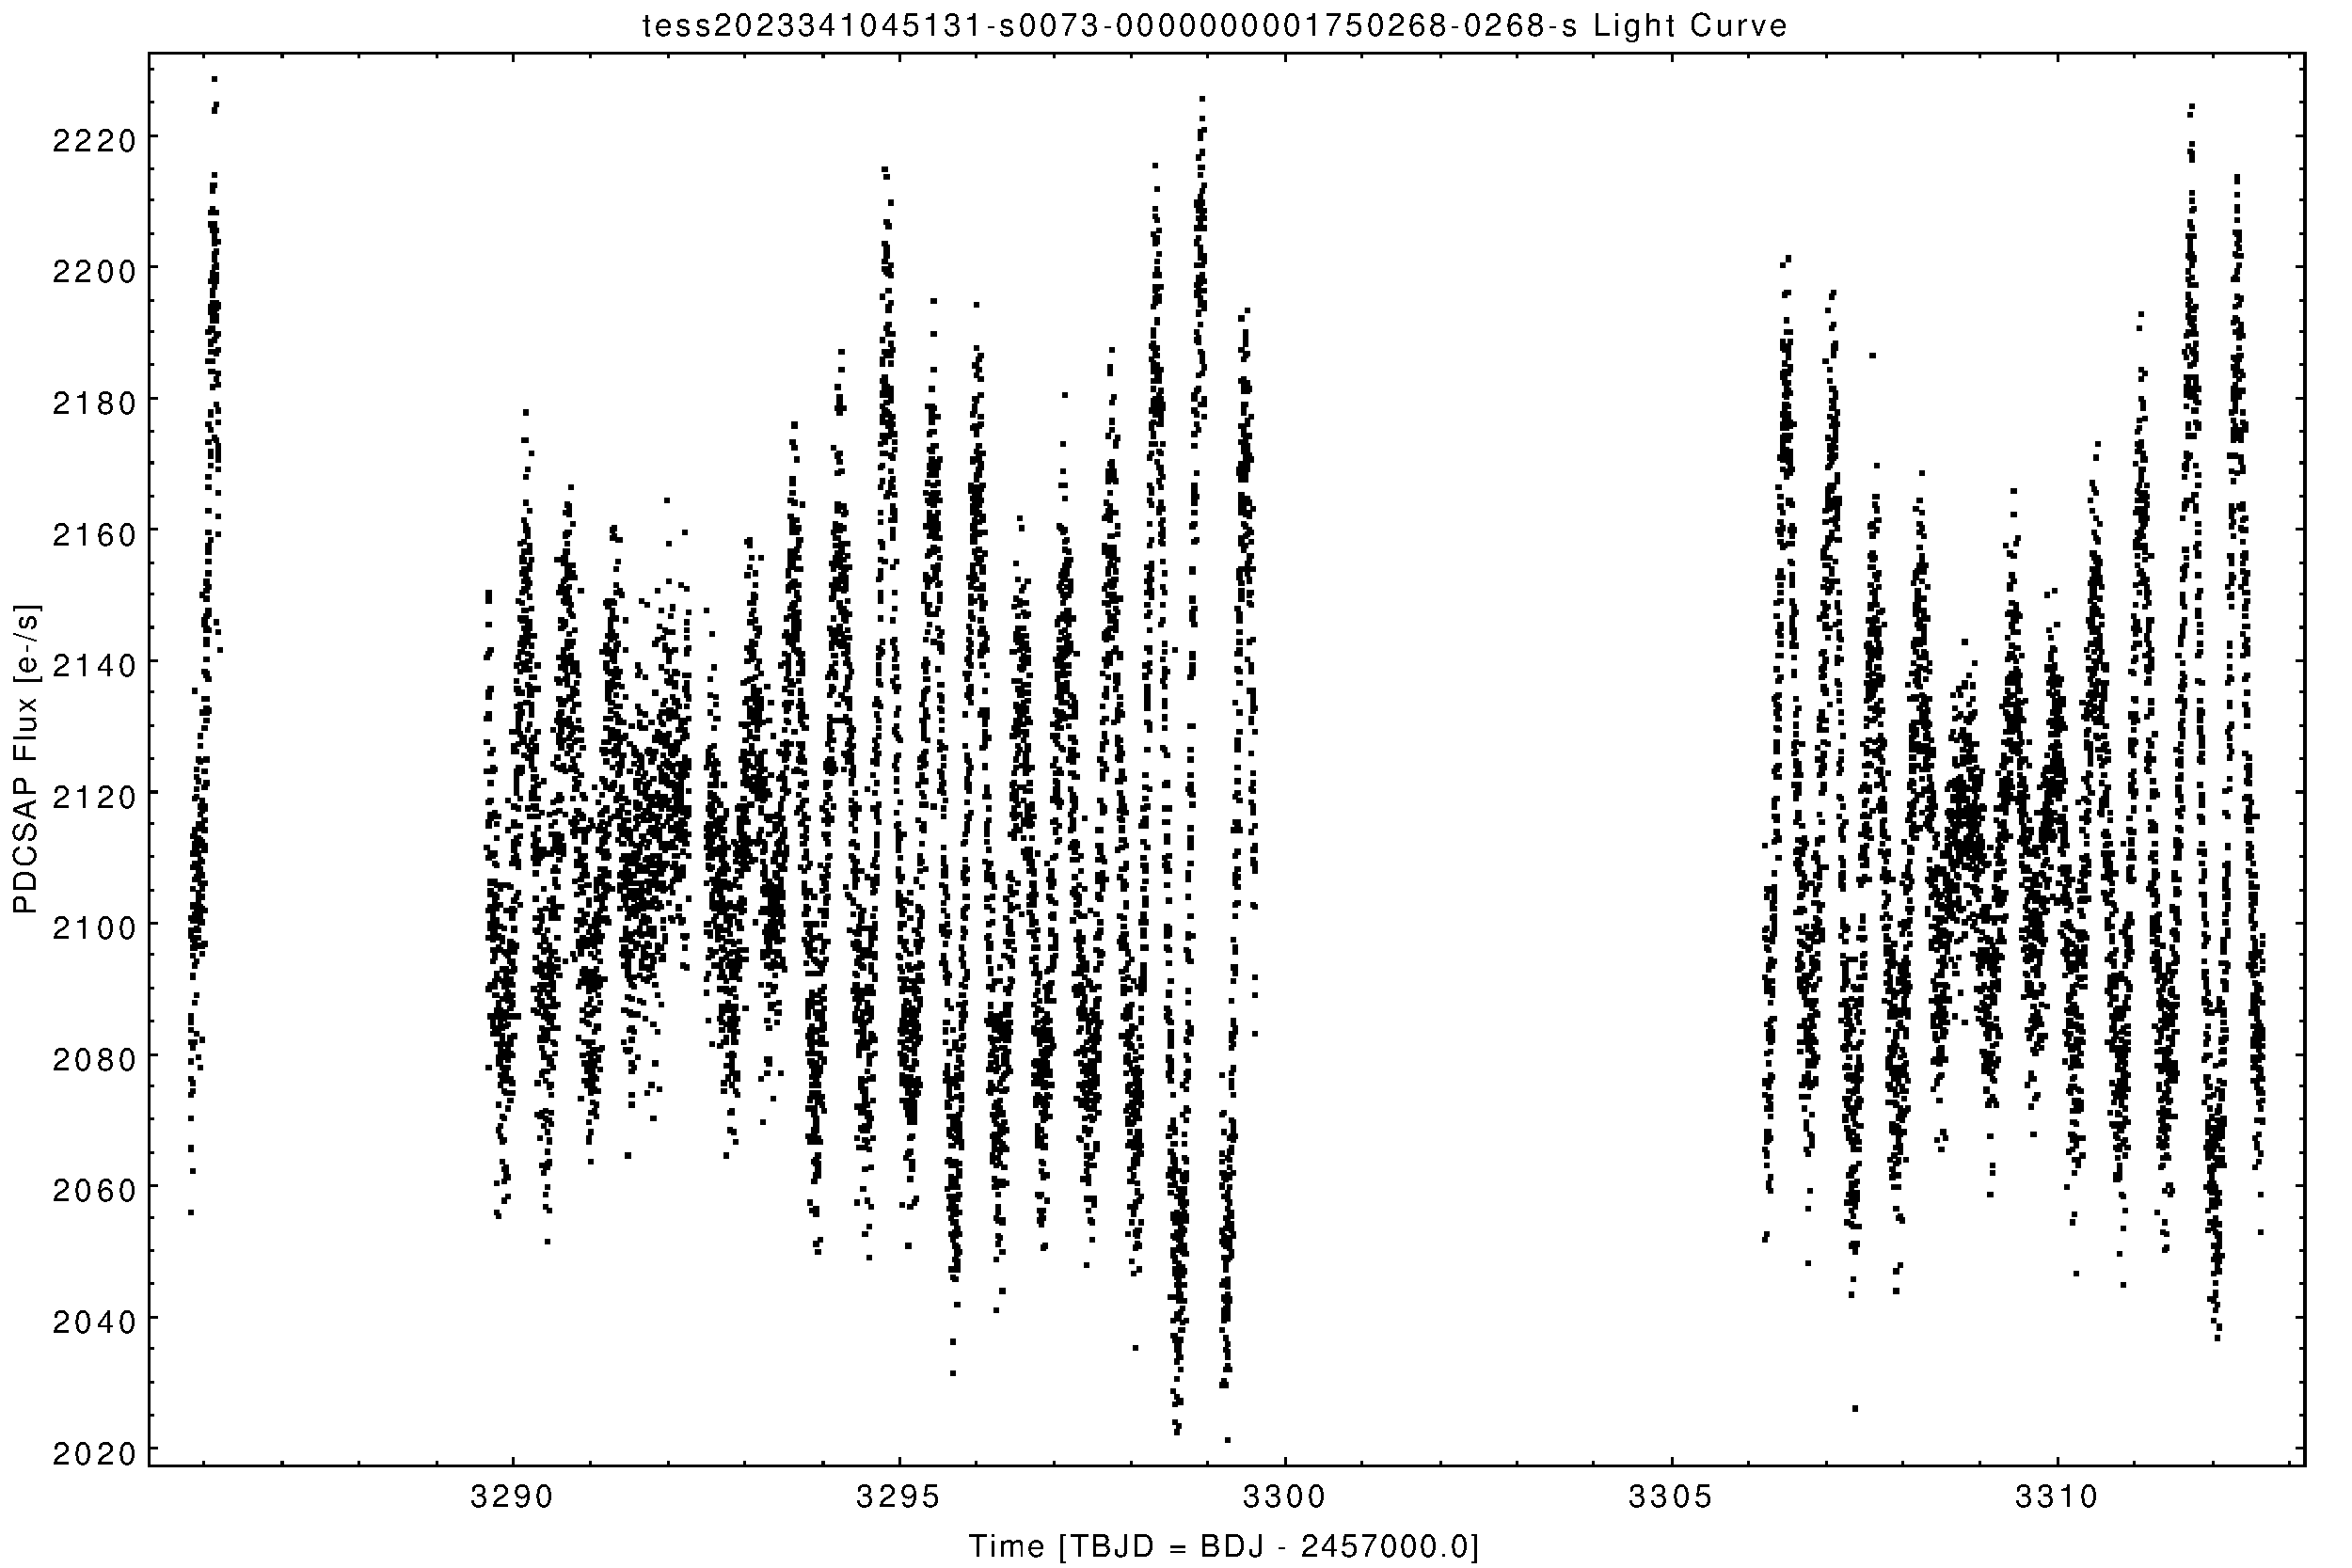
\includegraphics[width = 1\textwidth]{
      lightcurves/tess2023341045131-s0073-0000000001750268-0268-s.pdf}
    \caption{tess2023341045131-s0073-0000000001750268-0268-s light curve}
\end{figure}
\begin{figure}[htbp]
    \centering
    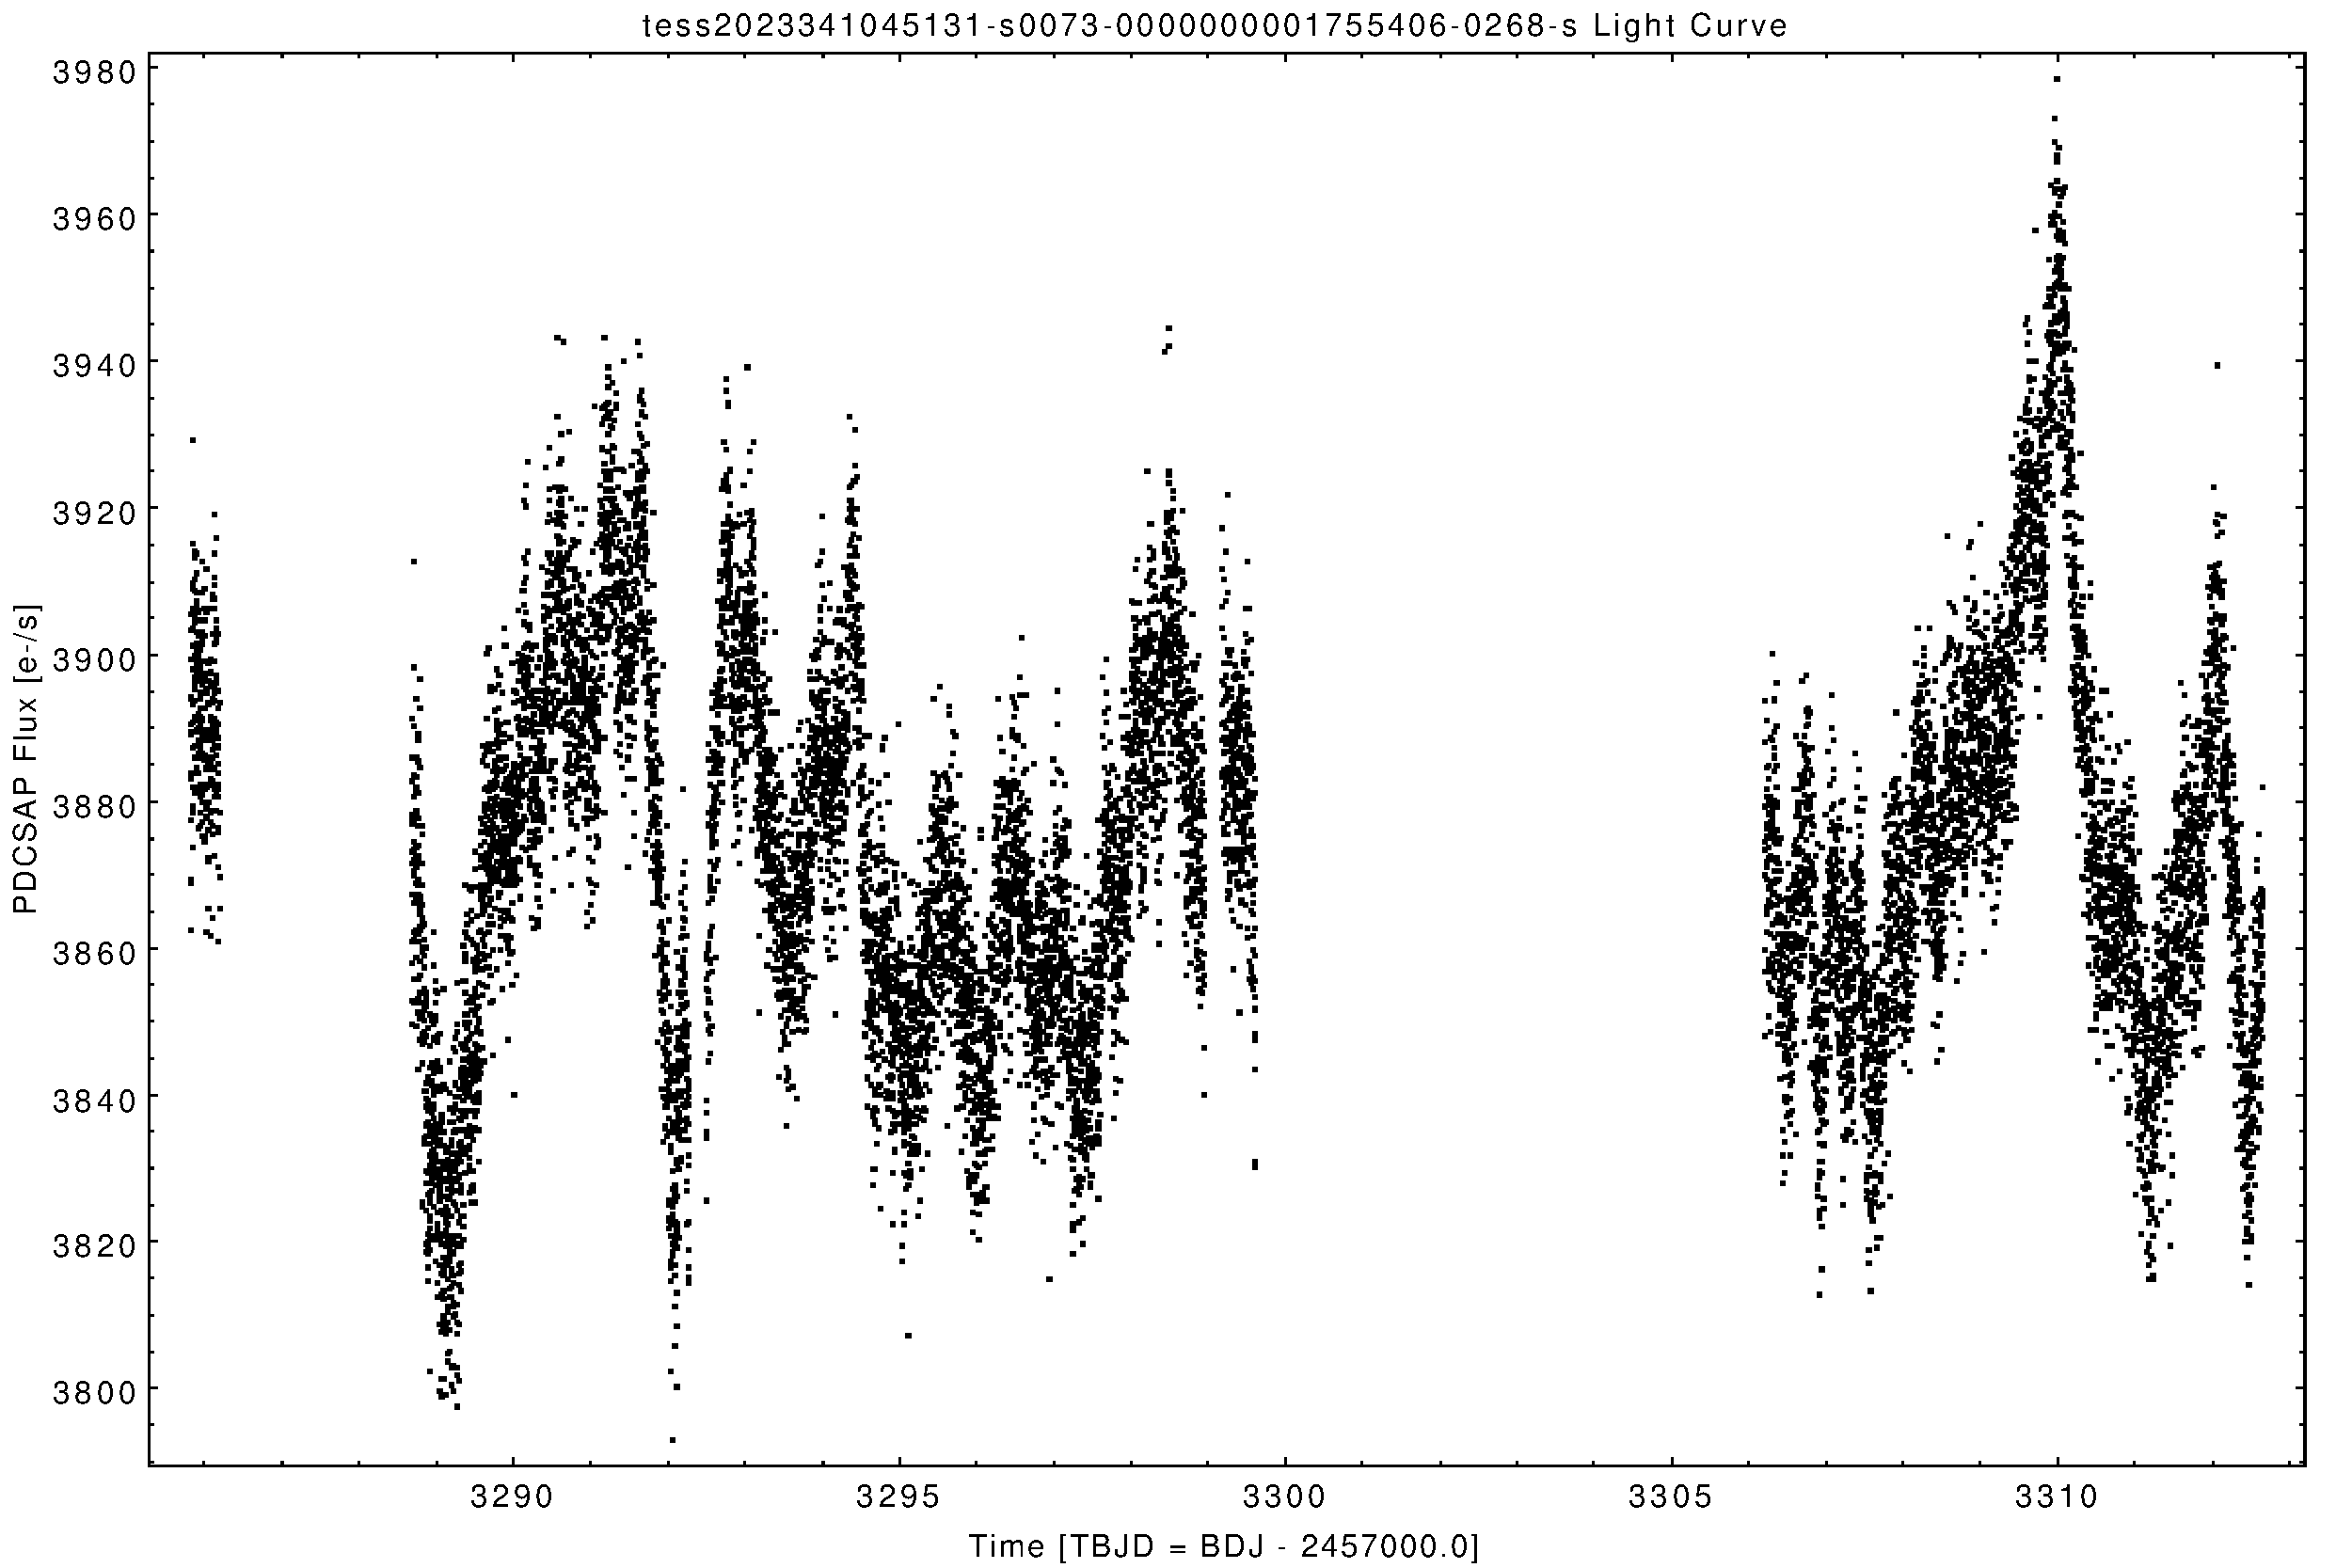
\includegraphics[width = 1\textwidth]{
      lightcurves/tess2023341045131-s0073-0000000001755406-0268-s.pdf}
    \caption{tess2023341045131-s0073-0000000001755406-0268-s light curve}
\end{figure}
\begin{figure}[htbp]
    \centering
    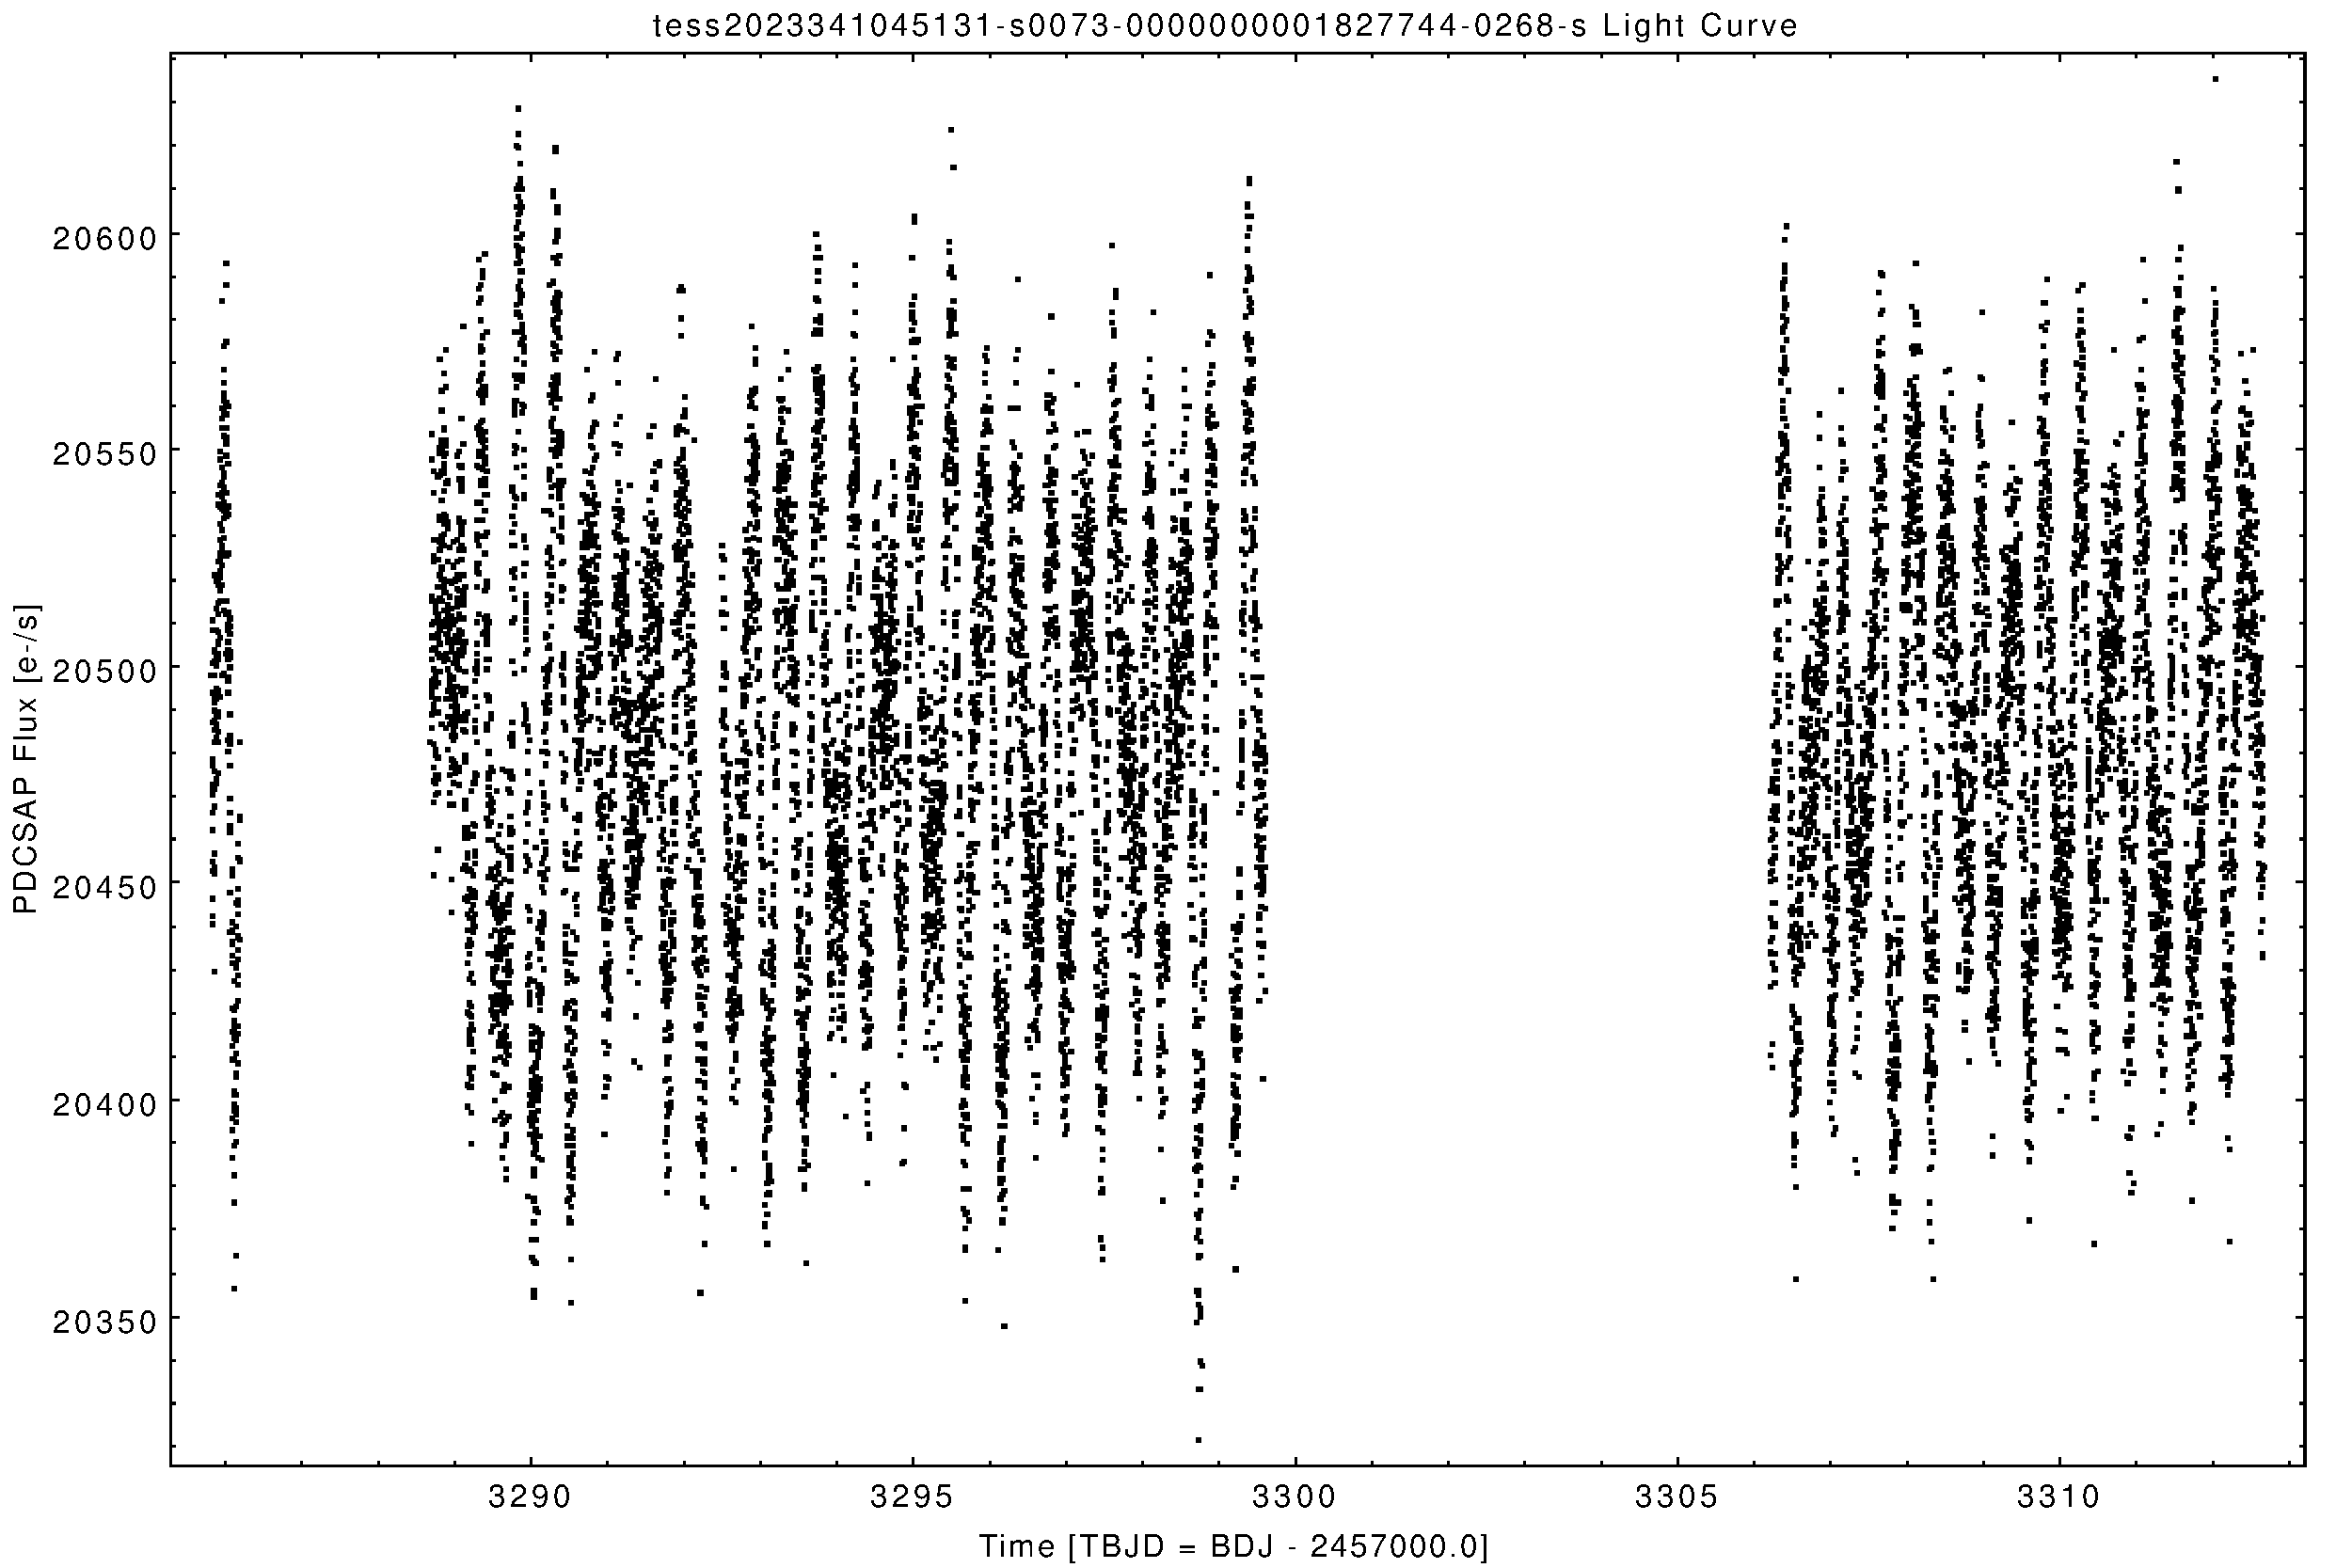
\includegraphics[width = 1\textwidth]{
      lightcurves/tess2023341045131-s0073-0000000001827744-0268-s.pdf}
    \caption{tess2023341045131-s0073-0000000001827744-0268-s light curve}
\end{figure}
\begin{figure}[htbp]
    \centering
    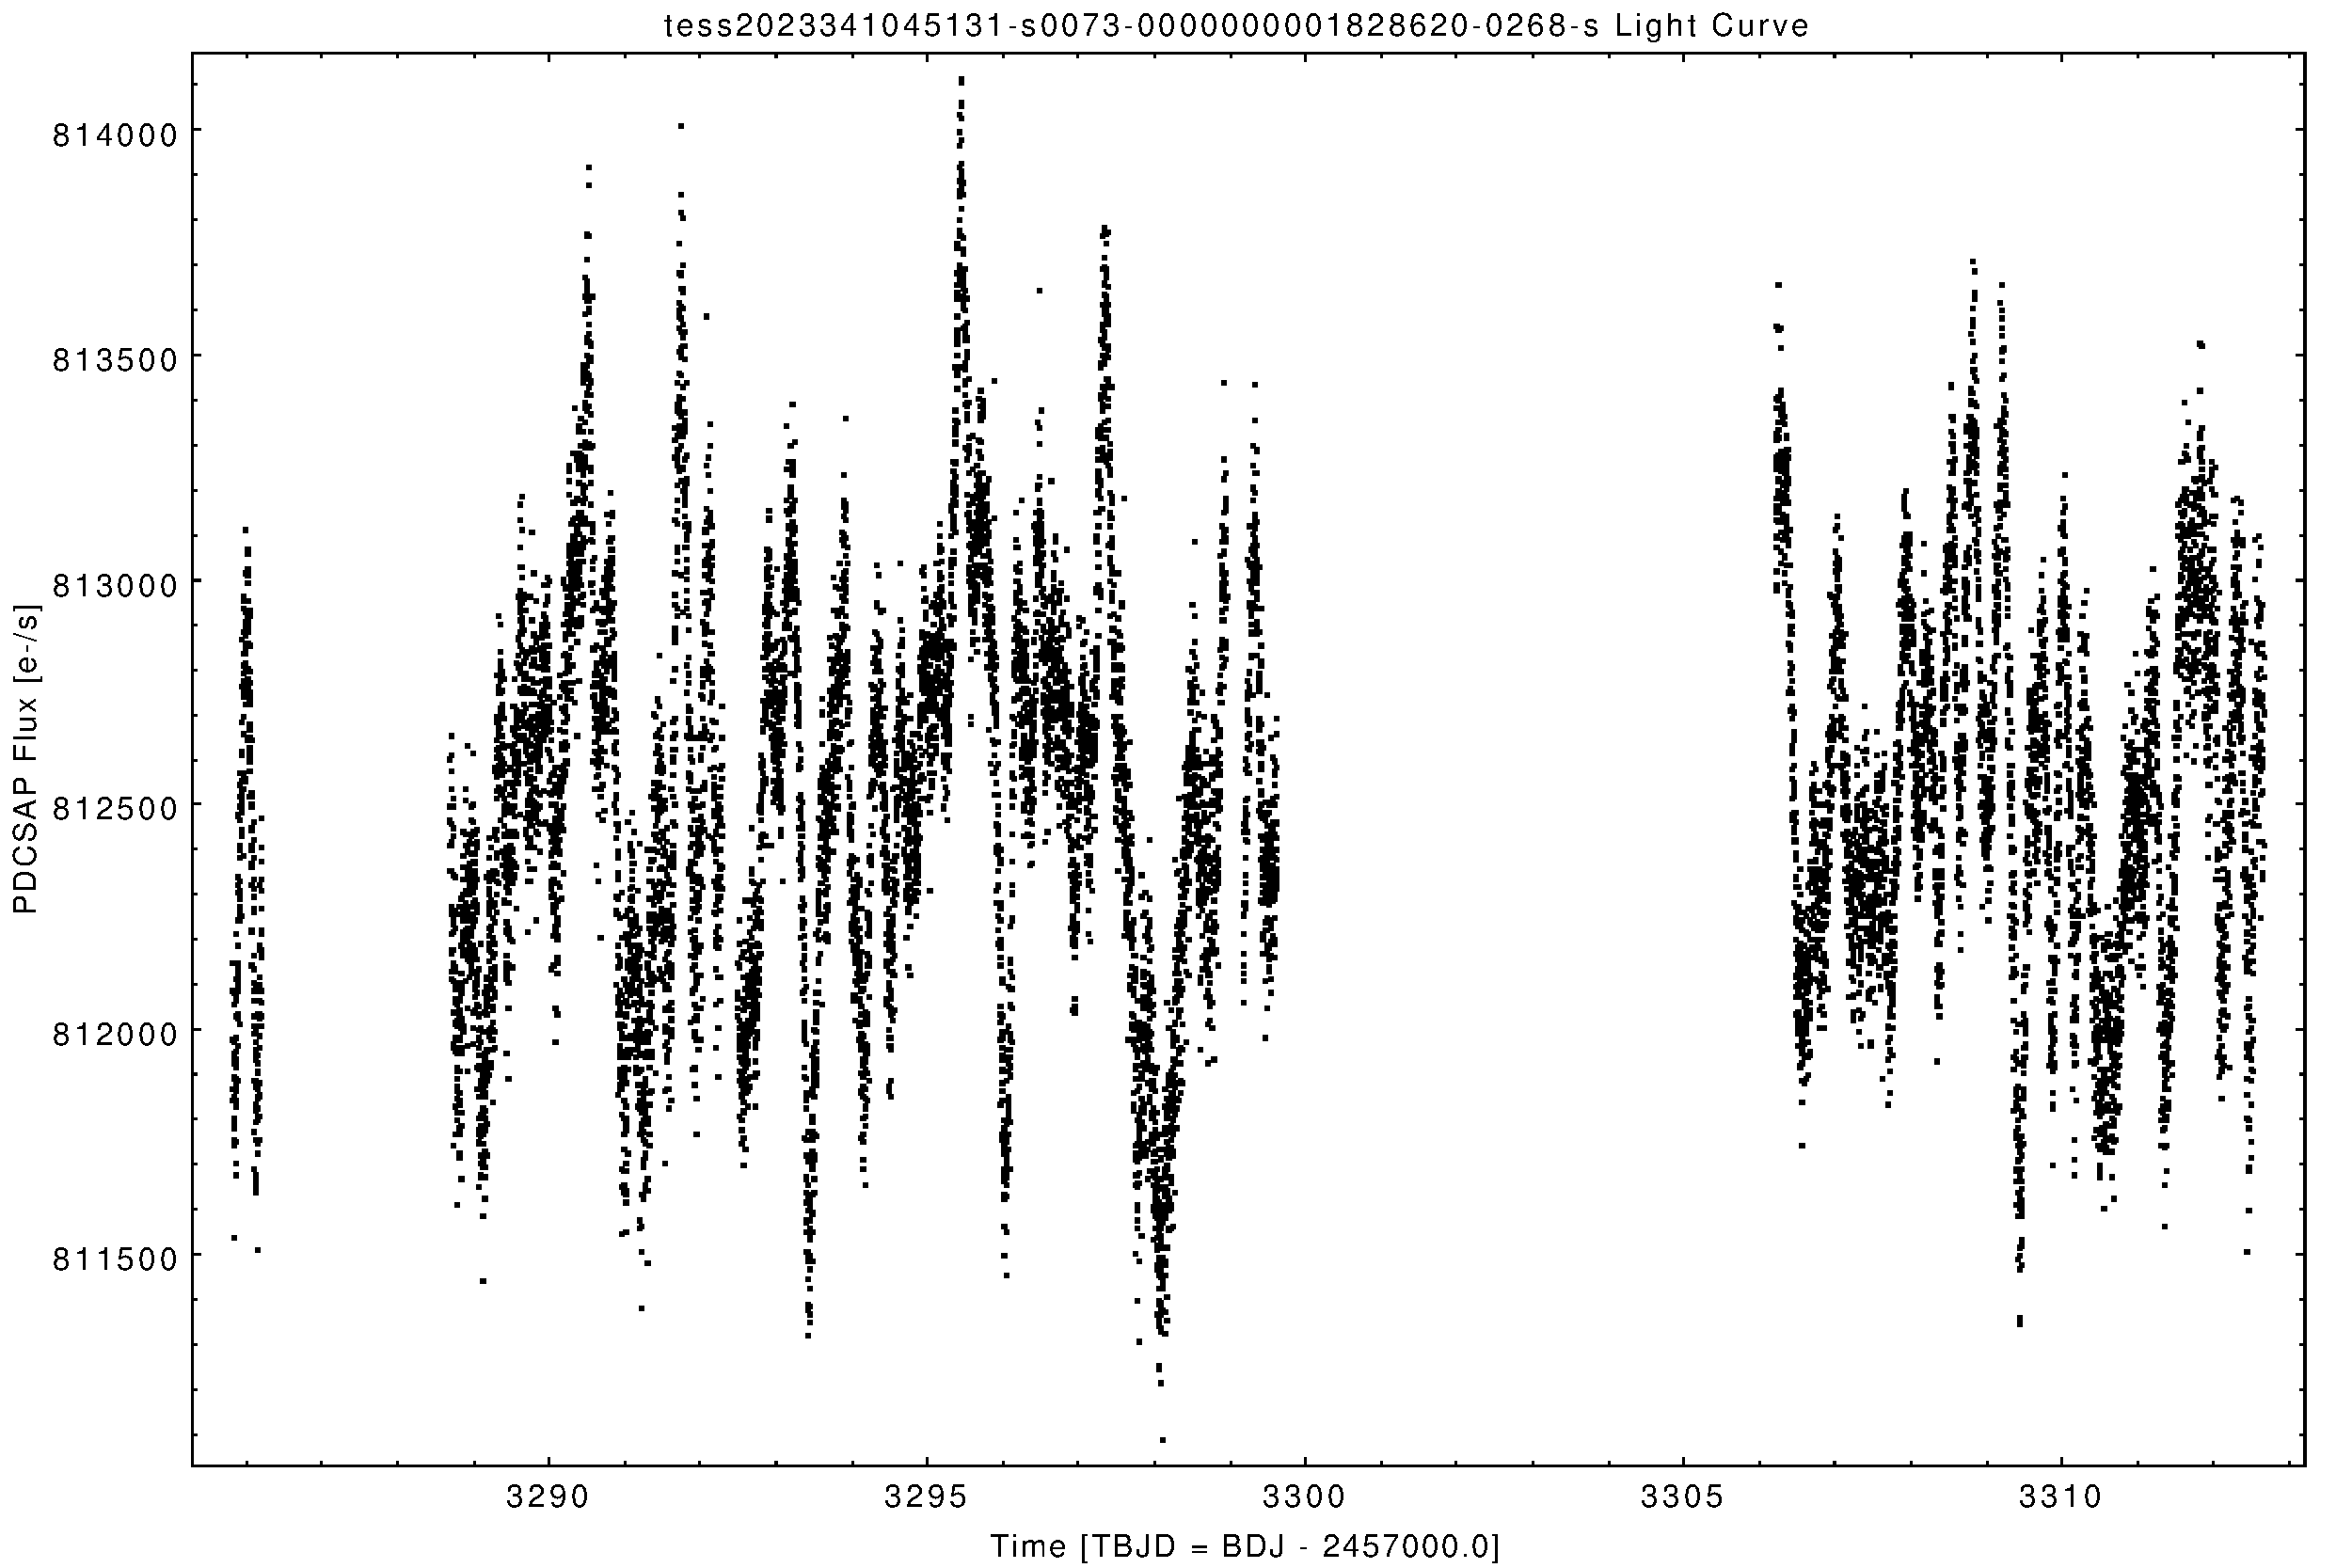
\includegraphics[width = 1\textwidth]{
      lightcurves/tess2023341045131-s0073-0000000001828620-0268-s.pdf}
    \caption{tess2023341045131-s0073-0000000001828620-0268-s light curve}
\end{figure}
\begin{figure}[htbp]
    \centering
    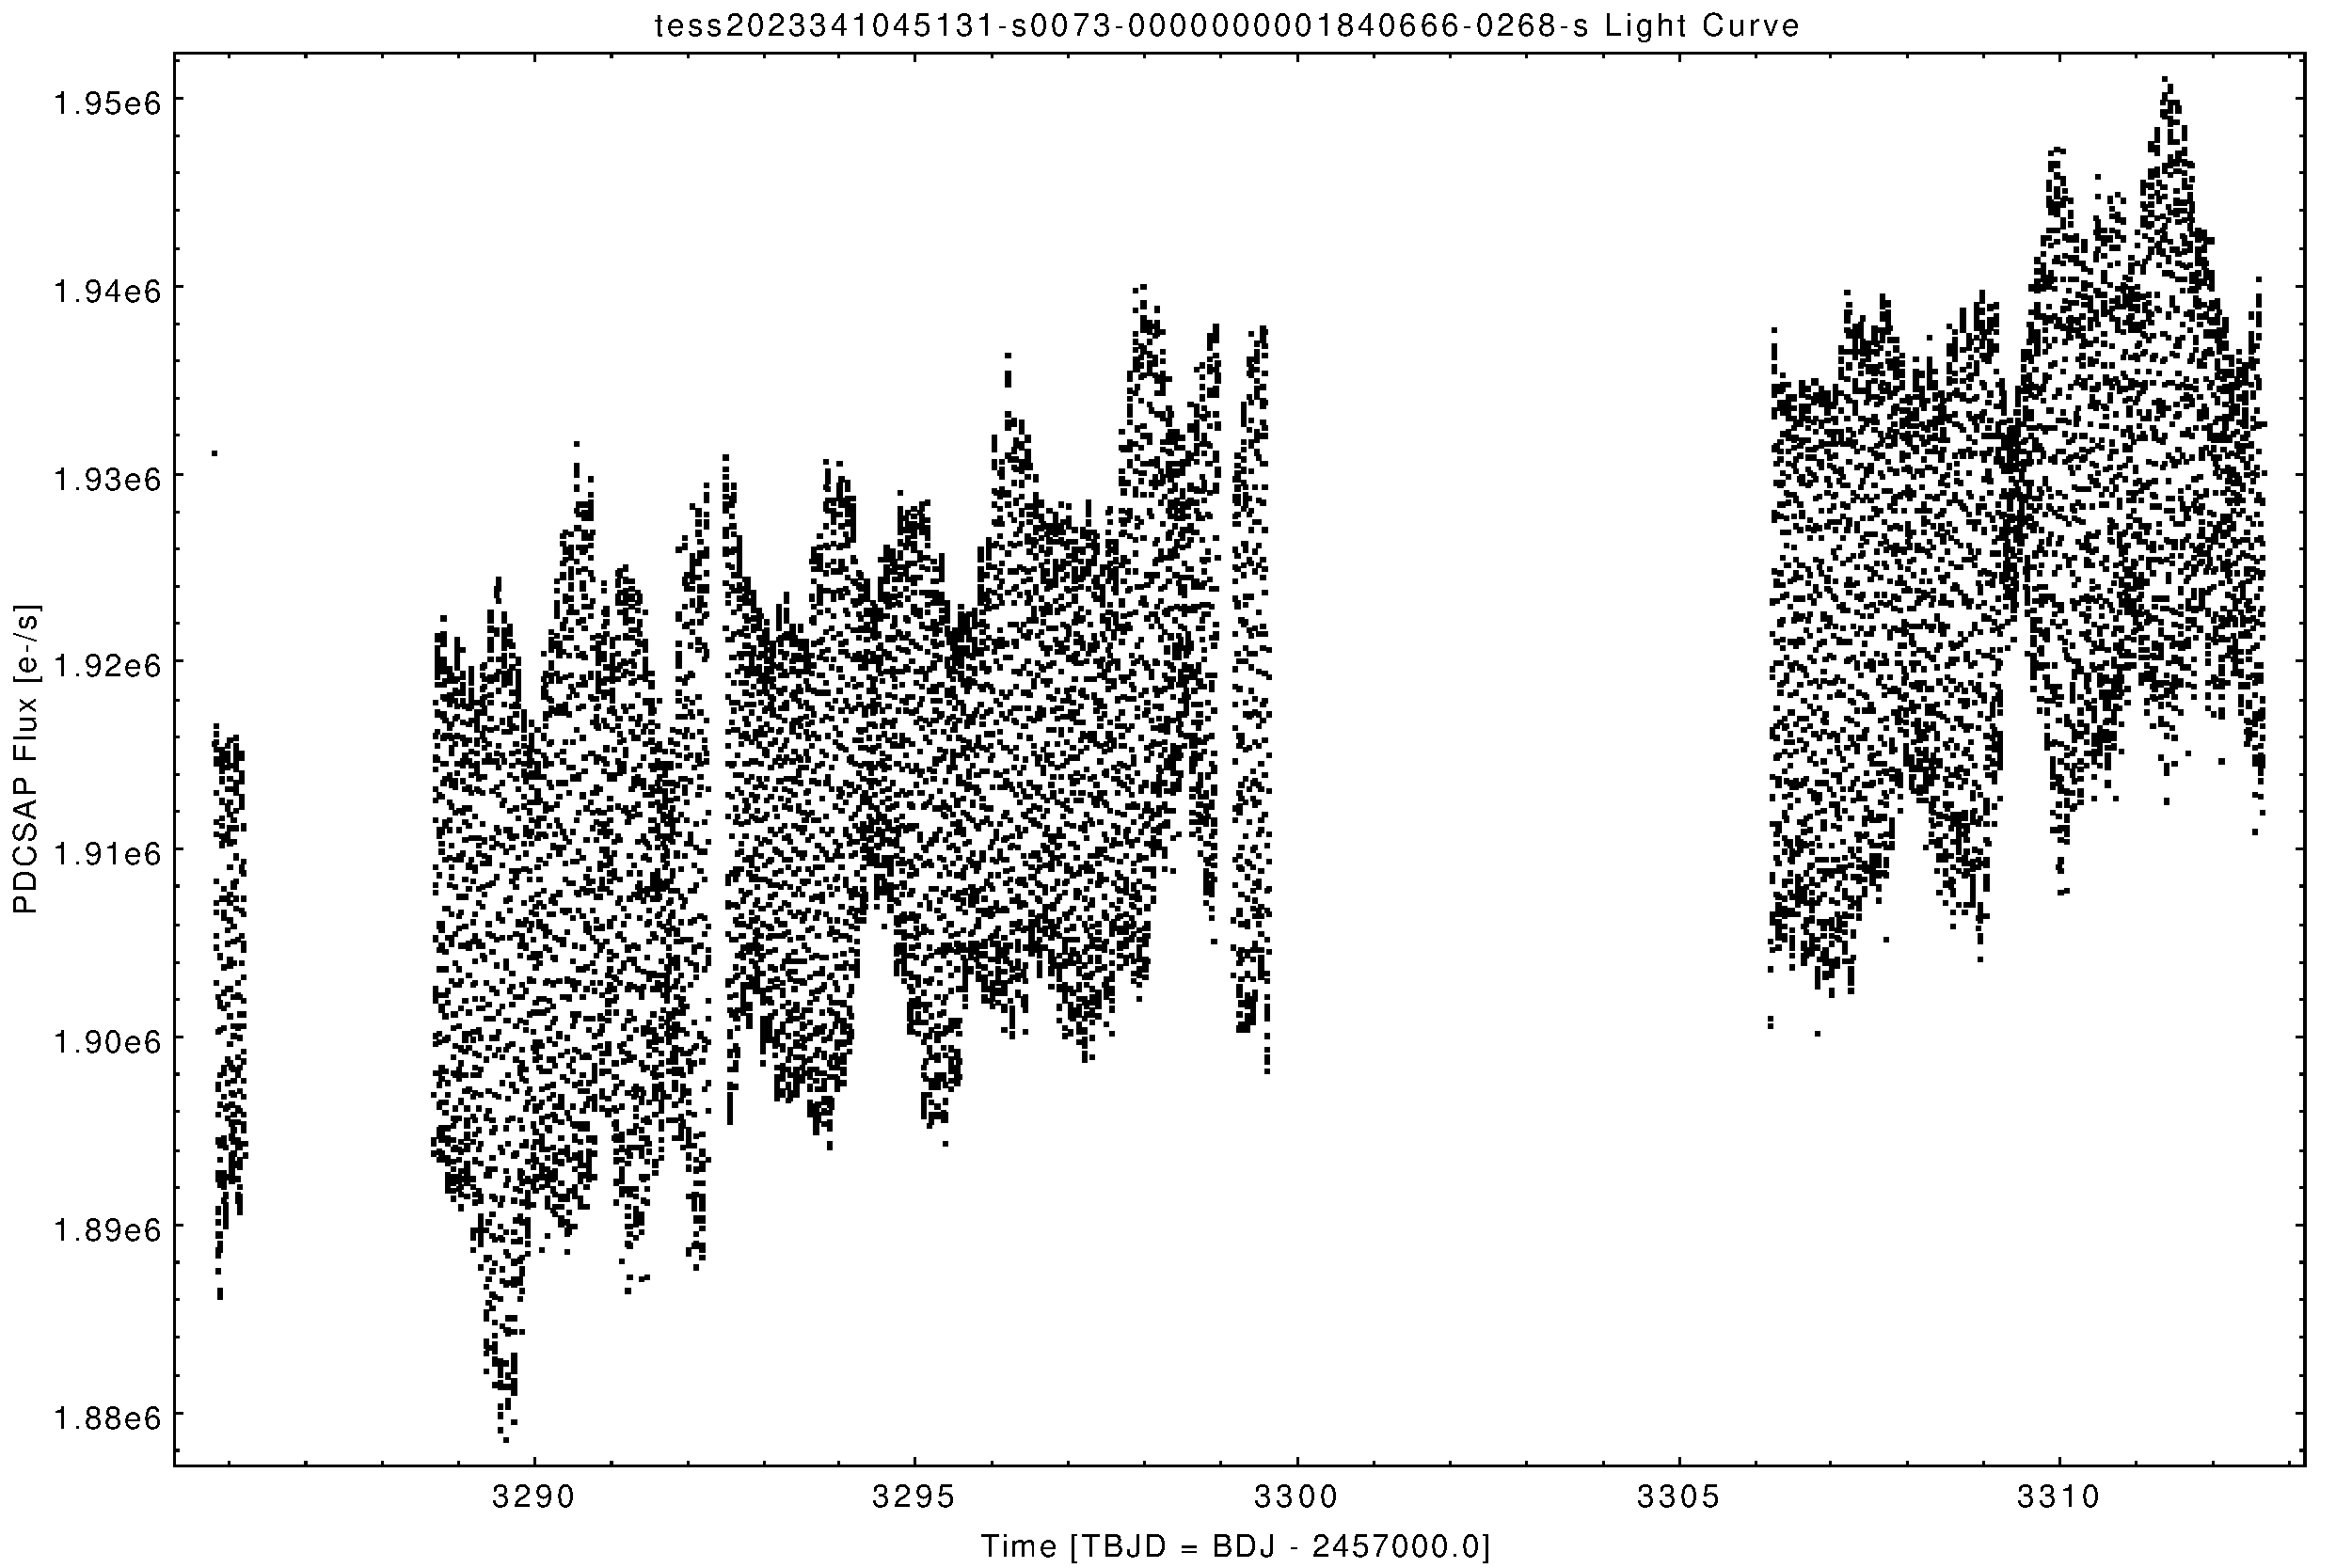
\includegraphics[width = 1\textwidth]{
      lightcurves/tess2023341045131-s0073-0000000001840666-0268-s.pdf}
    \caption{tess2023341045131-s0073-0000000001840666-0268-s light curve}
\end{figure}
\begin{figure}[htbp]
    \centering
    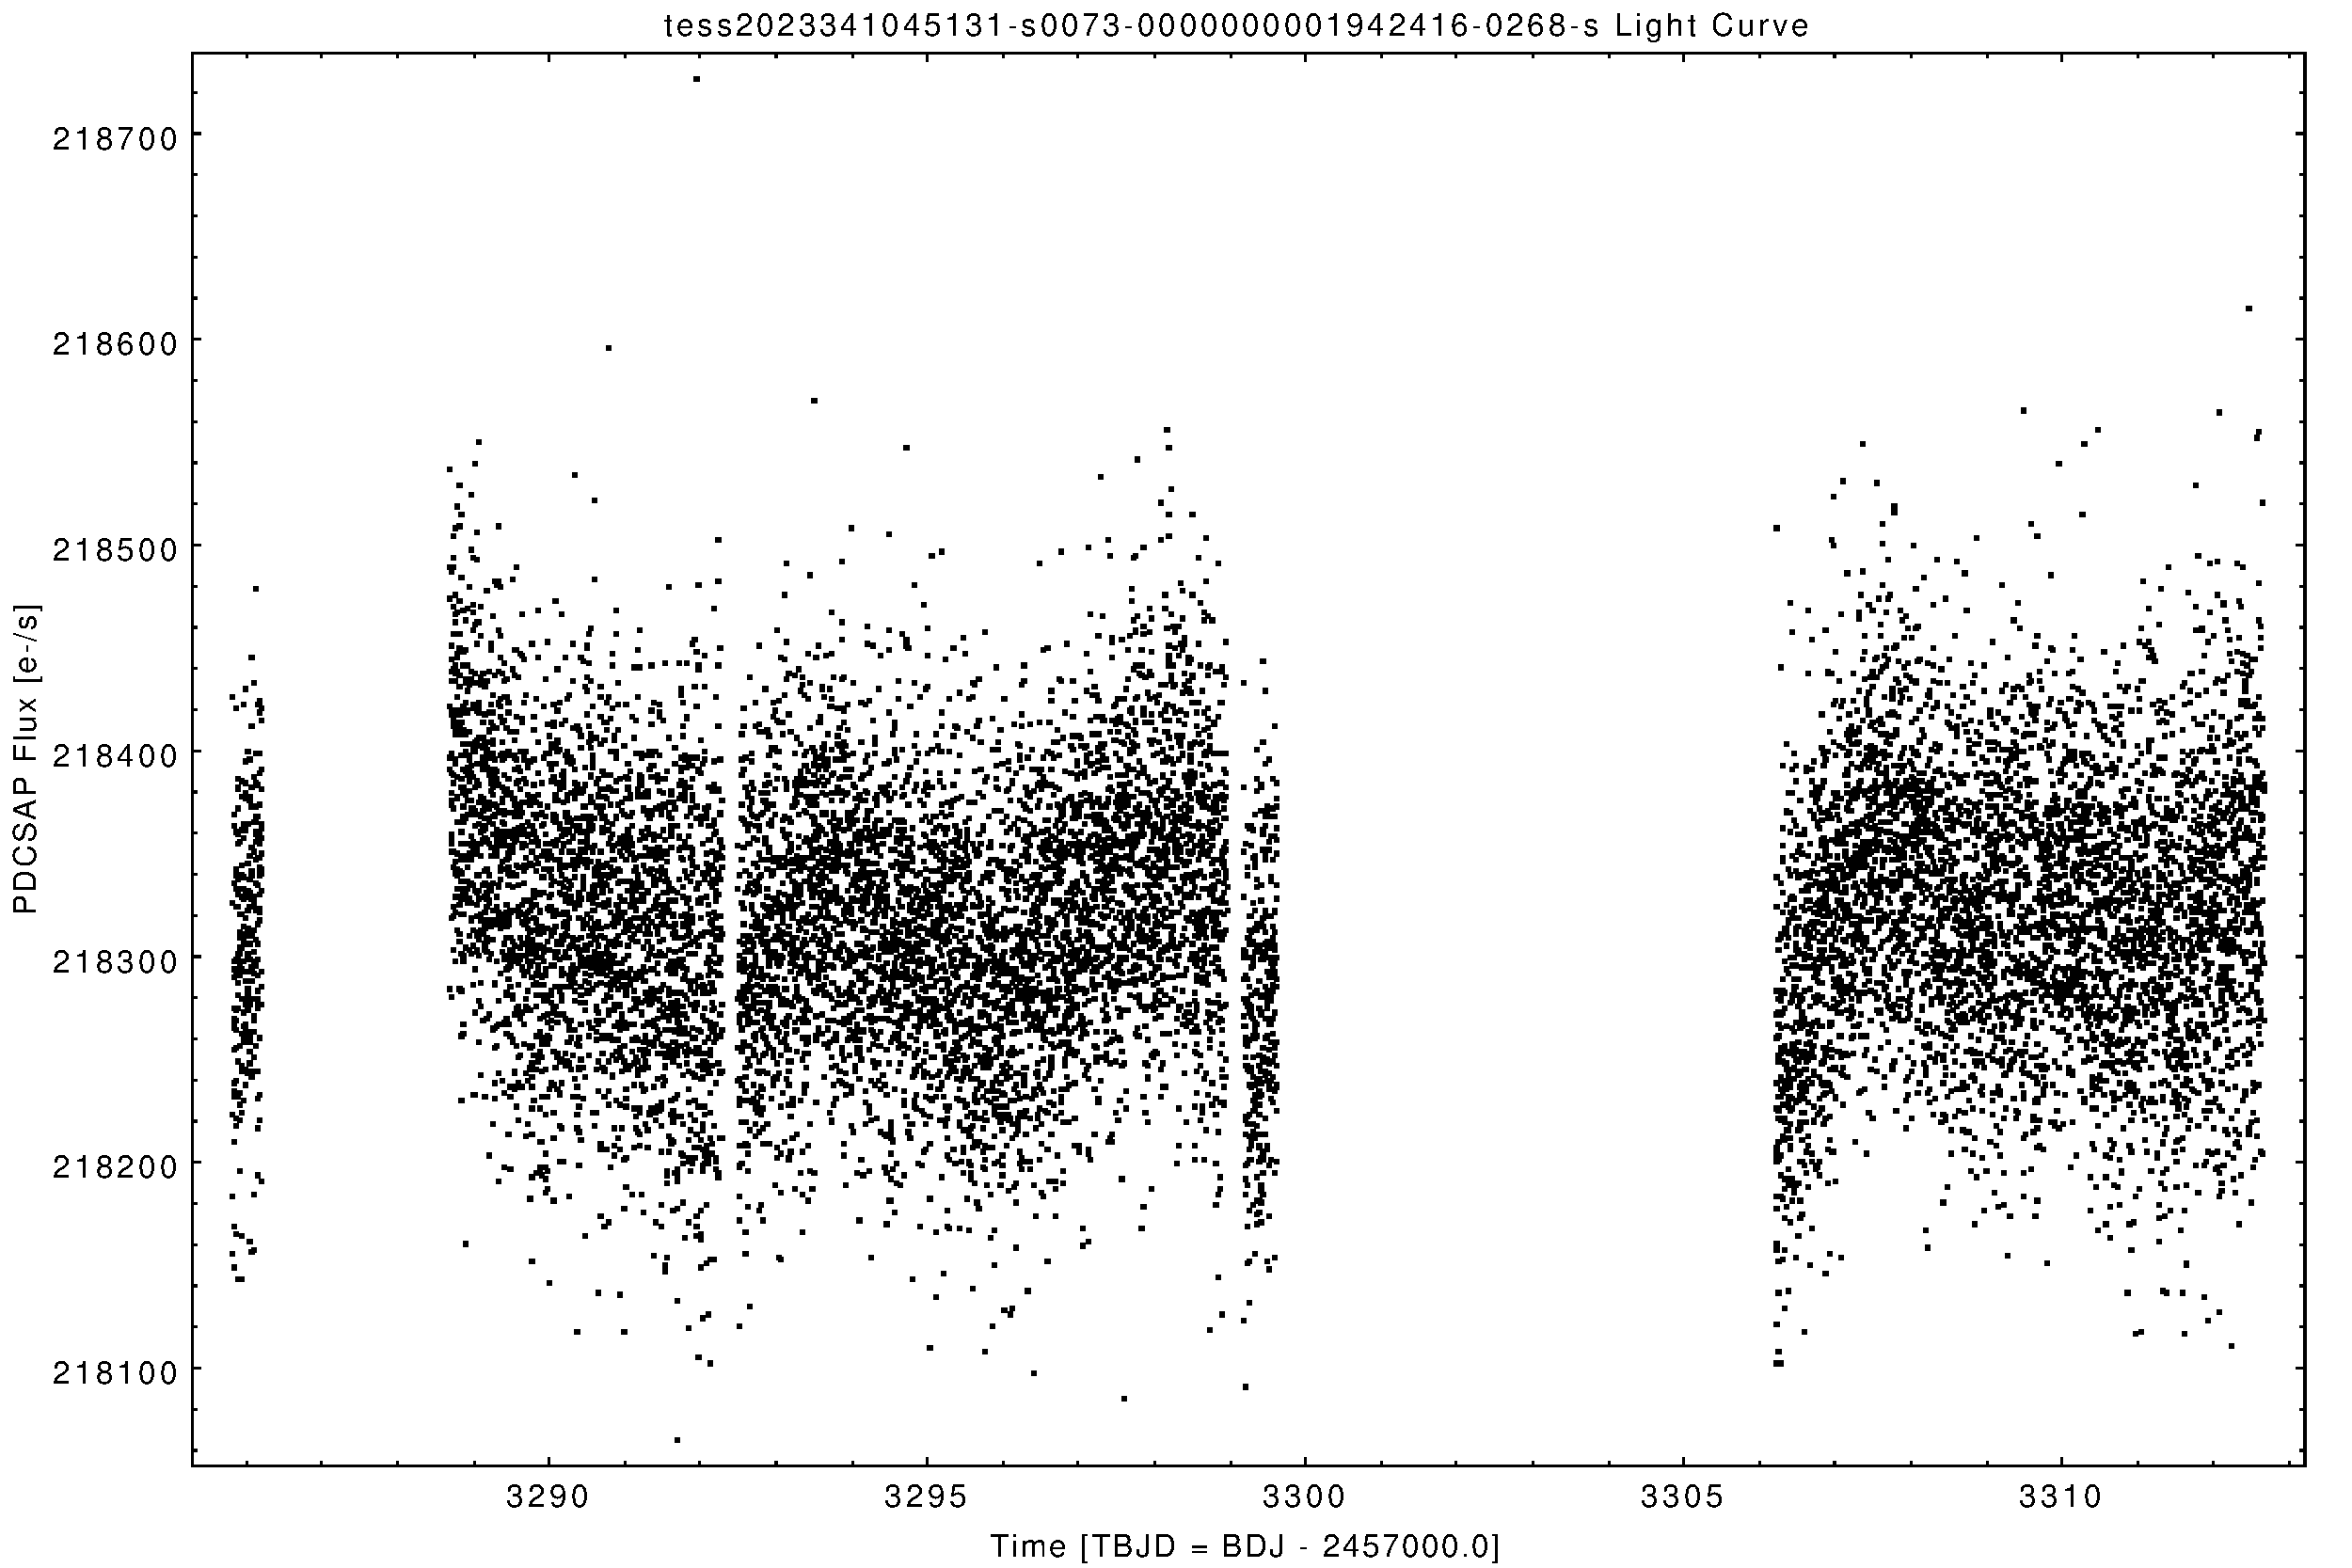
\includegraphics[width = 1\textwidth]{
      lightcurves/tess2023341045131-s0073-0000000001942416-0268-s.pdf}
    \caption{tess2023341045131-s0073-0000000001942416-0268-s light curve}
\end{figure}
\begin{figure}[htbp]
    \centering
    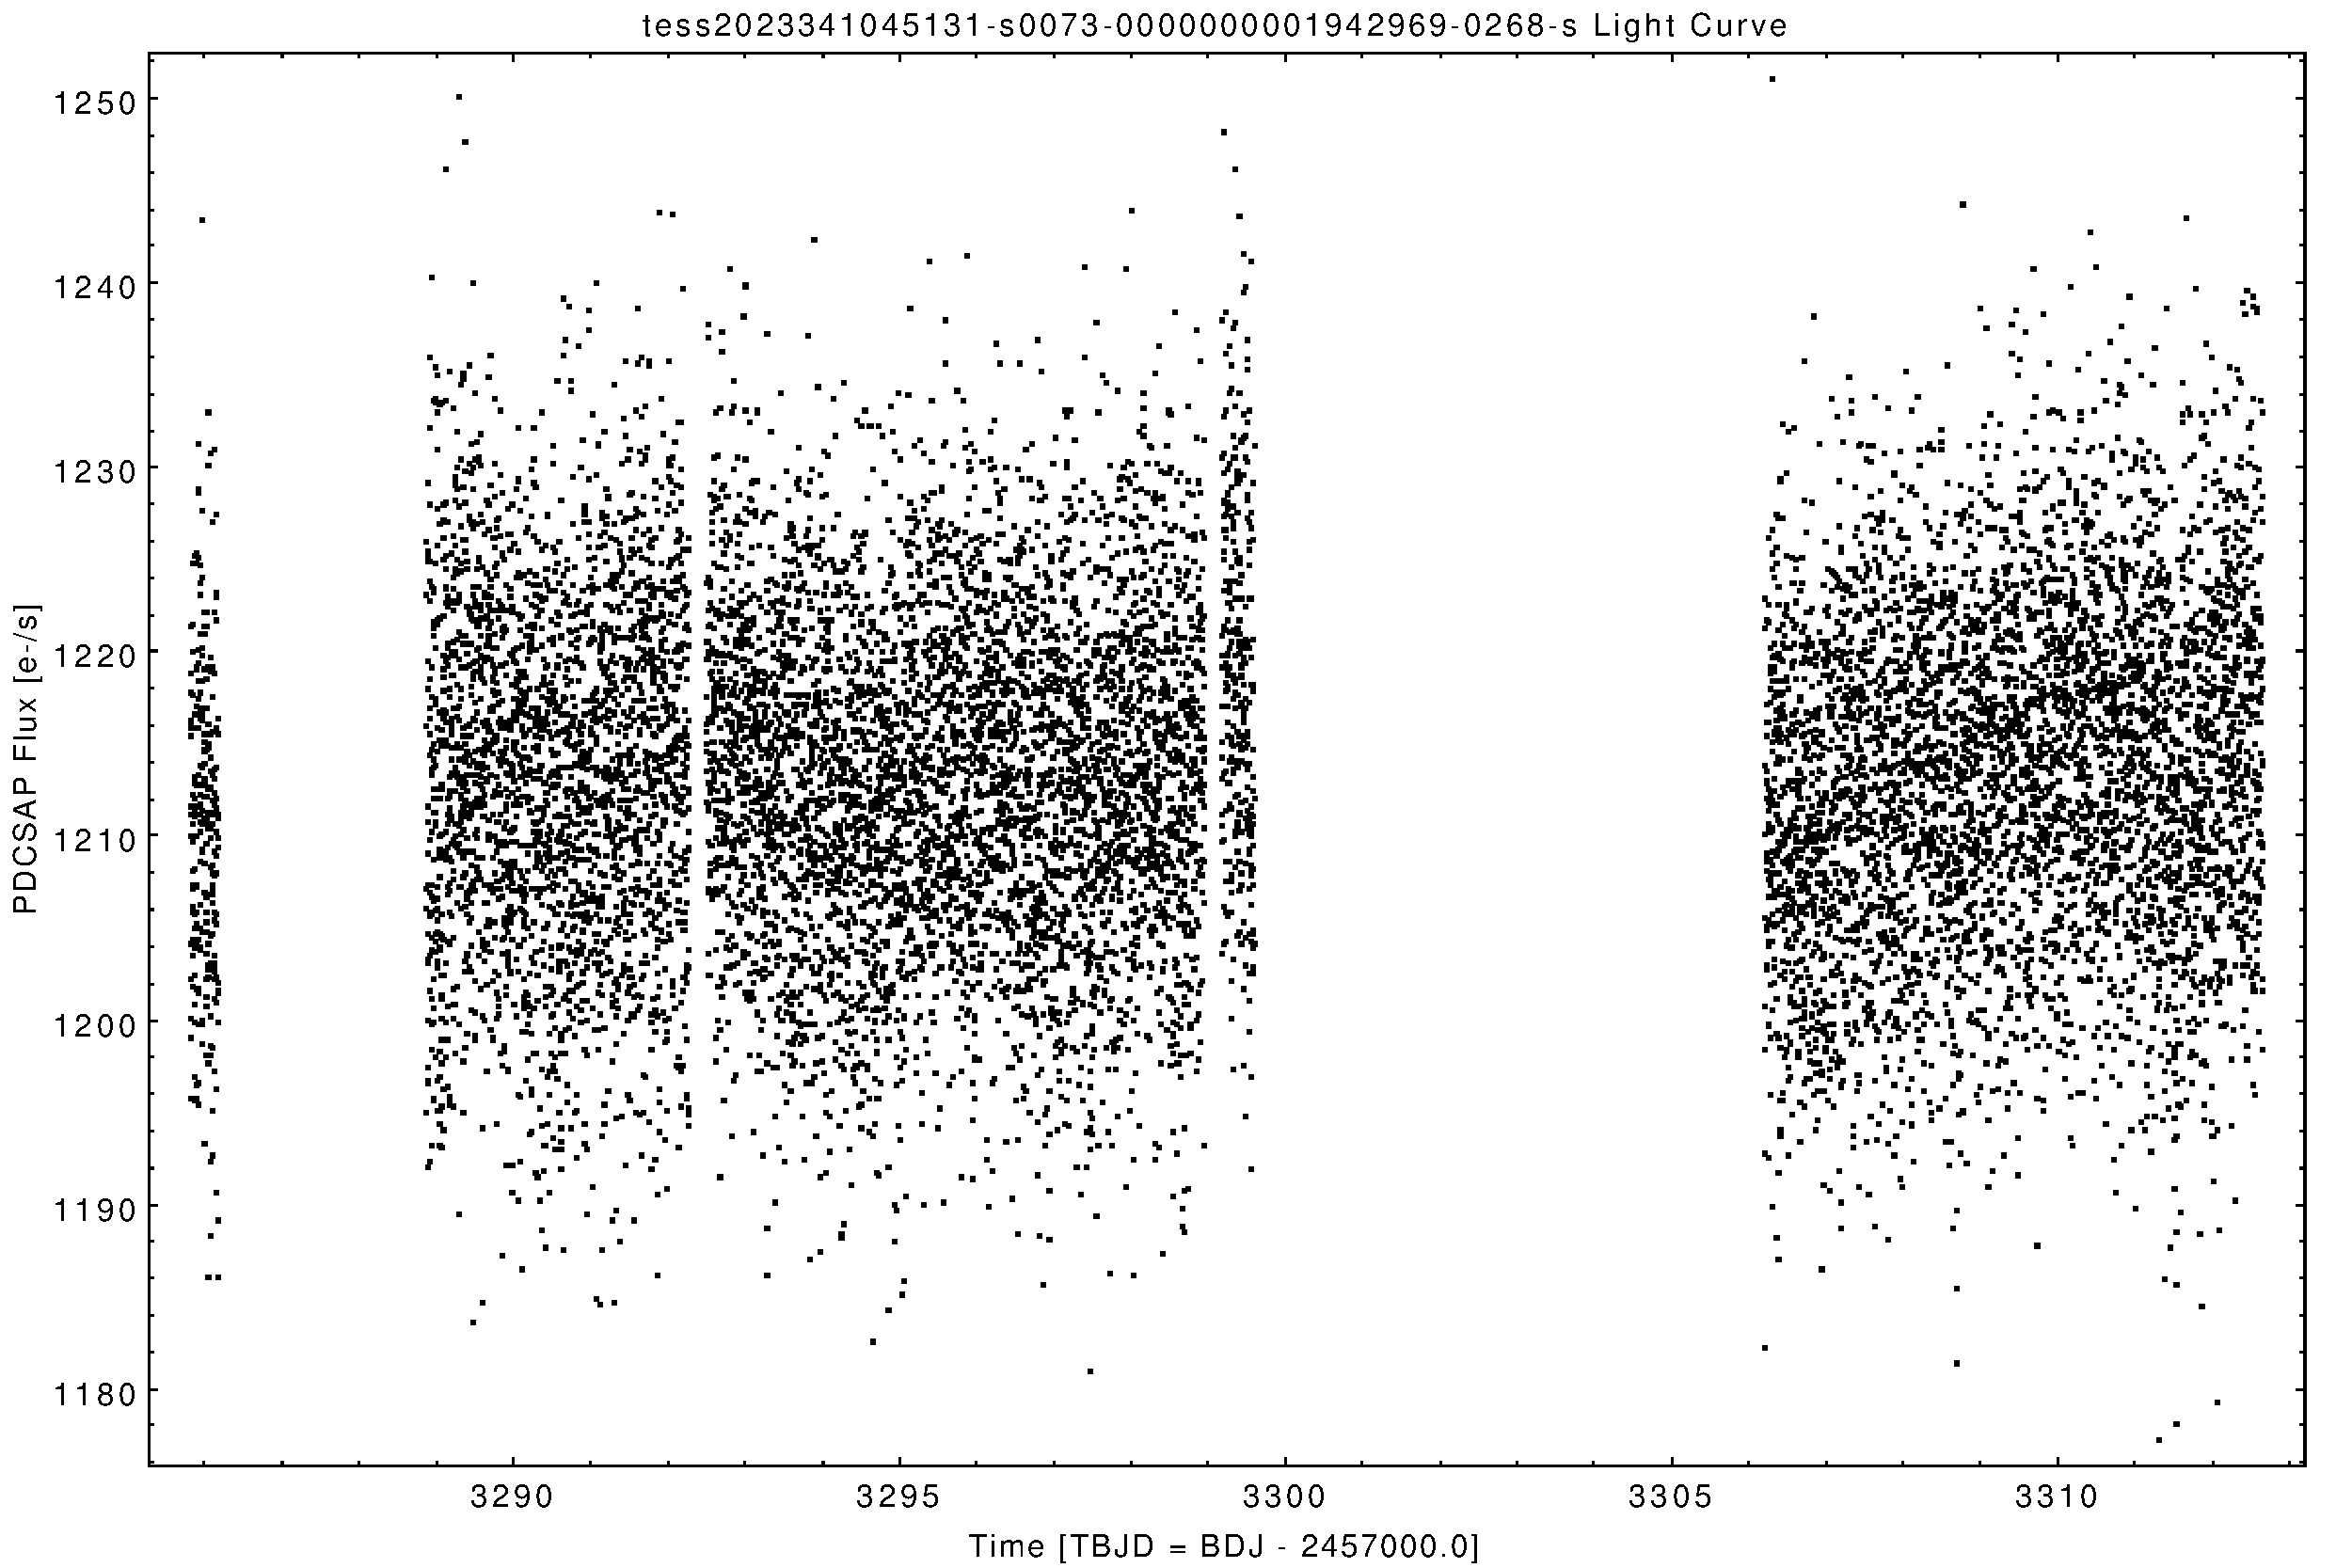
\includegraphics[width = 1\textwidth]{
      lightcurves/tess2023341045131-s0073-0000000001942969-0268-s.pdf}
    \caption{tess2023341045131-s0073-0000000001942969-0268-s light curve}
\end{figure}
\begin{figure}[htbp]
    \centering
    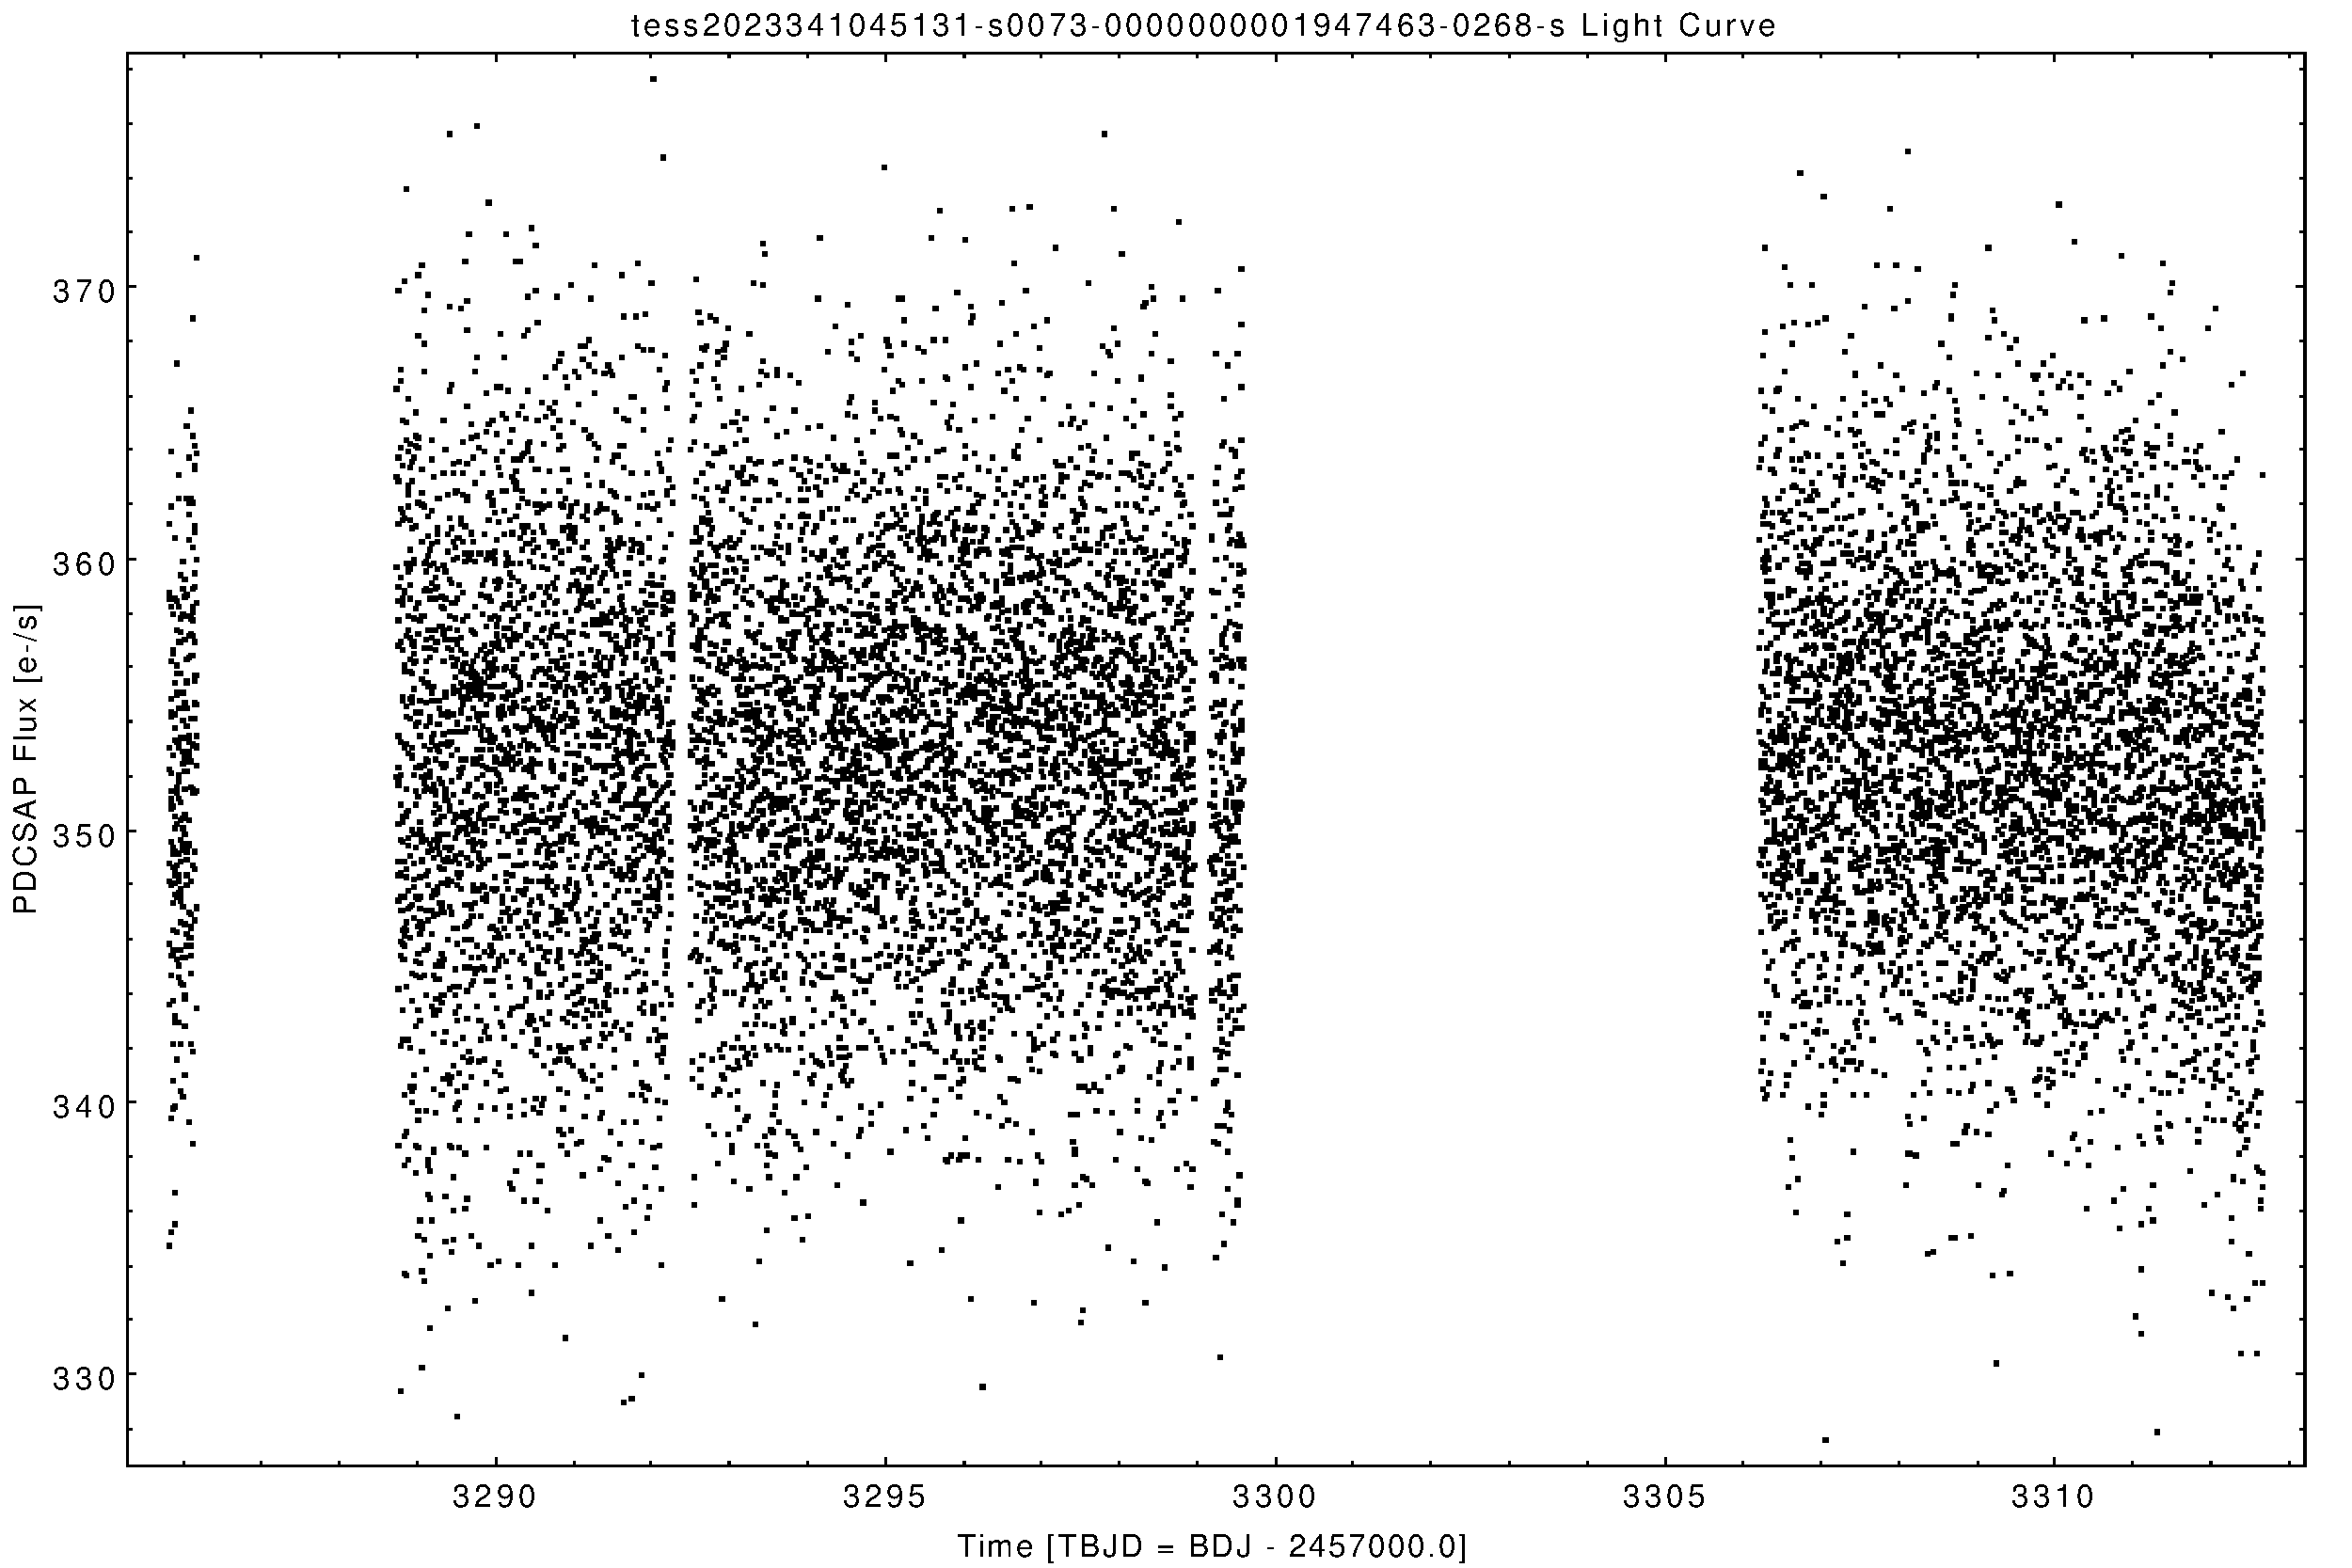
\includegraphics[width = 1\textwidth]{
      lightcurves/tess2023341045131-s0073-0000000001947463-0268-s.pdf}
    \caption{tess2023341045131-s0073-0000000001947463-0268-s light curve}
\end{figure}
\begin{figure}[htbp]
    \centering
    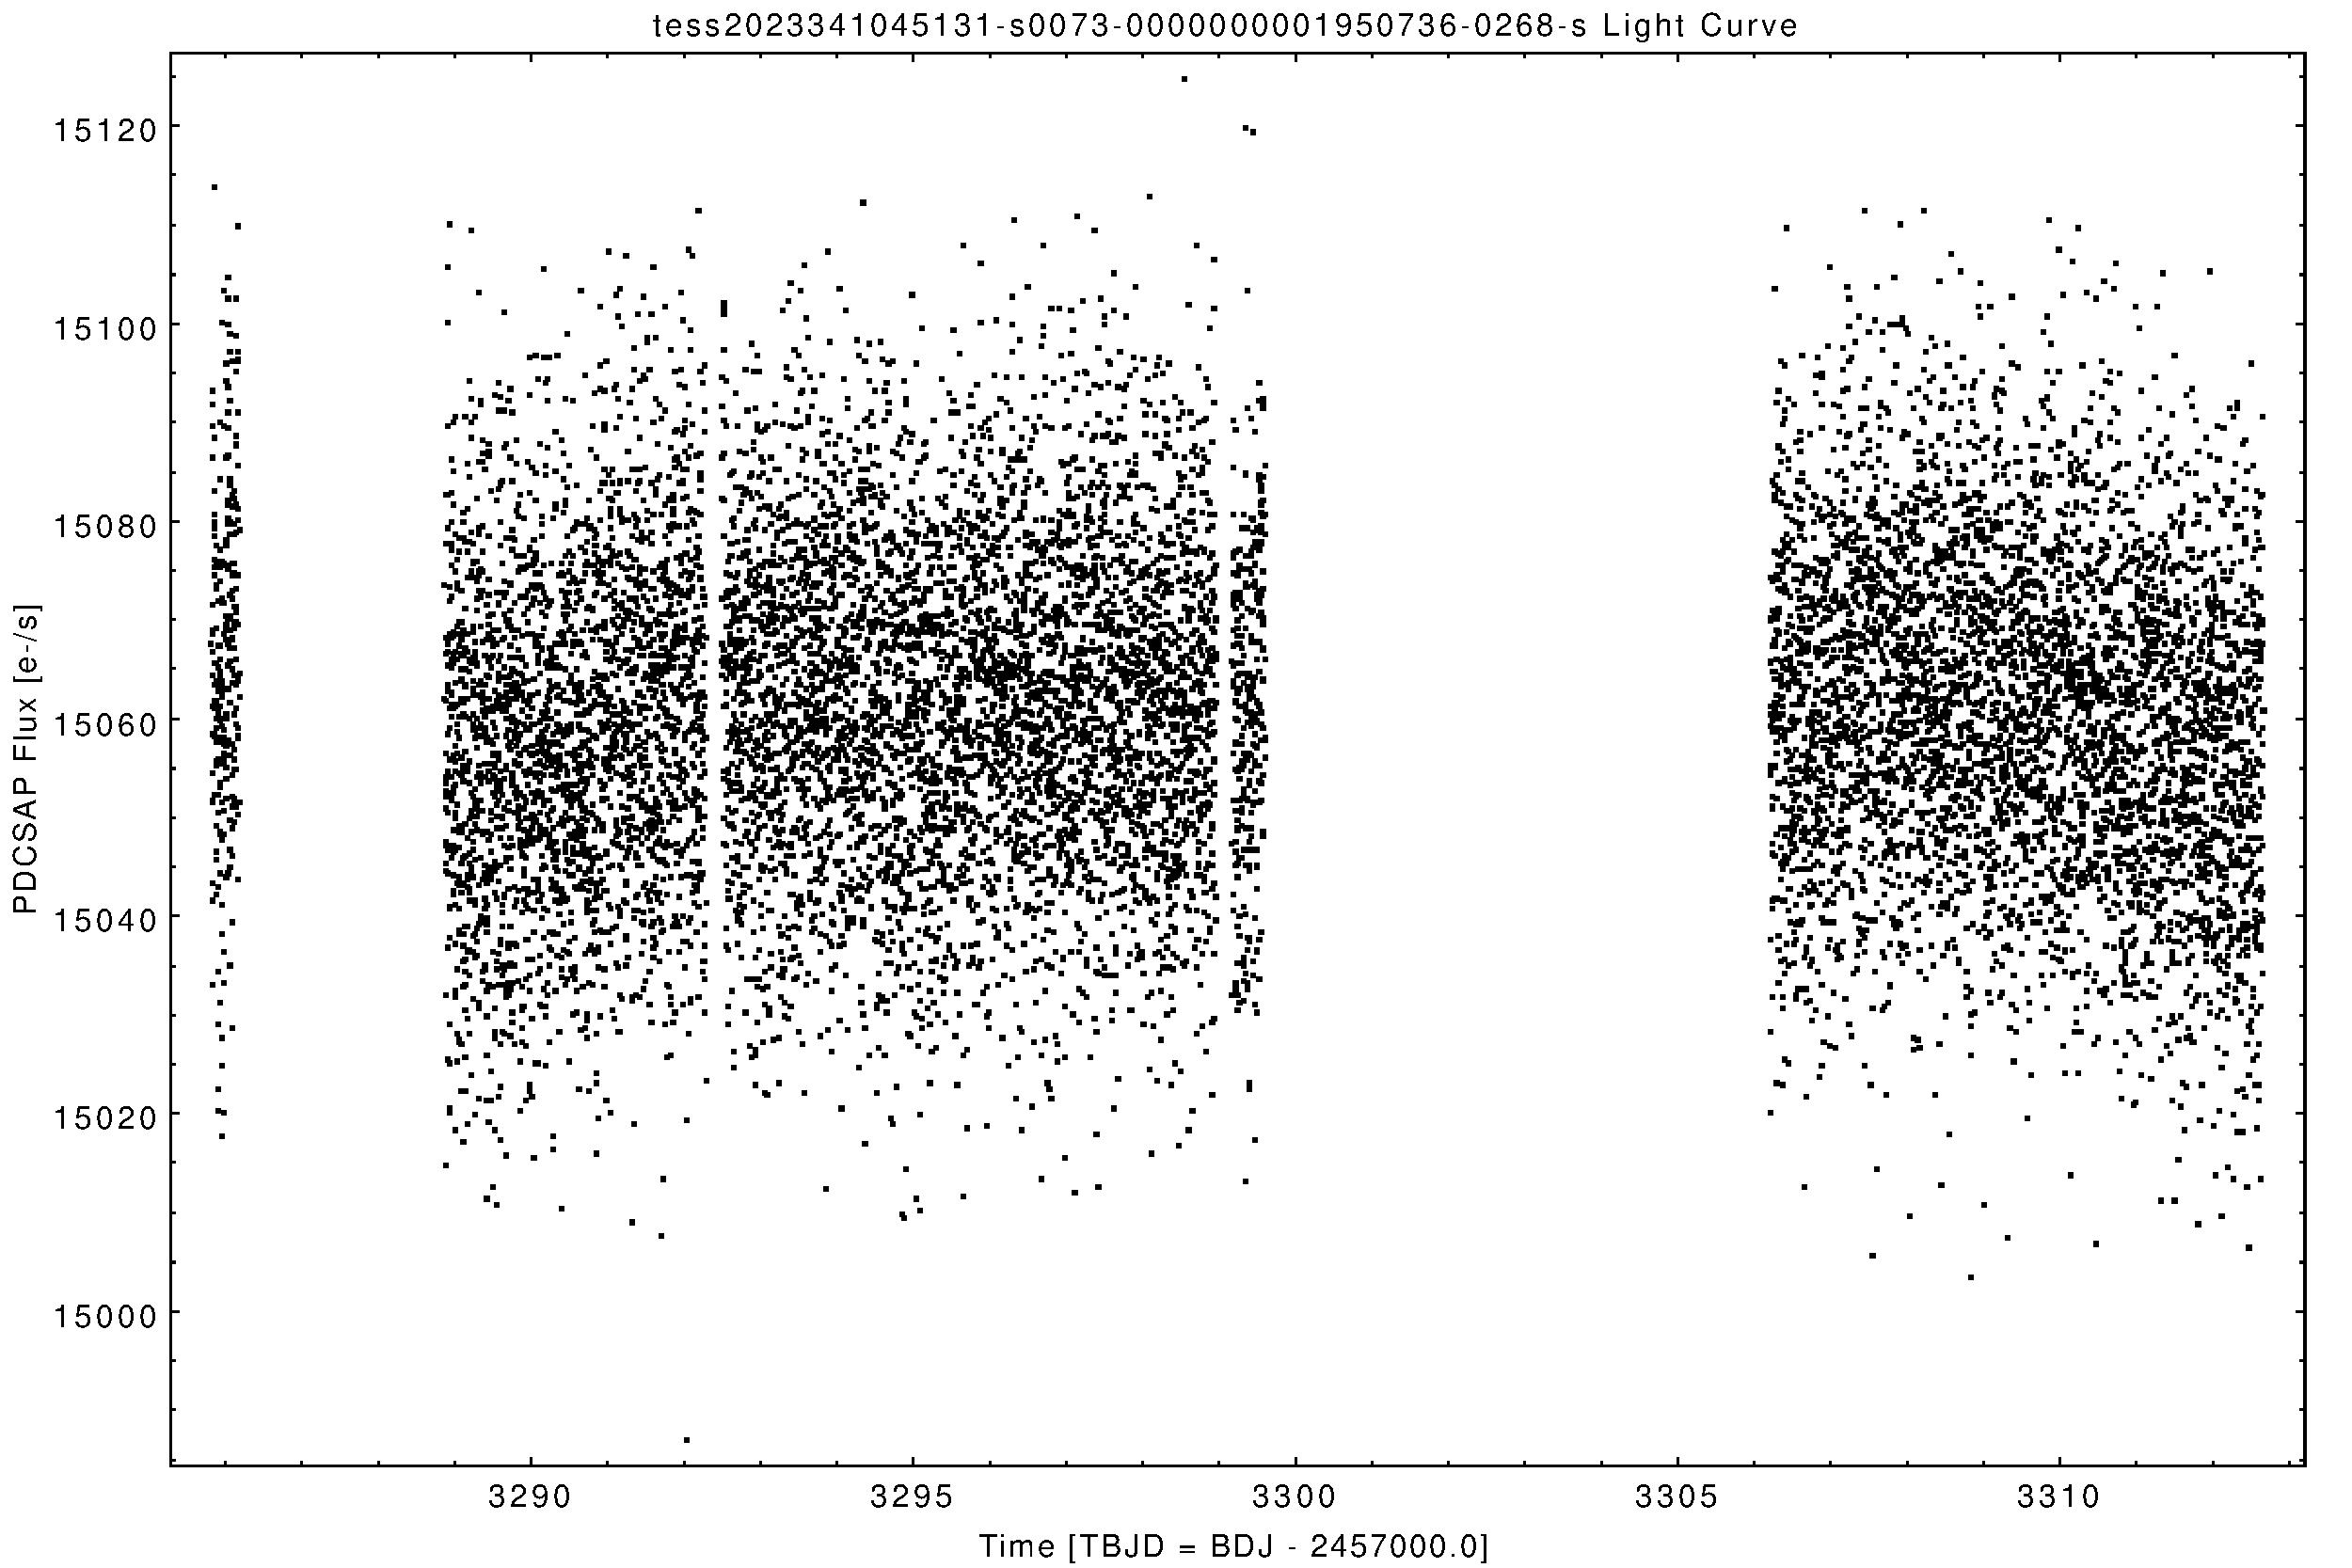
\includegraphics[width = 1\textwidth]{
      lightcurves/tess2023341045131-s0073-0000000001950736-0268-s.pdf}
    \caption{tess2023341045131-s0073-0000000001950736-0268-s light curve}
\end{figure}
\begin{figure}[htbp]
    \centering
    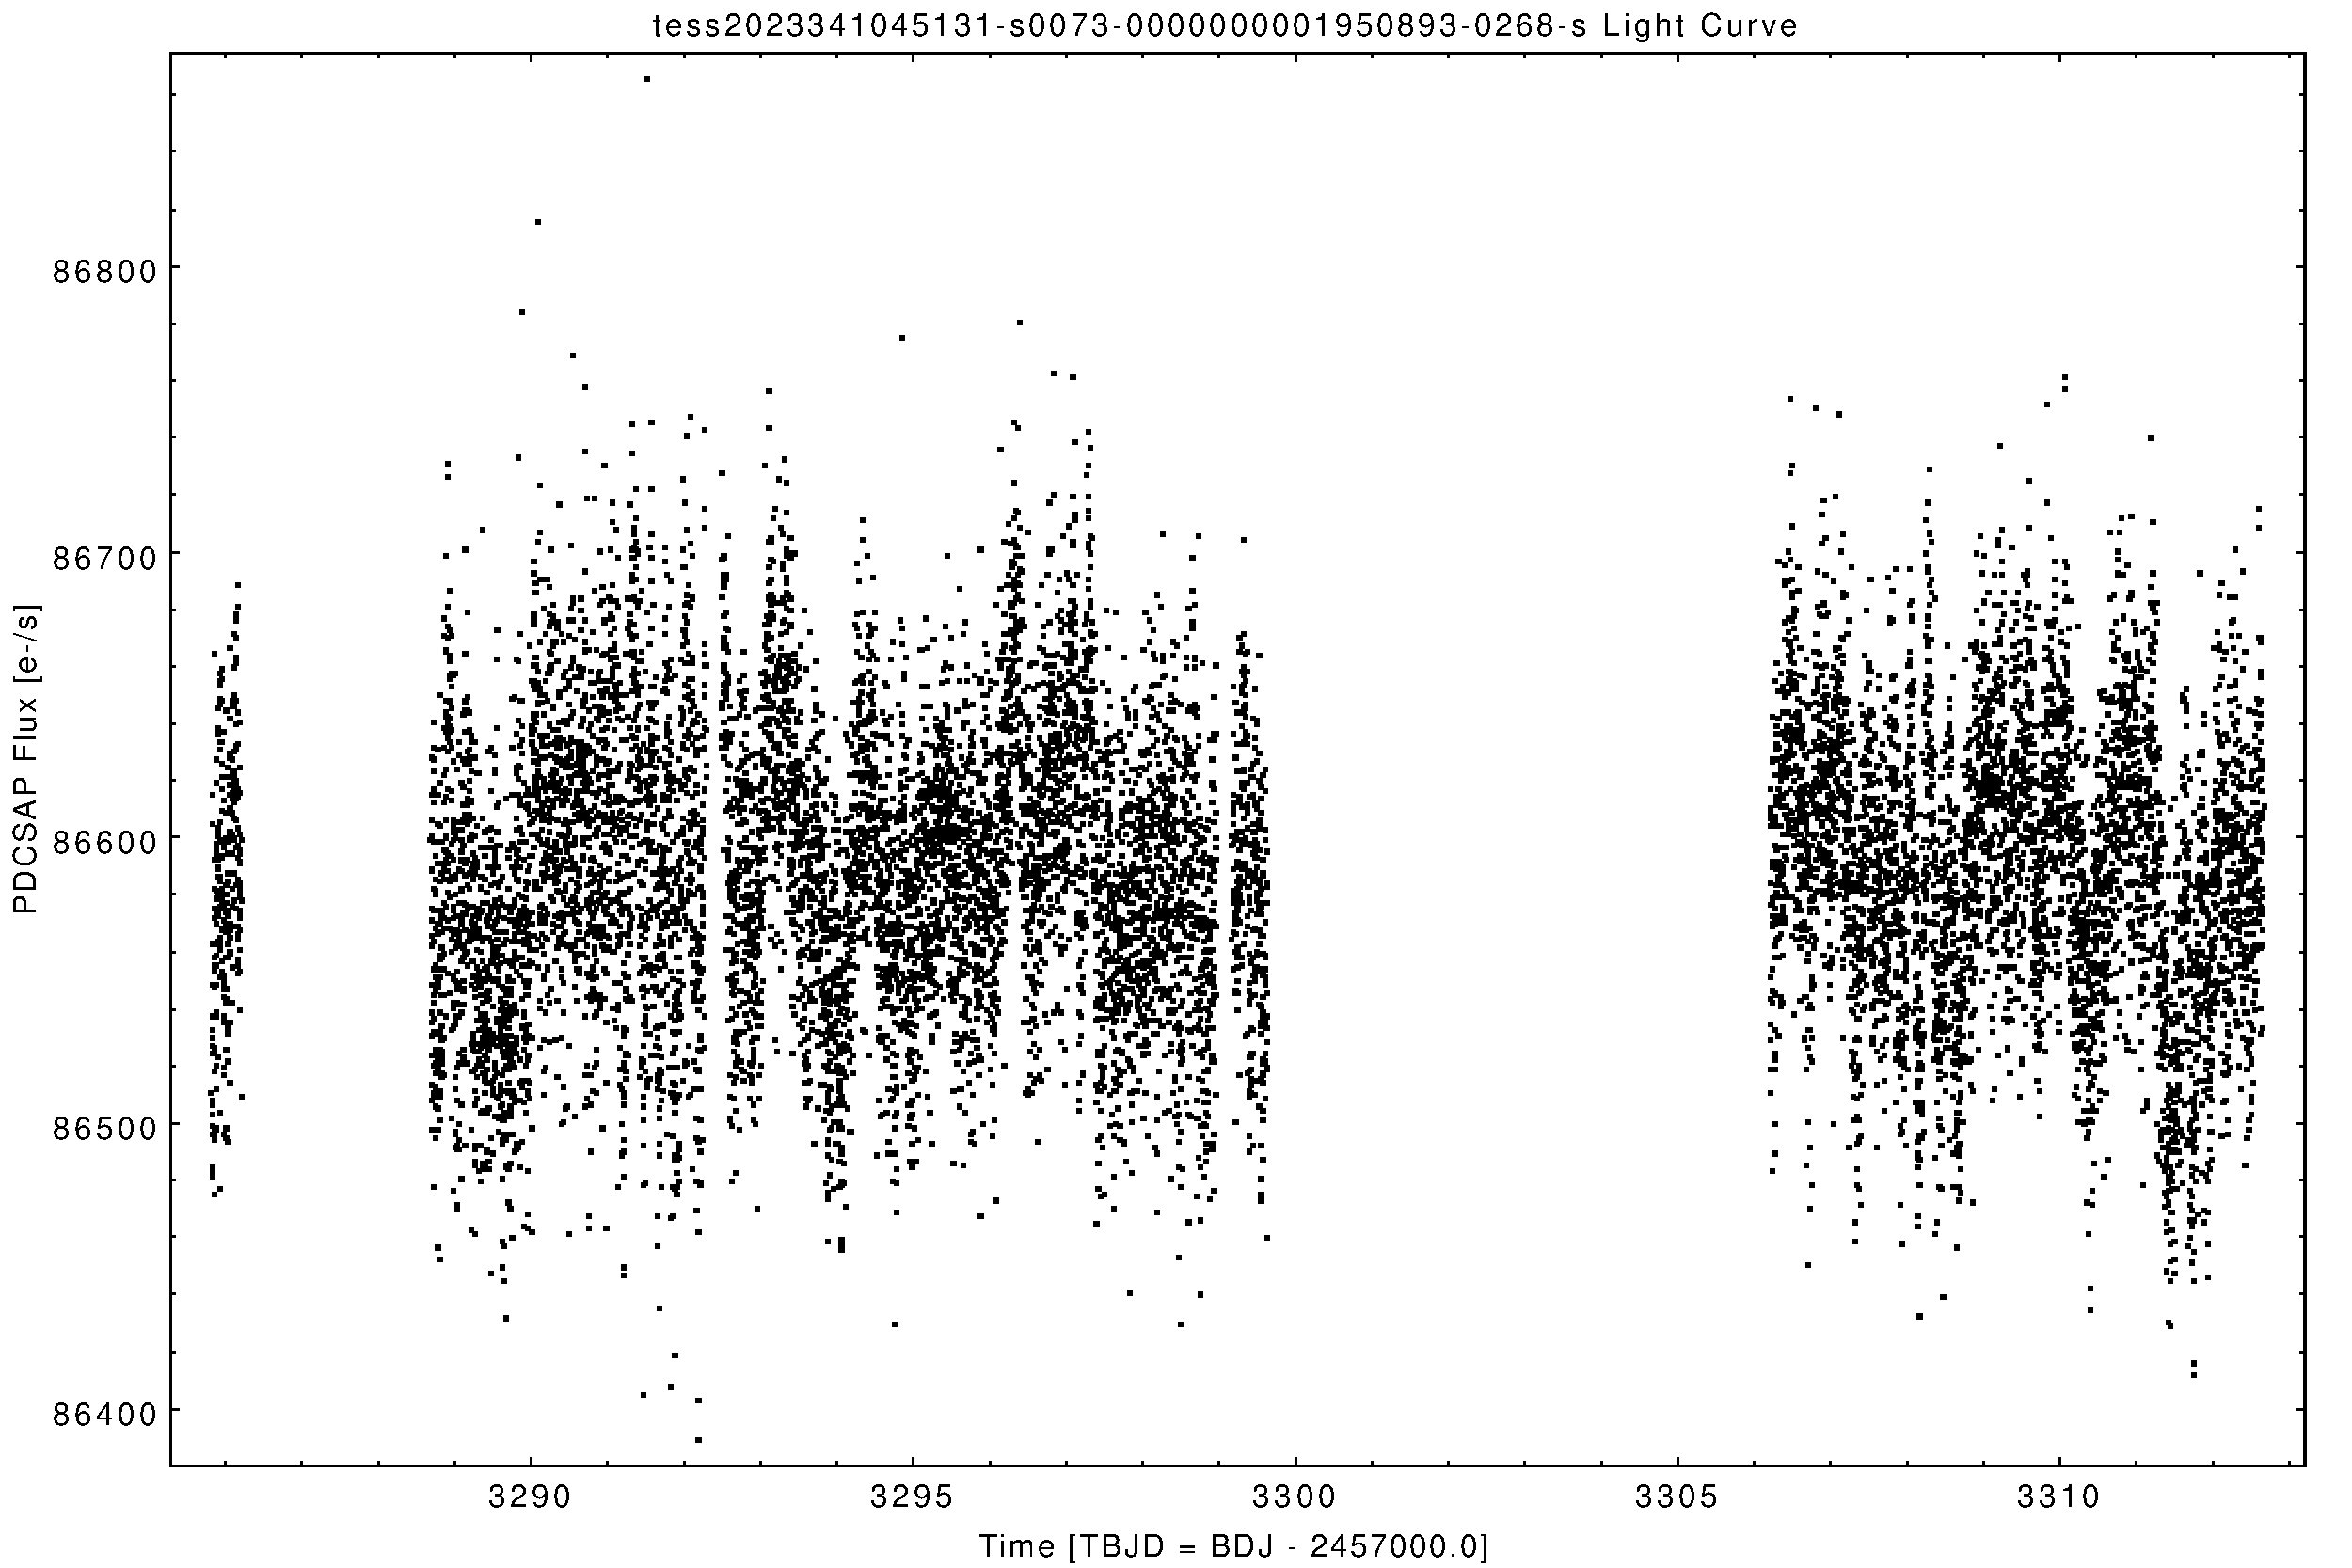
\includegraphics[width = 1\textwidth]{
      lightcurves/tess2023341045131-s0073-0000000001950893-0268-s.pdf}
    \caption{tess2023341045131-s0073-0000000001950893-0268-s light curve}
\end{figure}
\begin{figure}[htbp]
    \centering
    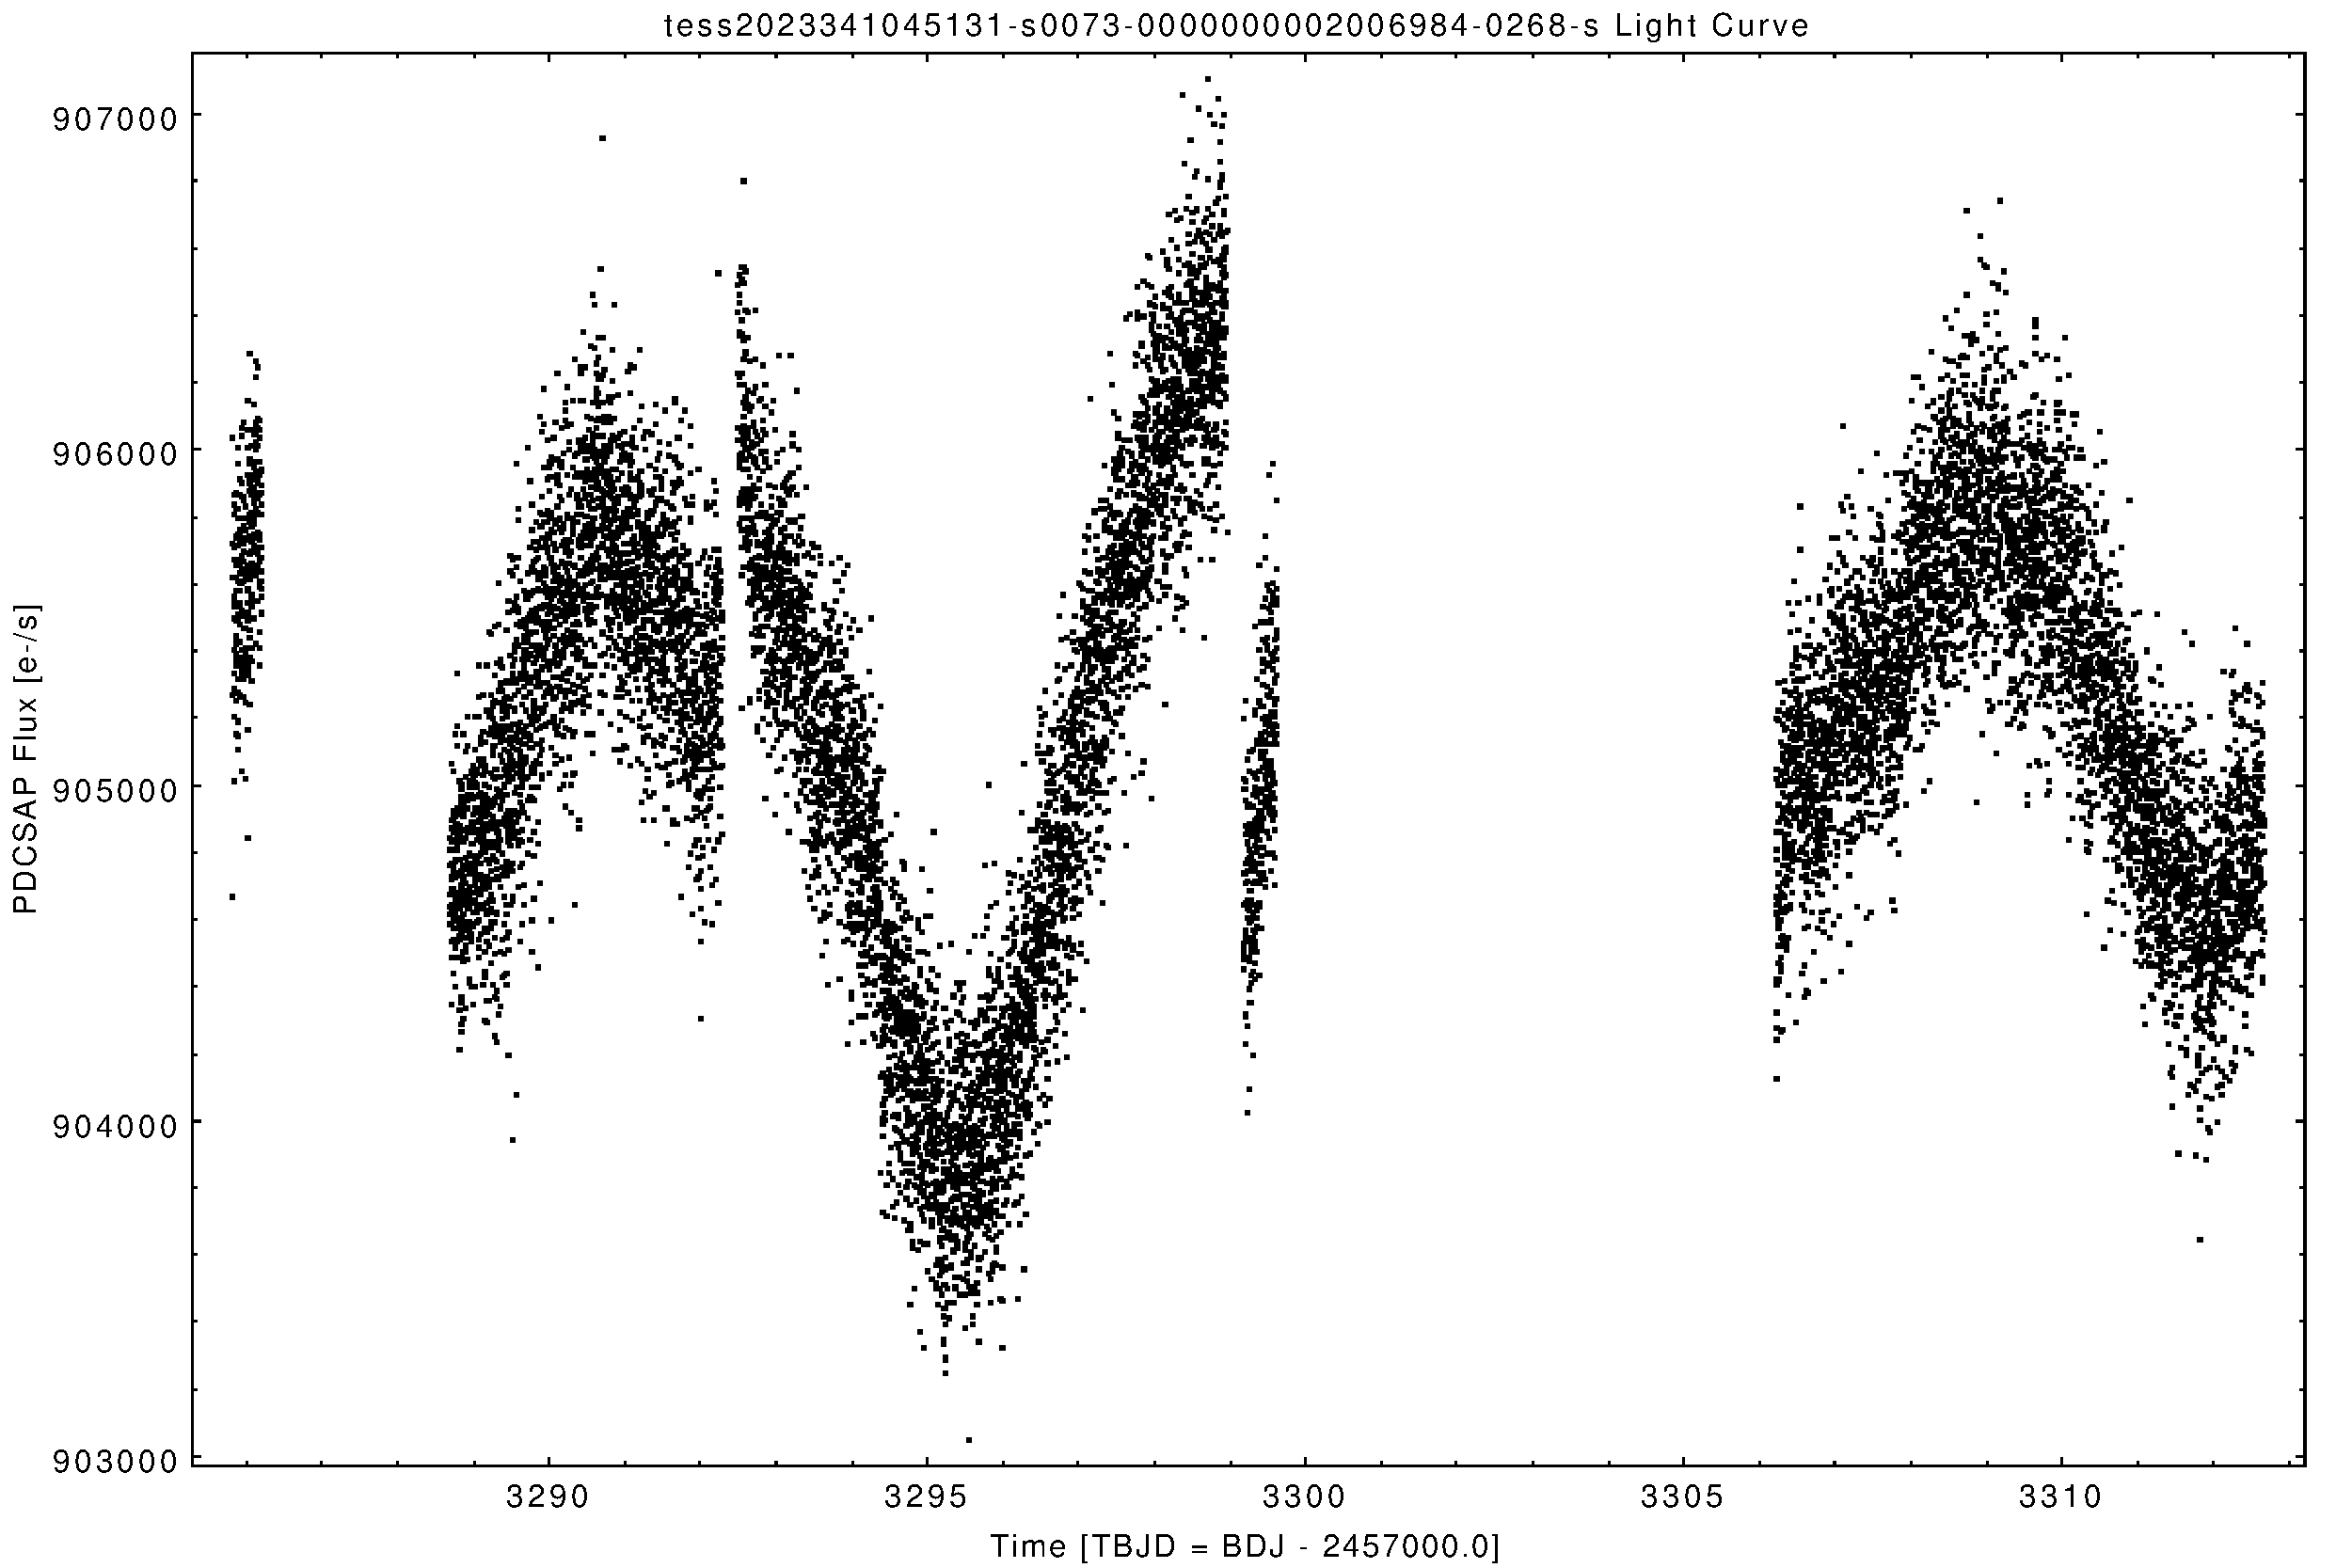
\includegraphics[width = 1\textwidth]{
      lightcurves/tess2023341045131-s0073-0000000002006984-0268-s.pdf}
    \caption{tess2023341045131-s0073-0000000002006984-0268-s light curve}
\end{figure}
\begin{figure}[htbp]
    \centering
    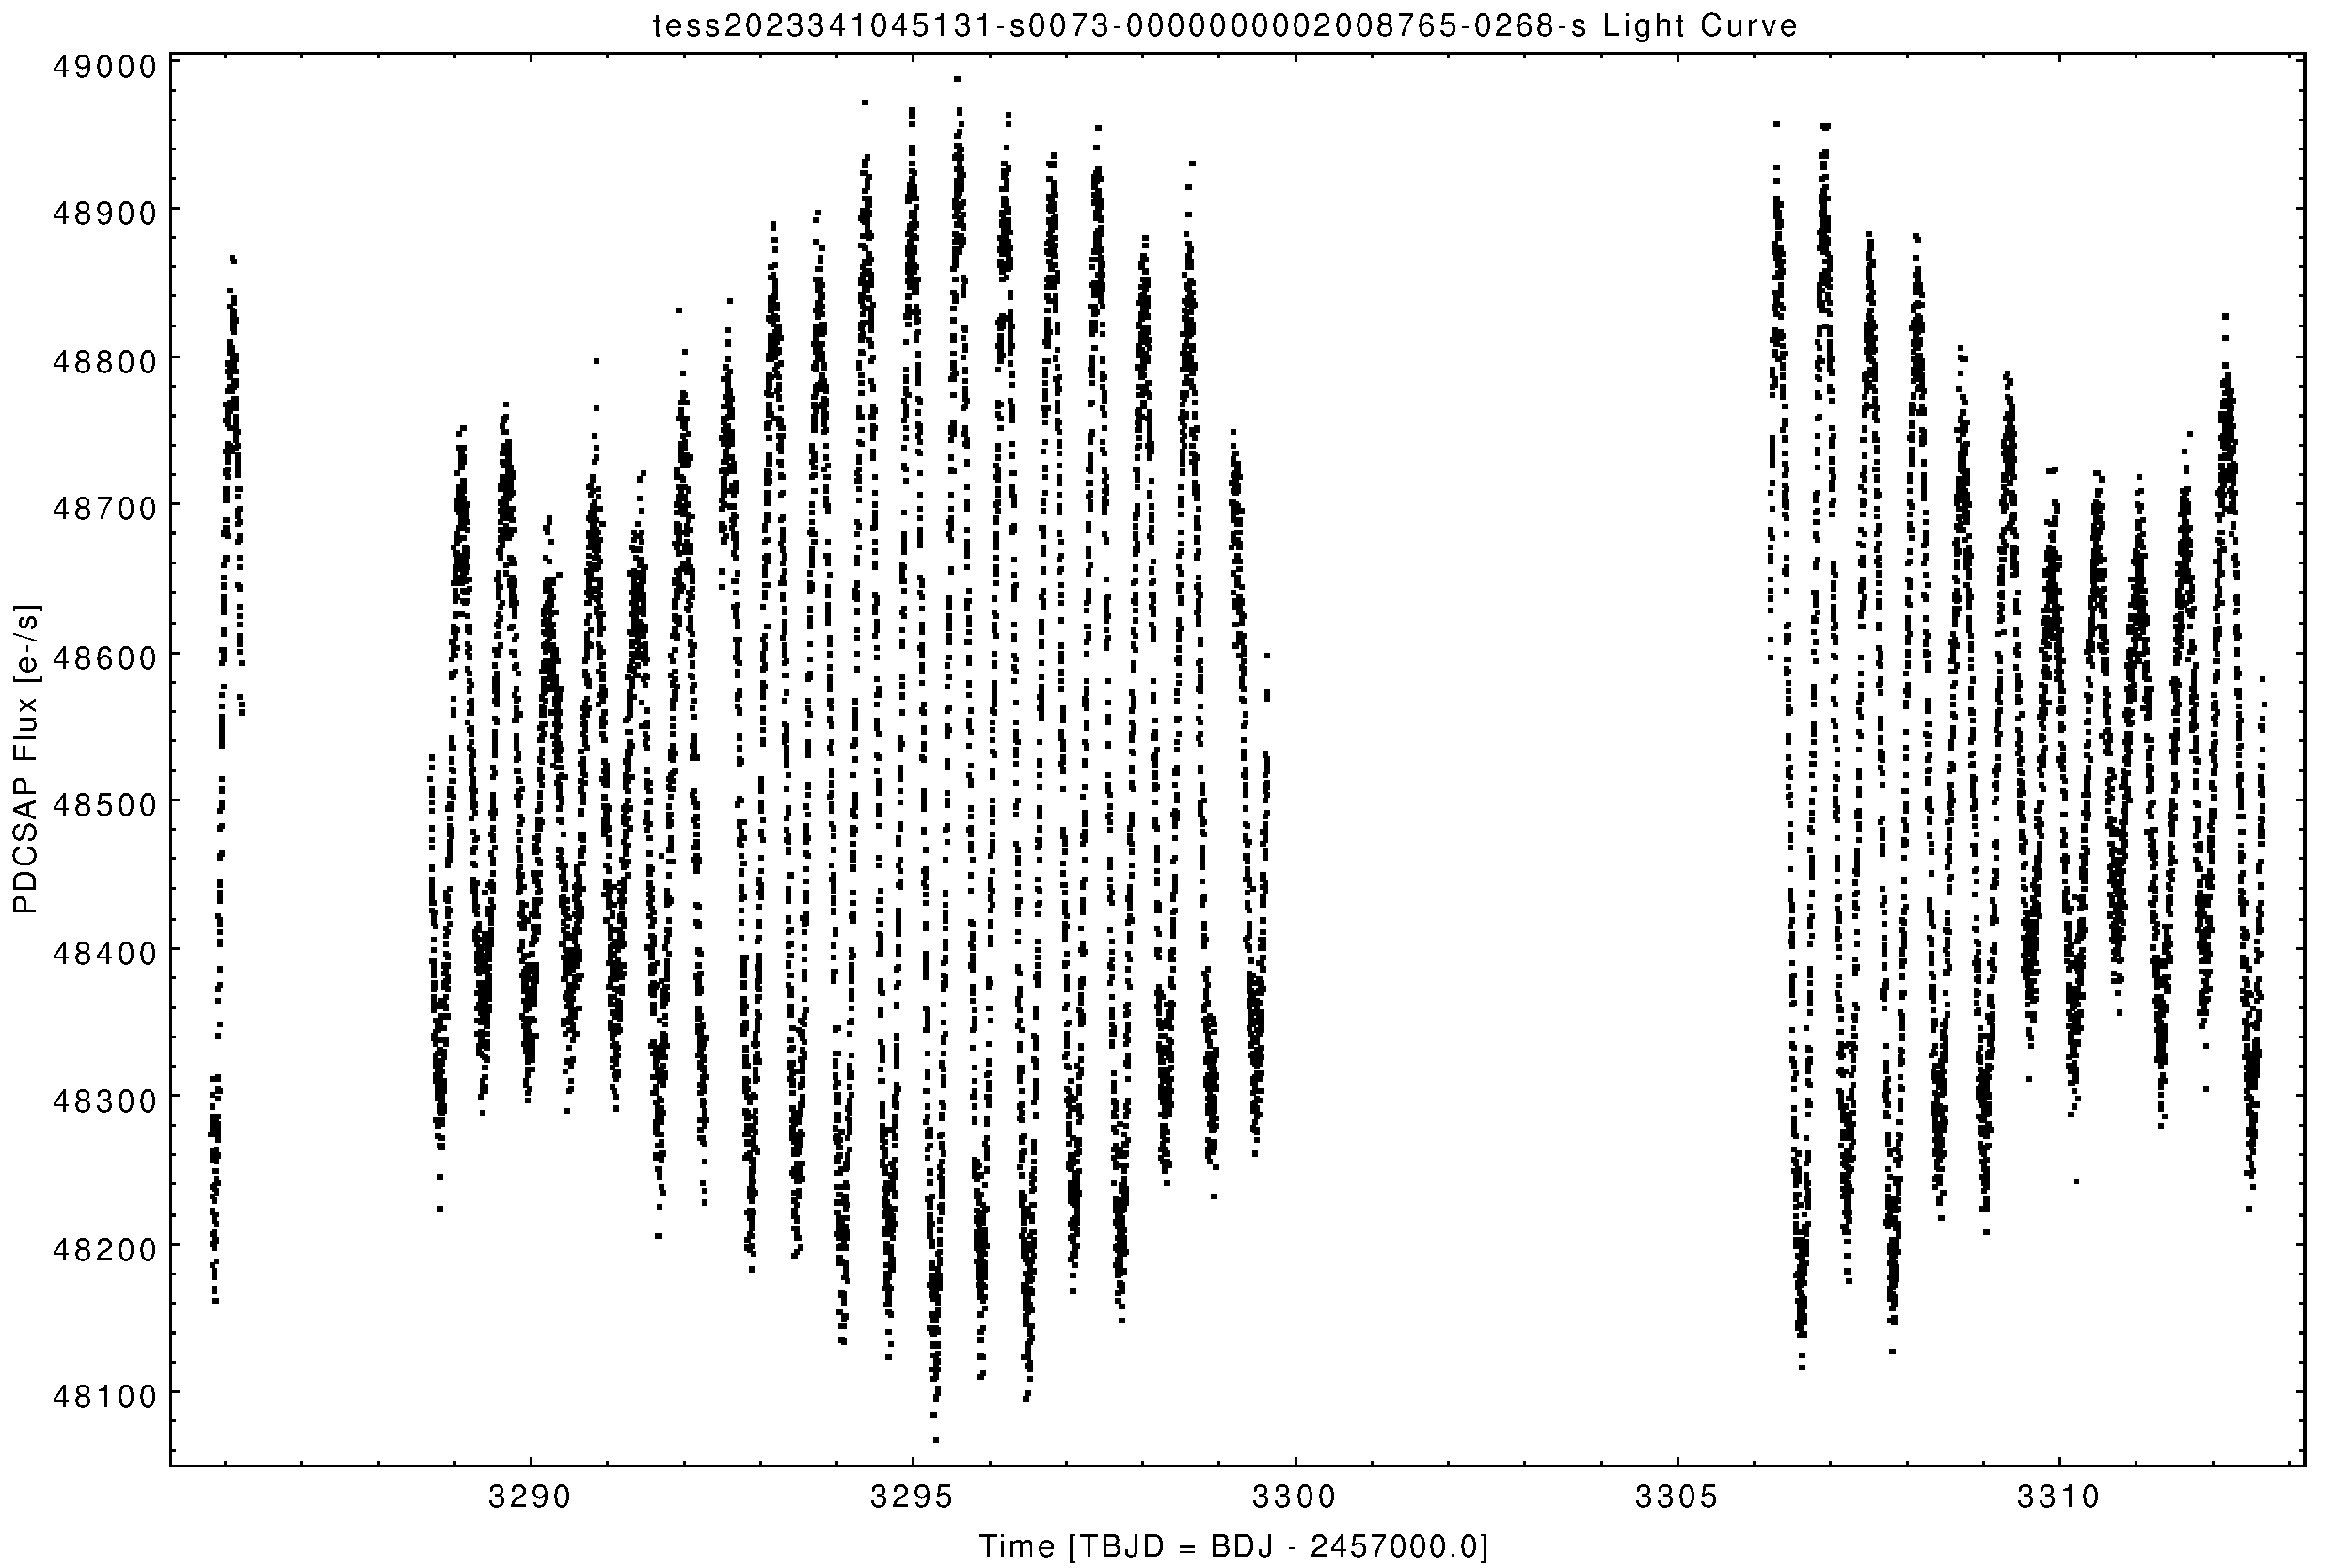
\includegraphics[width = 1\textwidth]{
      lightcurves/tess2023341045131-s0073-0000000002008765-0268-s.pdf}
    \caption{tess2023341045131-s0073-0000000002008765-0268-s light curve}
\end{figure}
\begin{figure}[htbp]
    \centering
    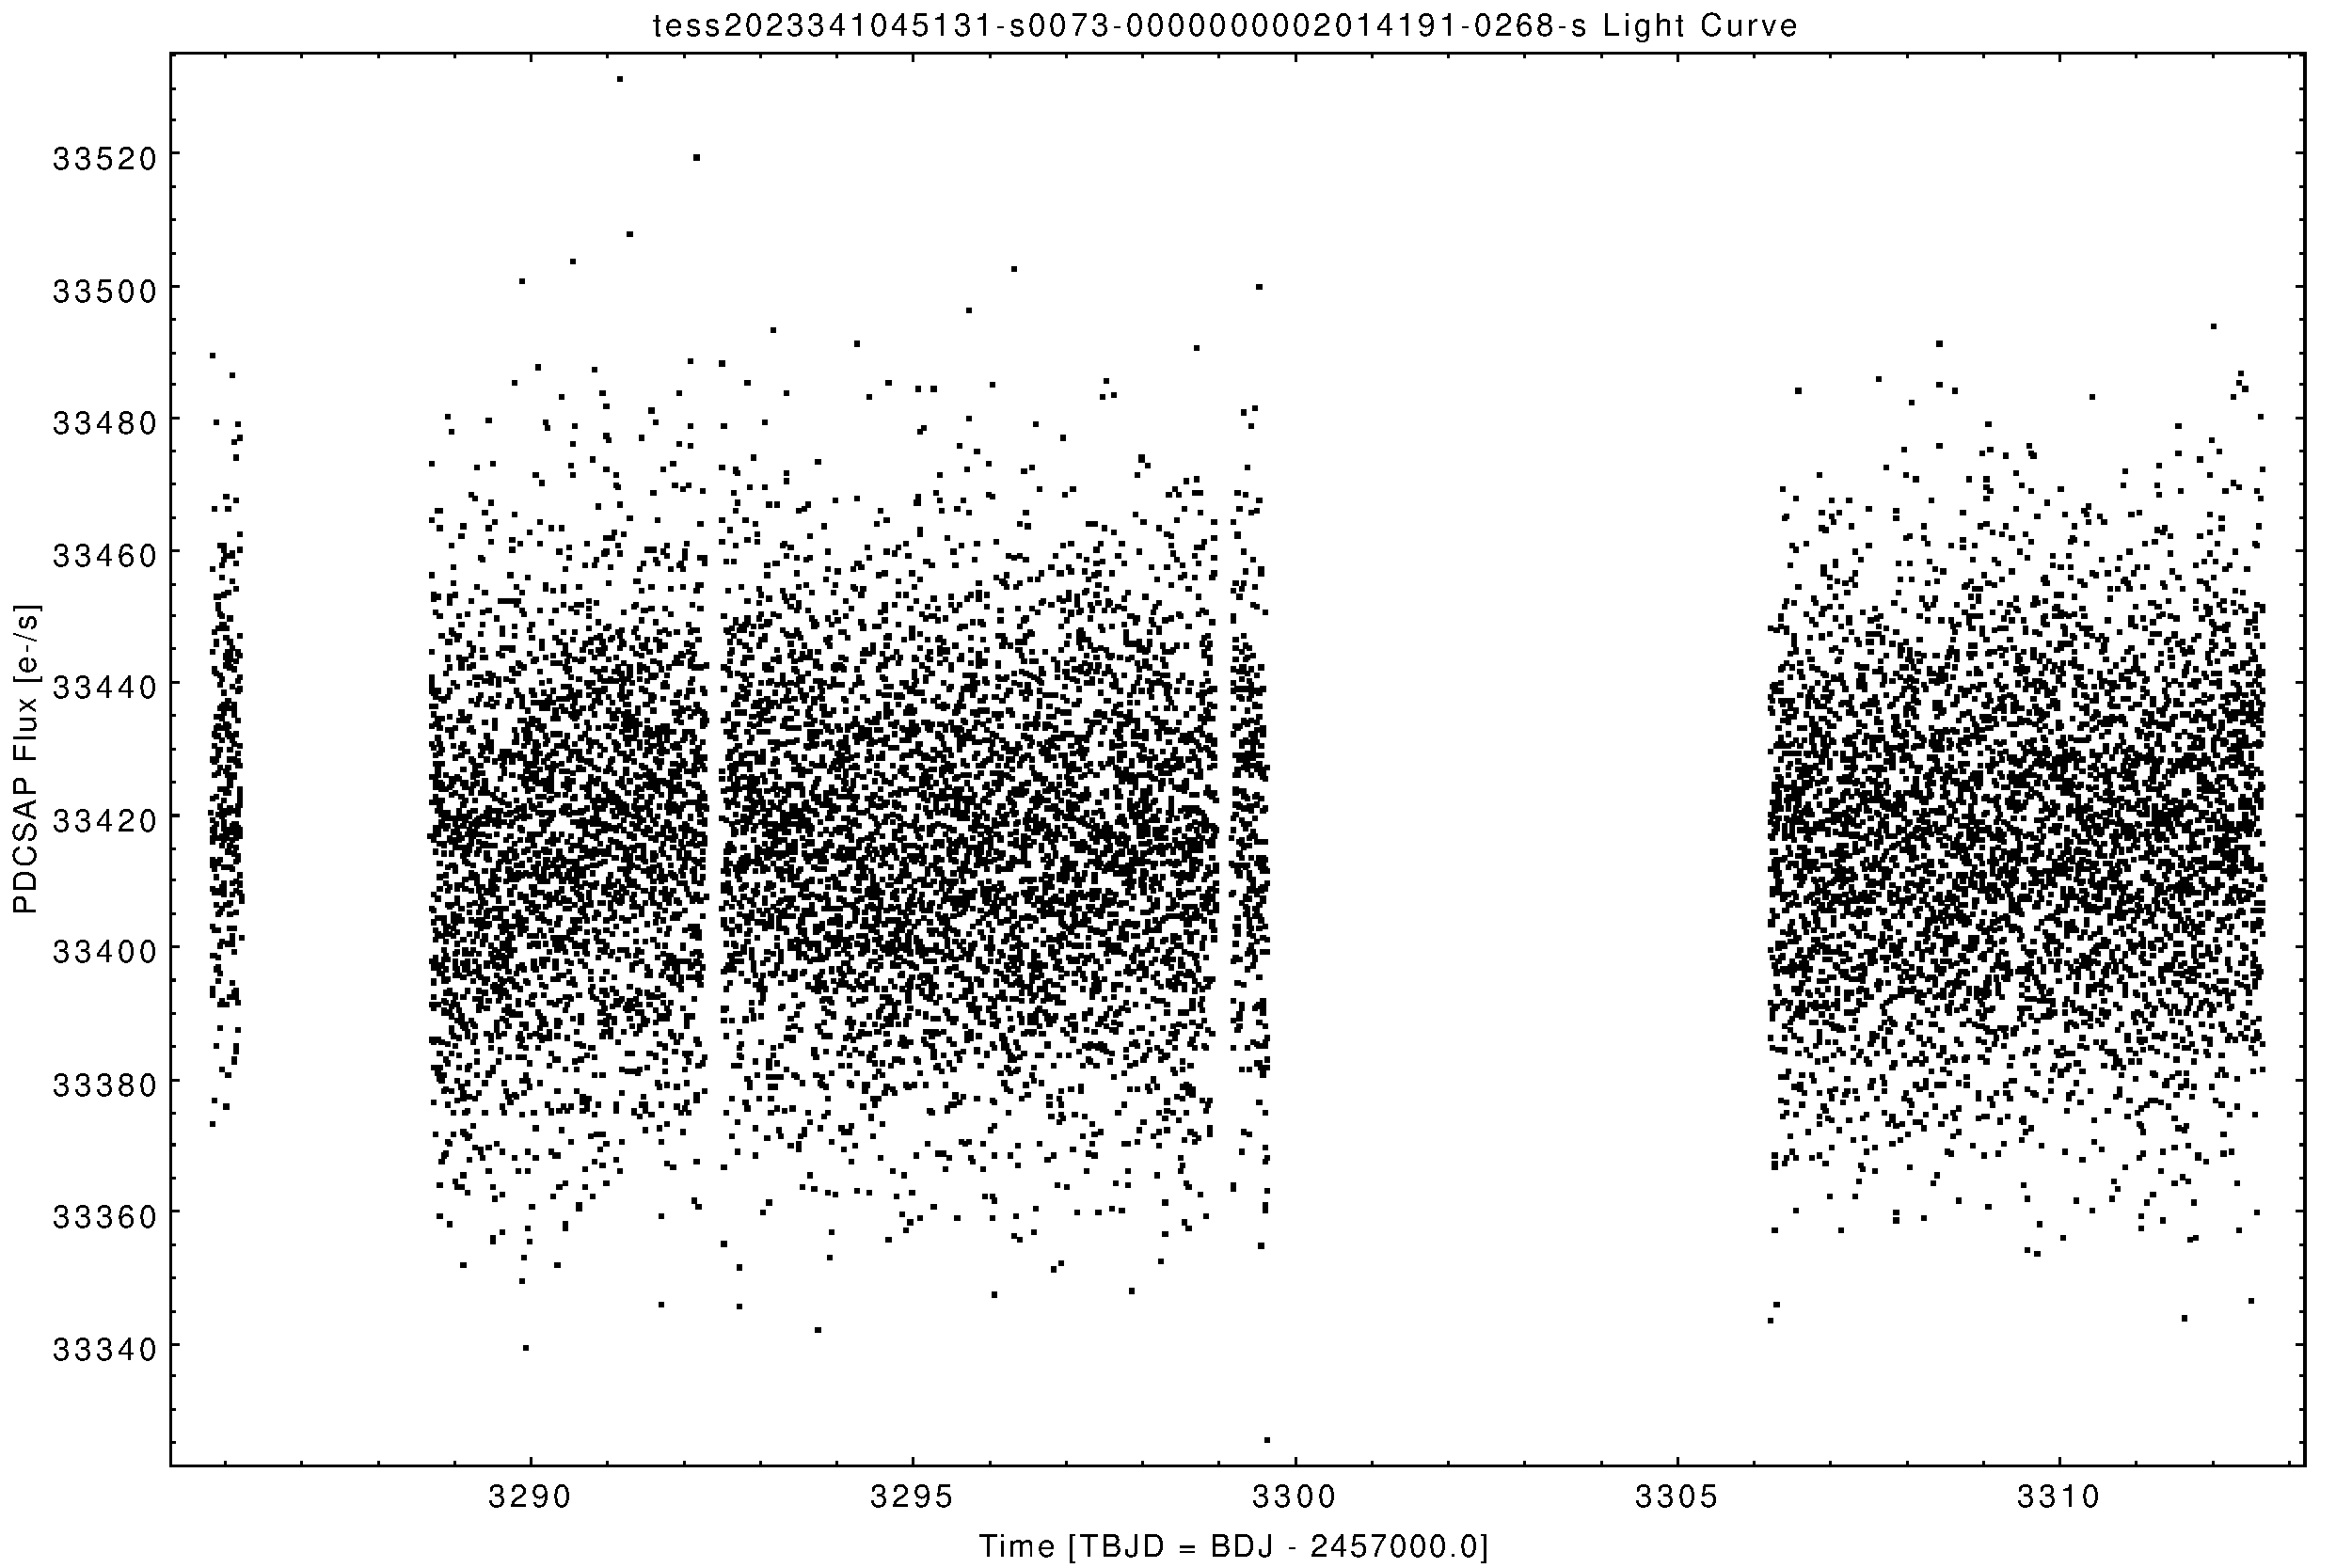
\includegraphics[width = 1\textwidth]{
      lightcurves/tess2023341045131-s0073-0000000002014191-0268-s.pdf}
    \caption{tess2023341045131-s0073-0000000002014191-0268-s light curve}
\end{figure}
\begin{figure}[htbp]
    \centering
    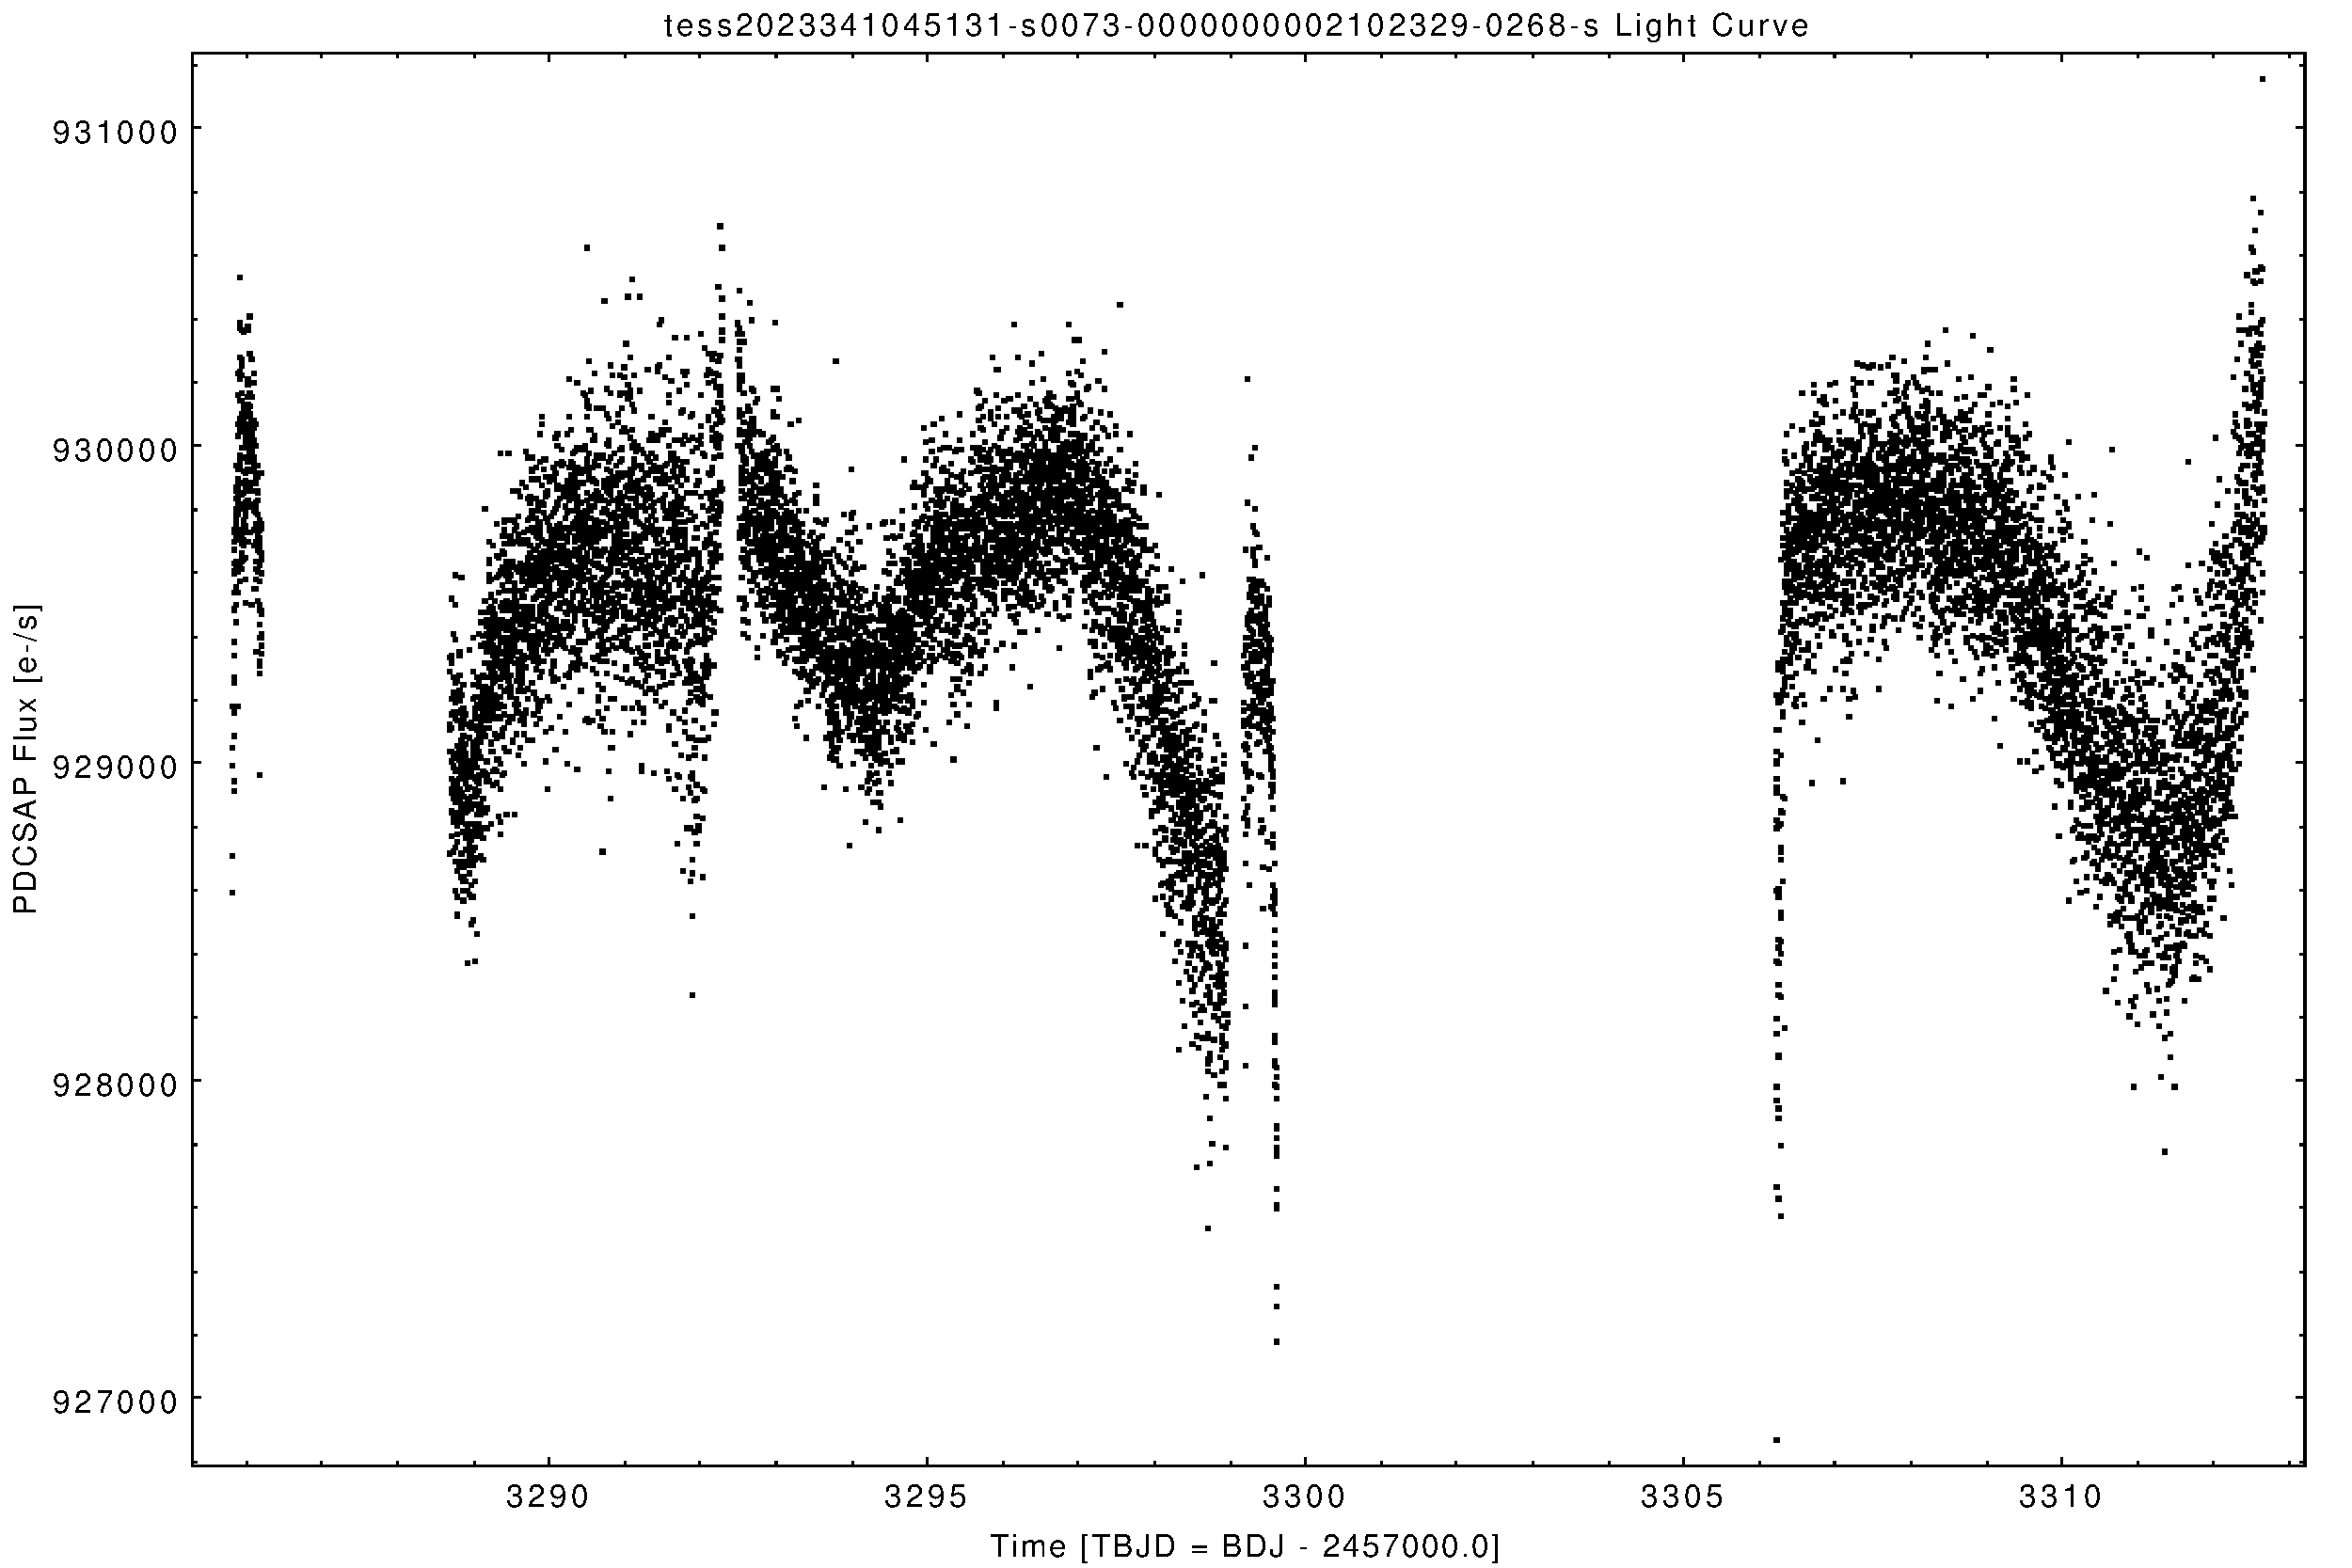
\includegraphics[width = 1\textwidth]{
      lightcurves/tess2023341045131-s0073-0000000002102329-0268-s.pdf}
    \caption{tess2023341045131-s0073-0000000002102329-0268-s light curve}
\end{figure}
\begin{figure}[htbp]
    \centering
    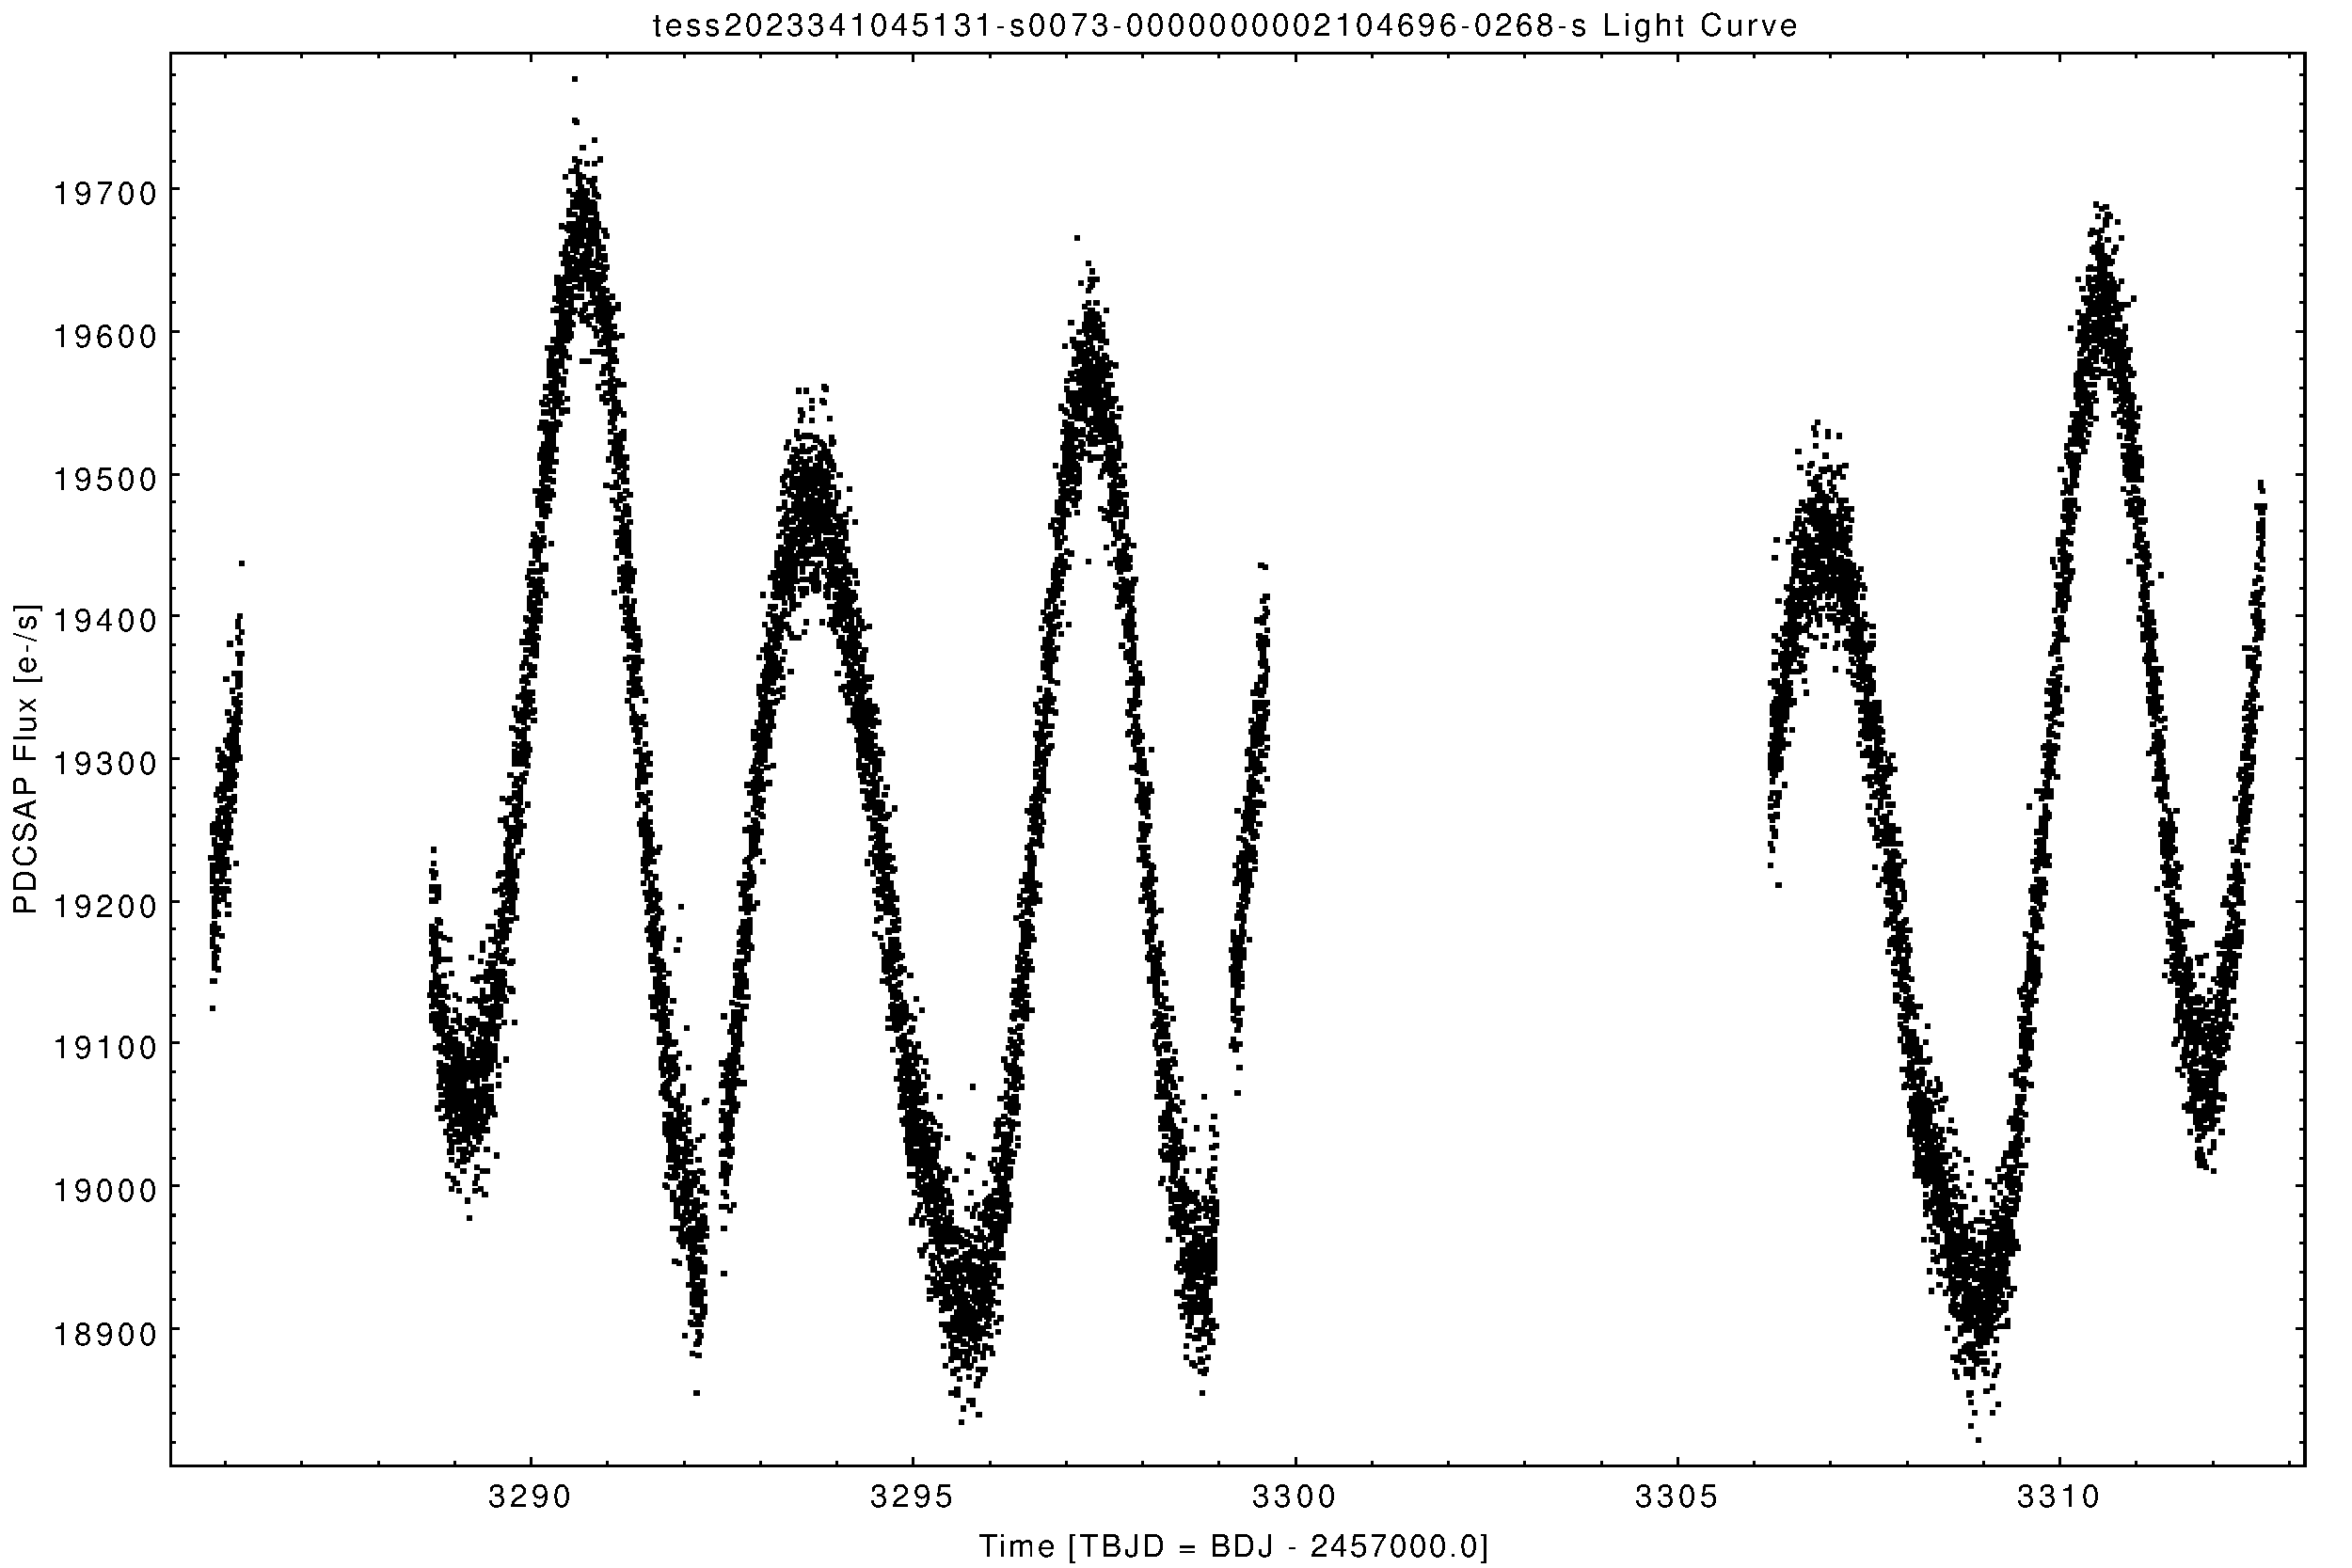
\includegraphics[width = 1\textwidth]{
      lightcurves/tess2023341045131-s0073-0000000002104696-0268-s.pdf}
    \caption{tess2023341045131-s0073-0000000002104696-0268-s light curve}
\end{figure}
\begin{figure}[htbp]
    \centering
    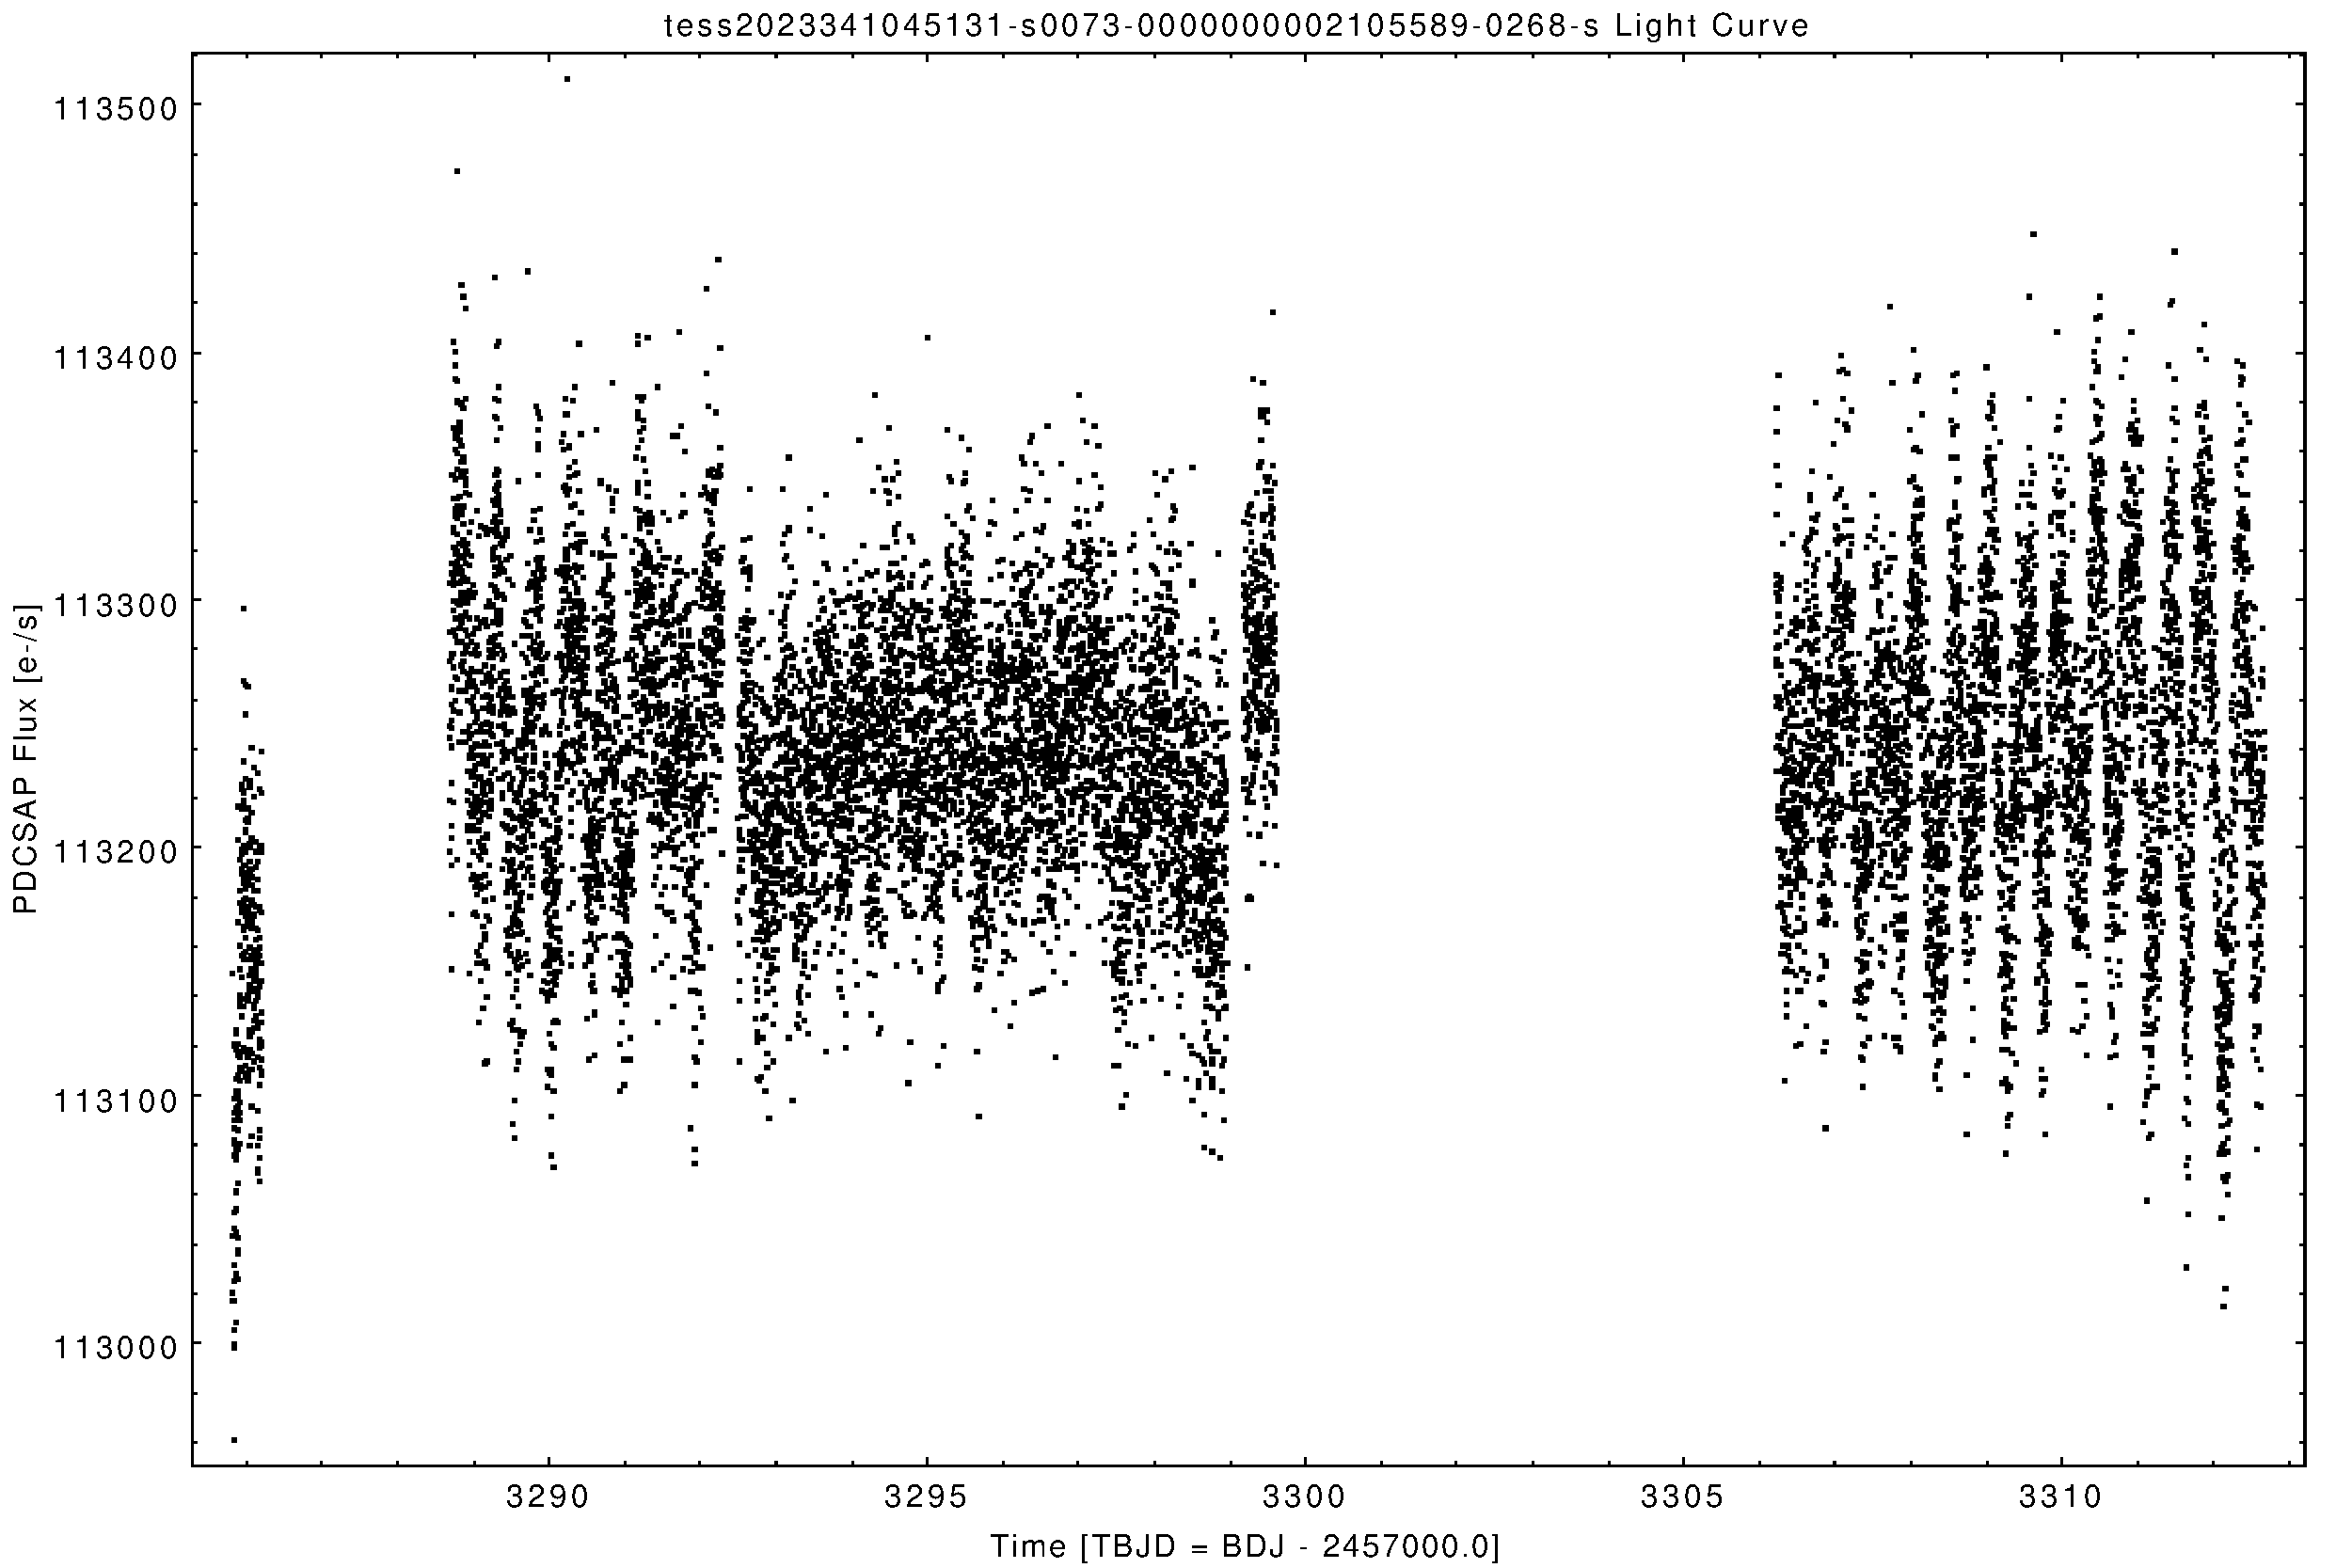
\includegraphics[width = 1\textwidth]{
      lightcurves/tess2023341045131-s0073-0000000002105589-0268-s.pdf}
    \caption{tess2023341045131-s0073-0000000002105589-0268-s light curve}
\end{figure}
\begin{figure}[htbp]
    \centering
    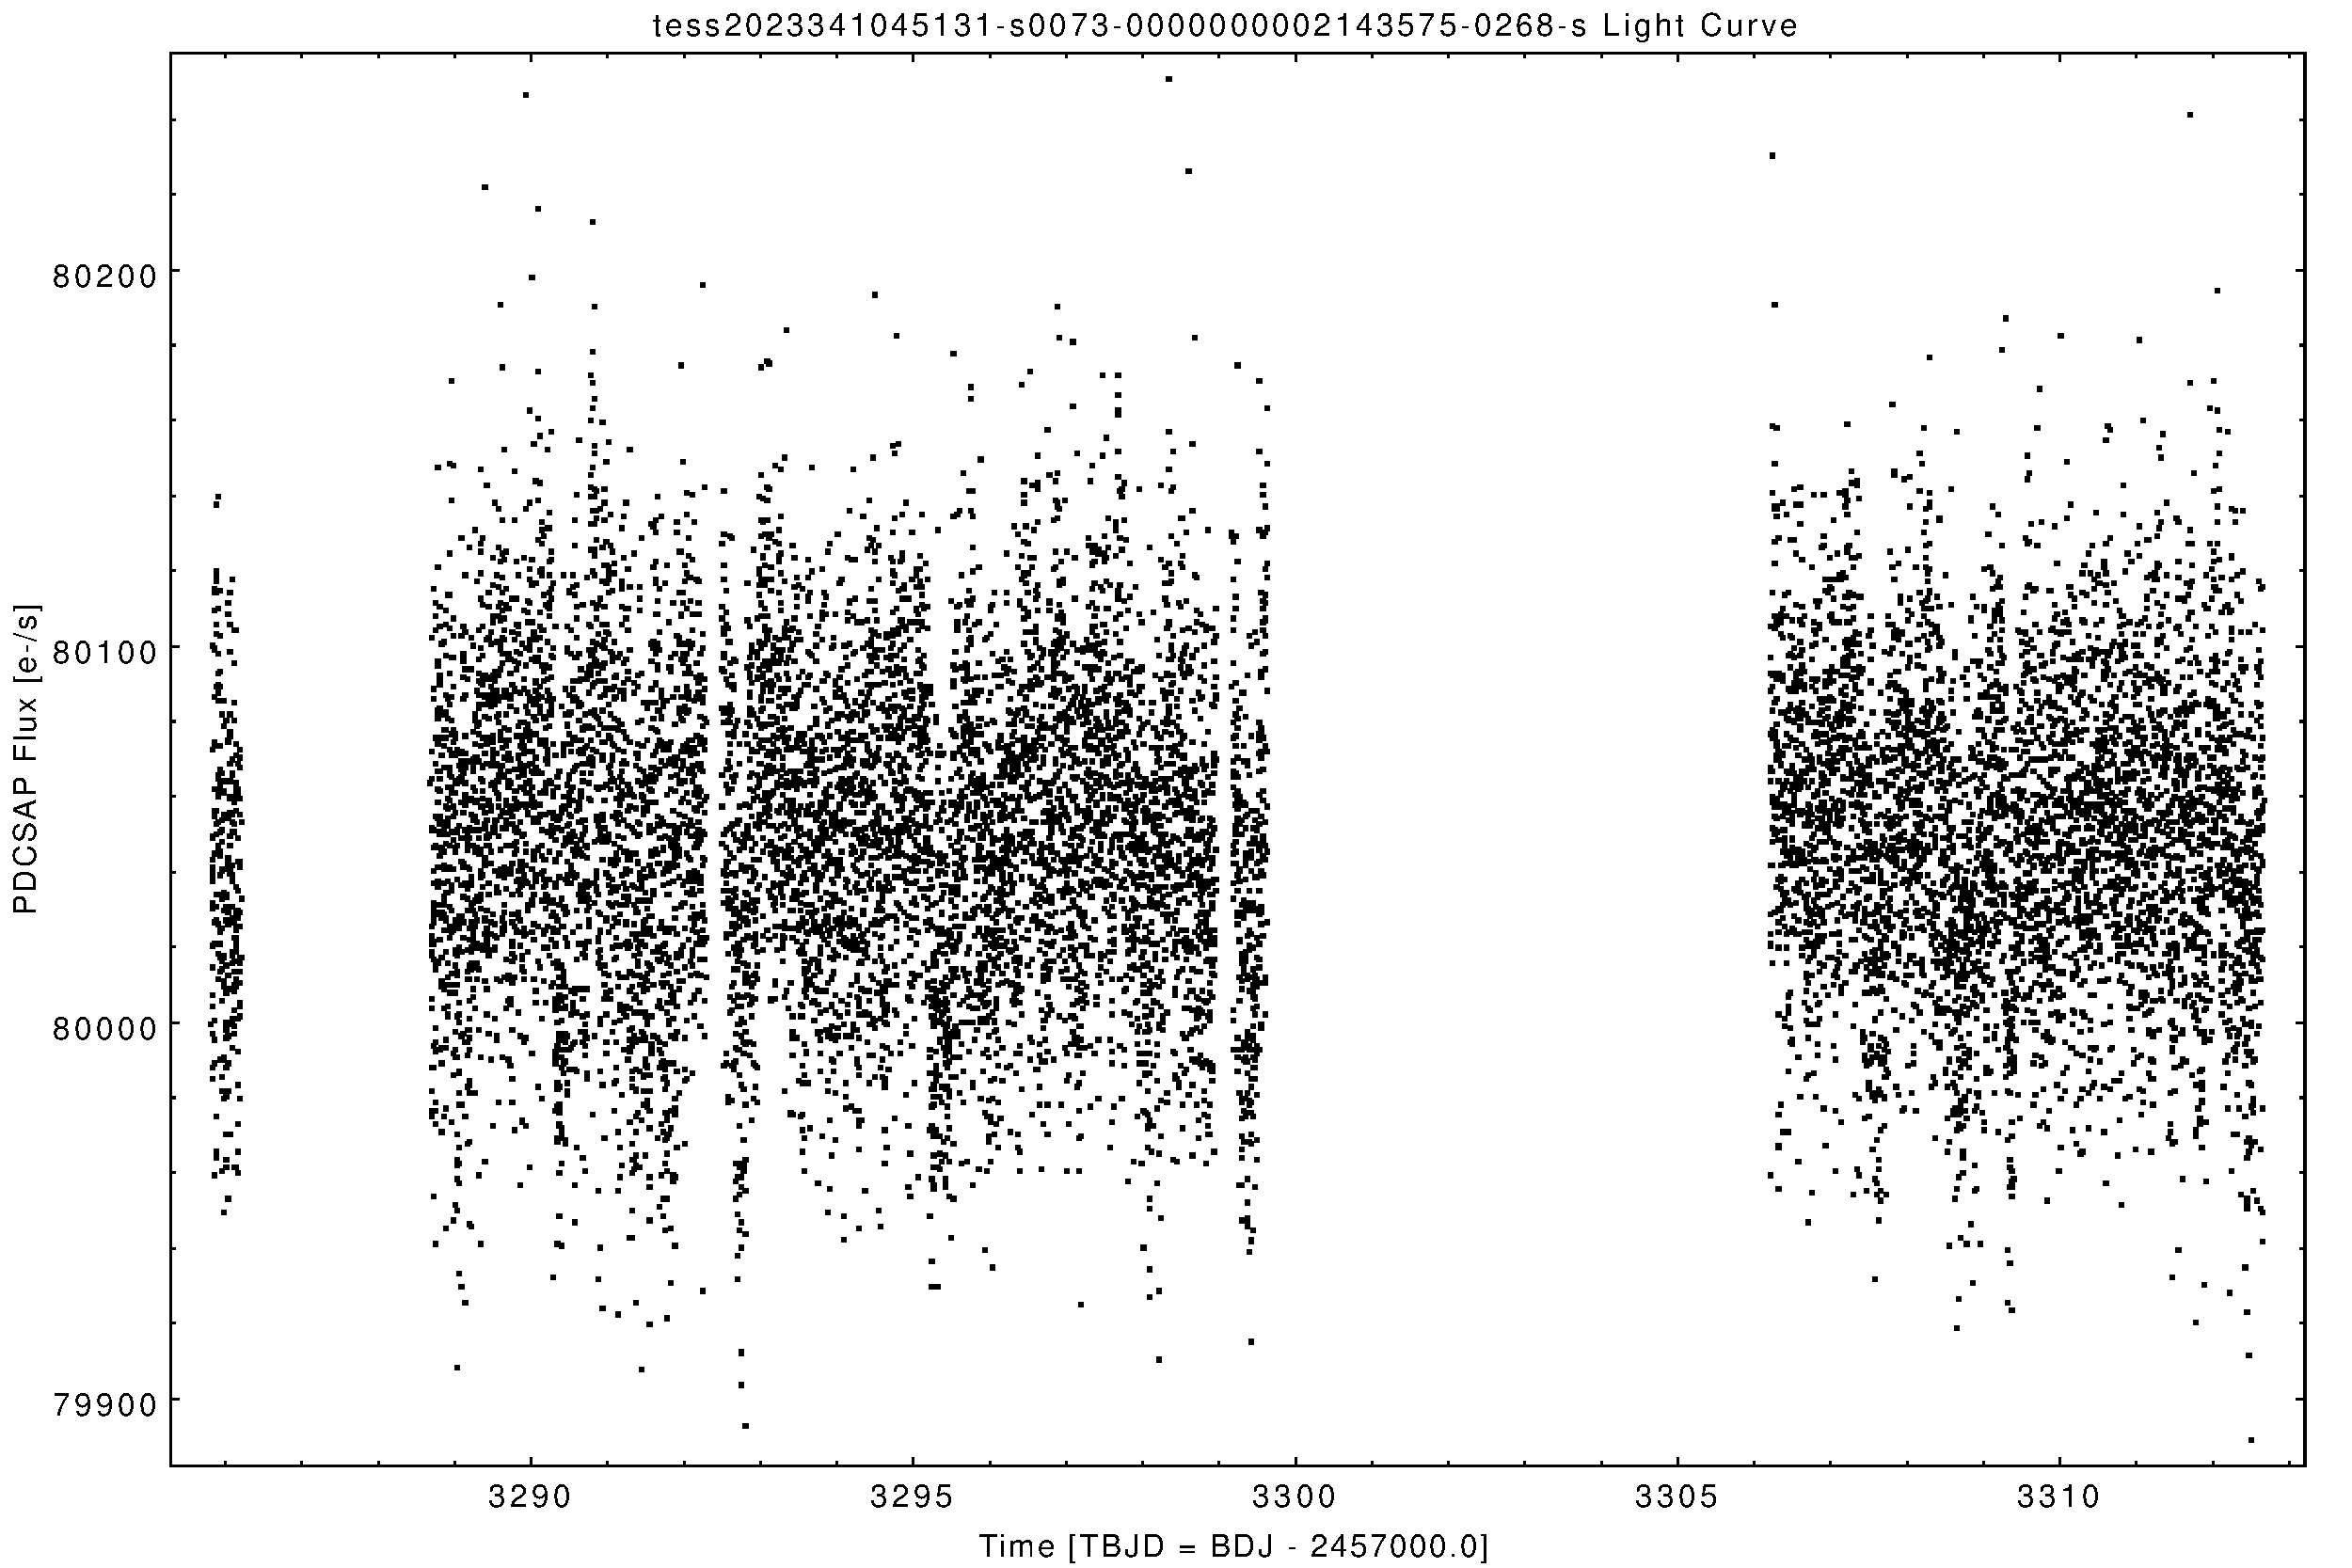
\includegraphics[width = 1\textwidth]{
      lightcurves/tess2023341045131-s0073-0000000002143575-0268-s.pdf}
    \caption{tess2023341045131-s0073-0000000002143575-0268-s light curve}
\end{figure}
\begin{figure}[htbp]
    \centering
    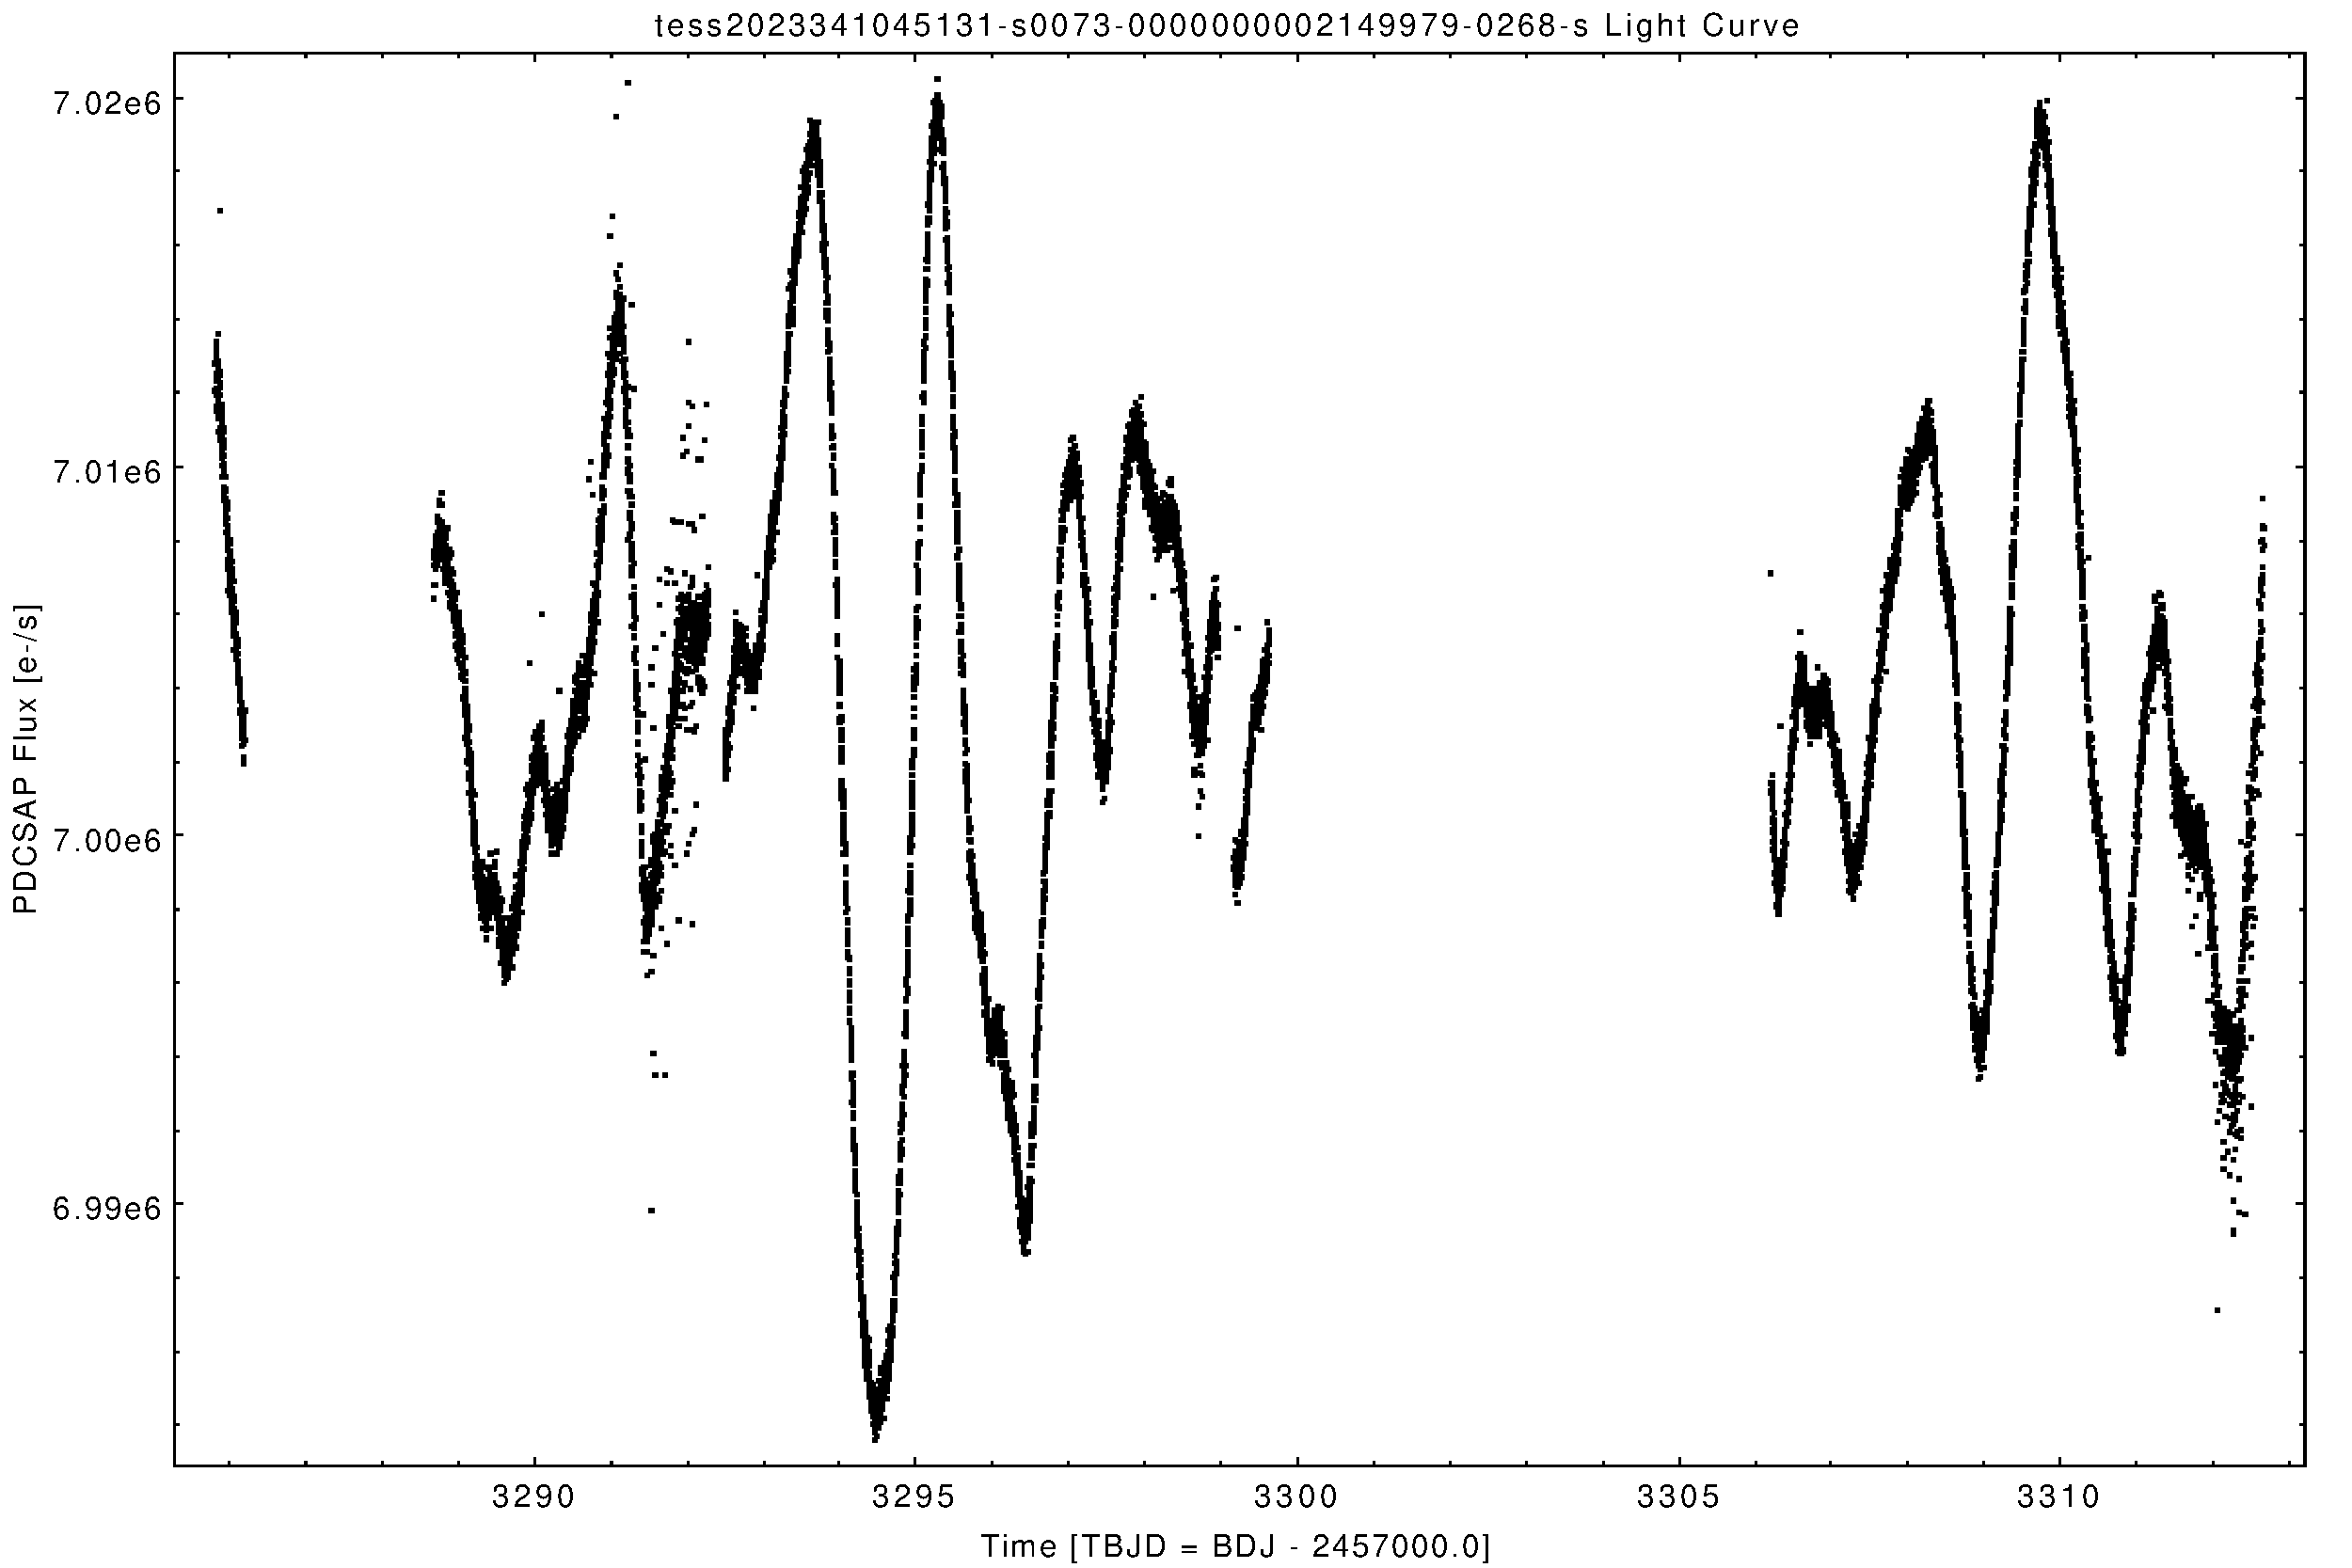
\includegraphics[width = 1\textwidth]{
      lightcurves/tess2023341045131-s0073-0000000002149979-0268-s.pdf}
    \caption{tess2023341045131-s0073-0000000002149979-0268-s light curve}
\end{figure}
\begin{figure}[htbp]
    \centering
    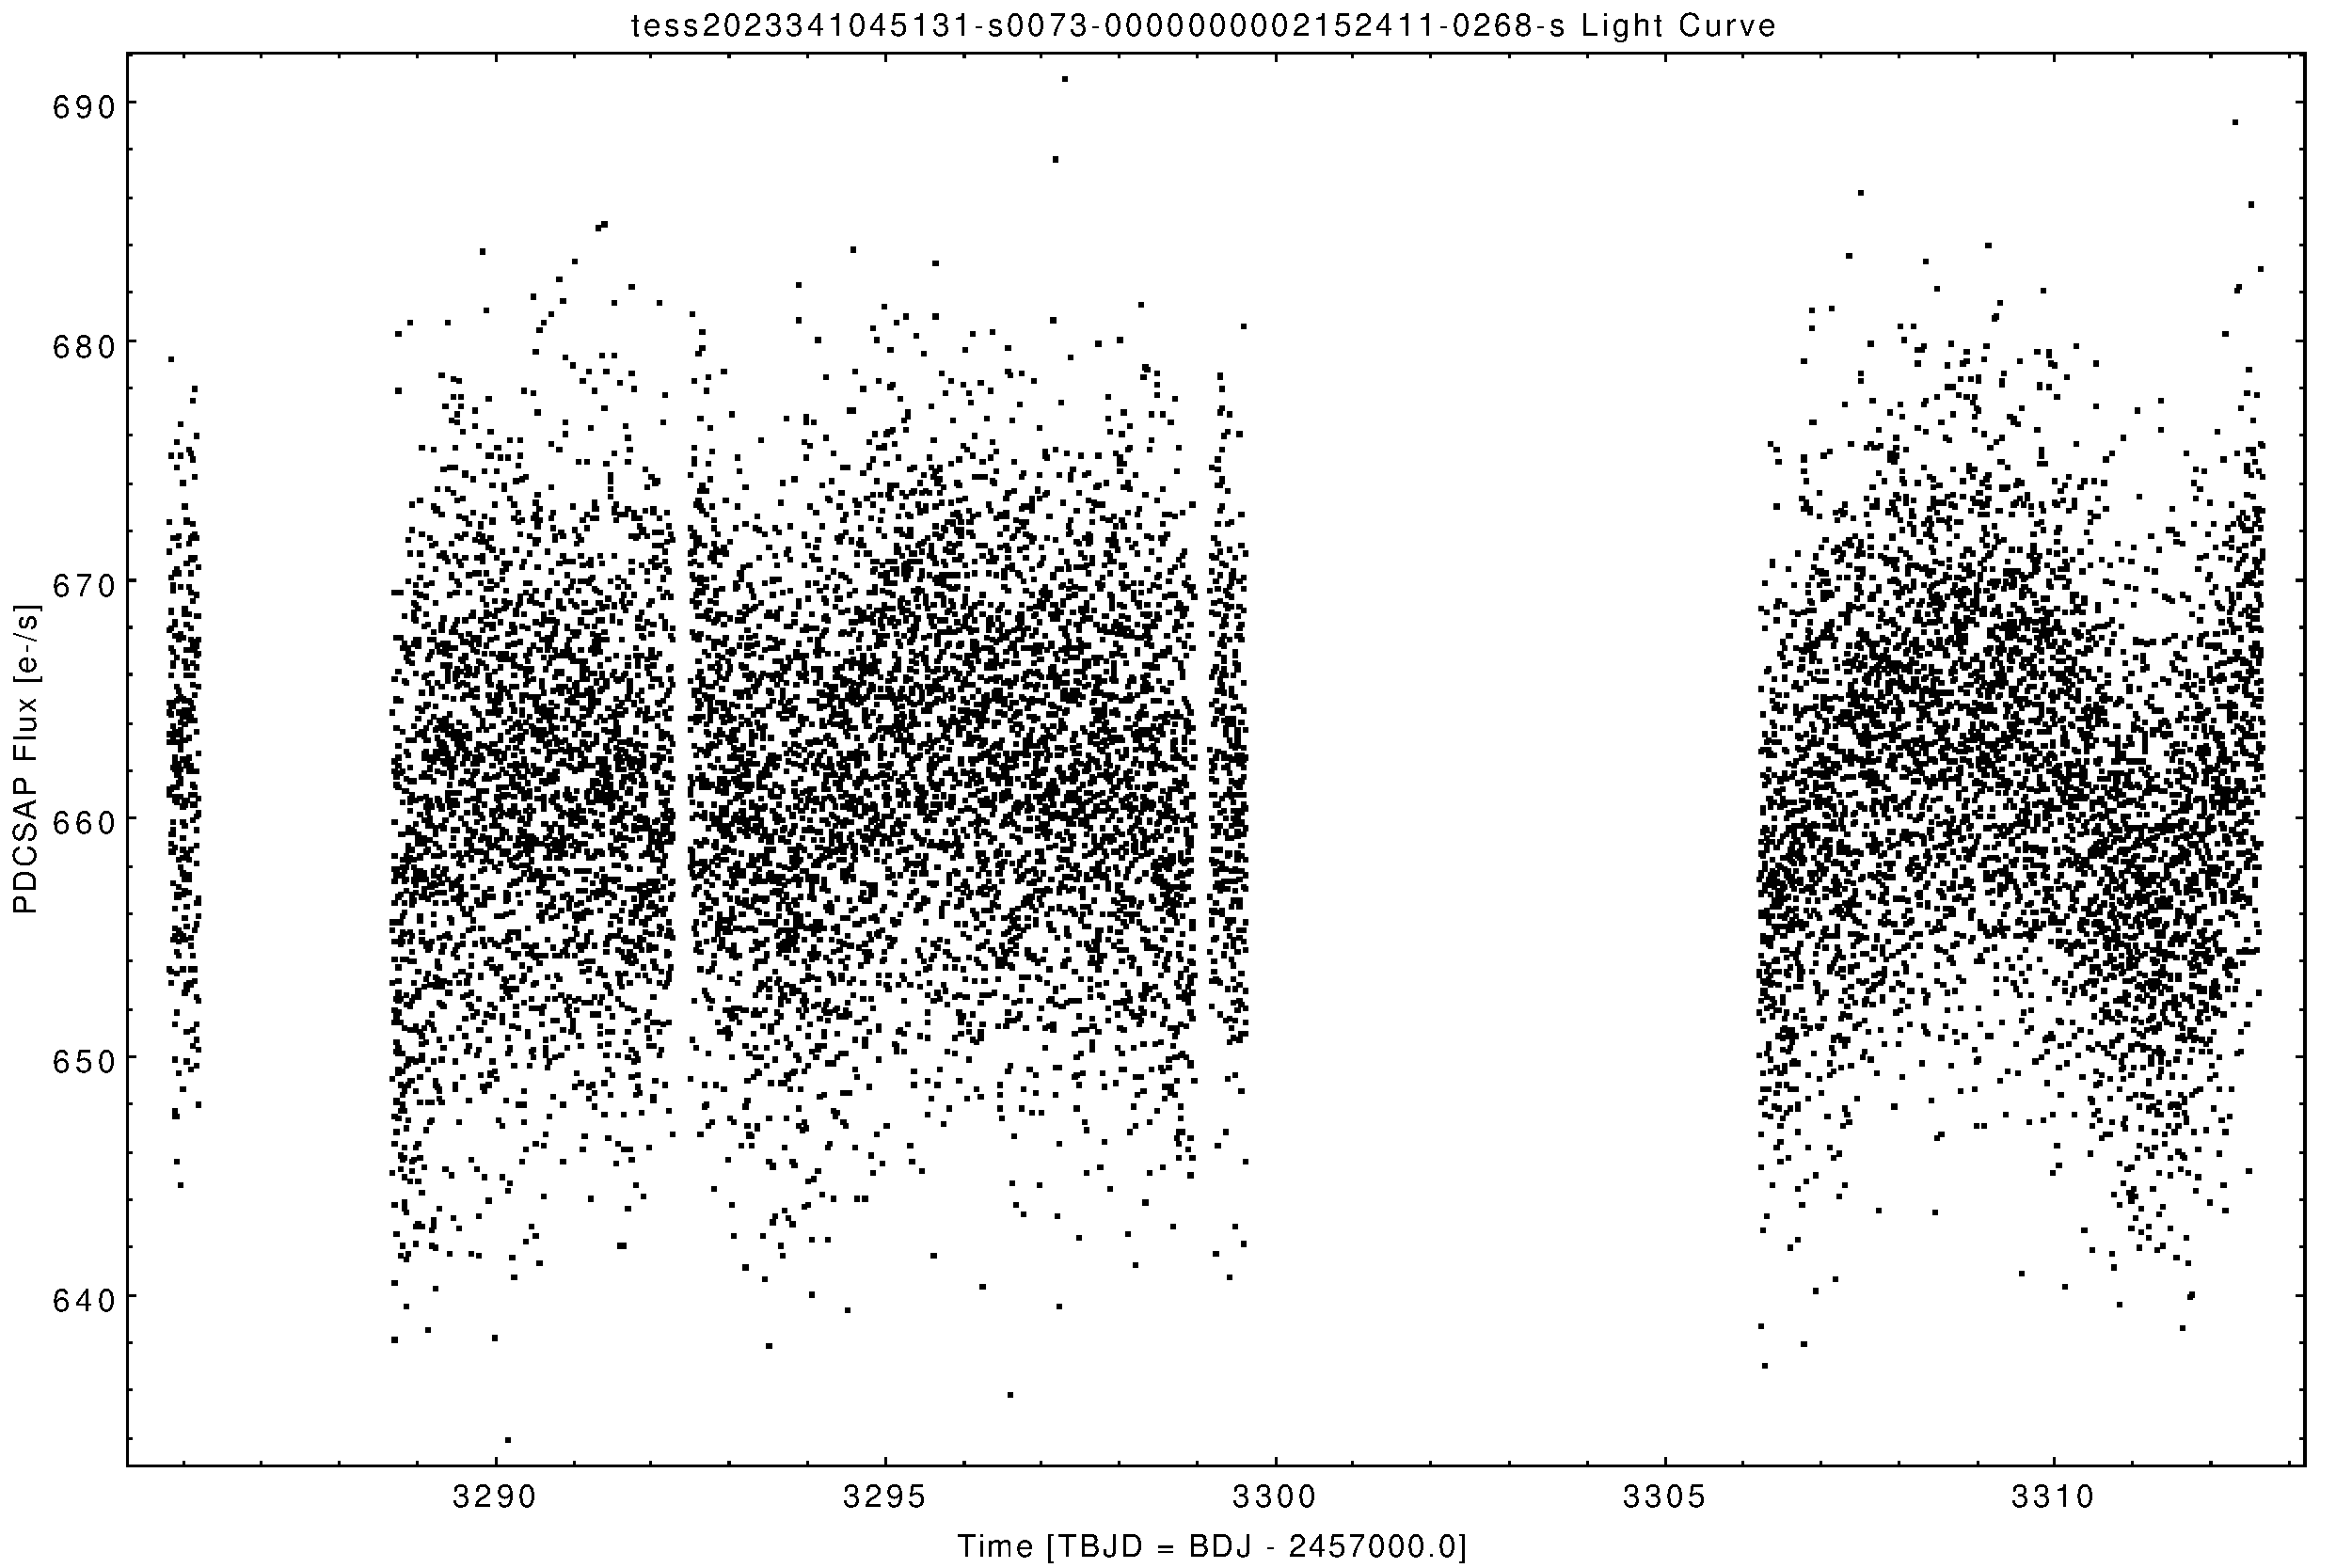
\includegraphics[width = 1\textwidth]{
      lightcurves/tess2023341045131-s0073-0000000002152411-0268-s.pdf}
    \caption{tess2023341045131-s0073-0000000002152411-0268-s light curve}
\end{figure}
\begin{figure}[htbp]
    \centering
    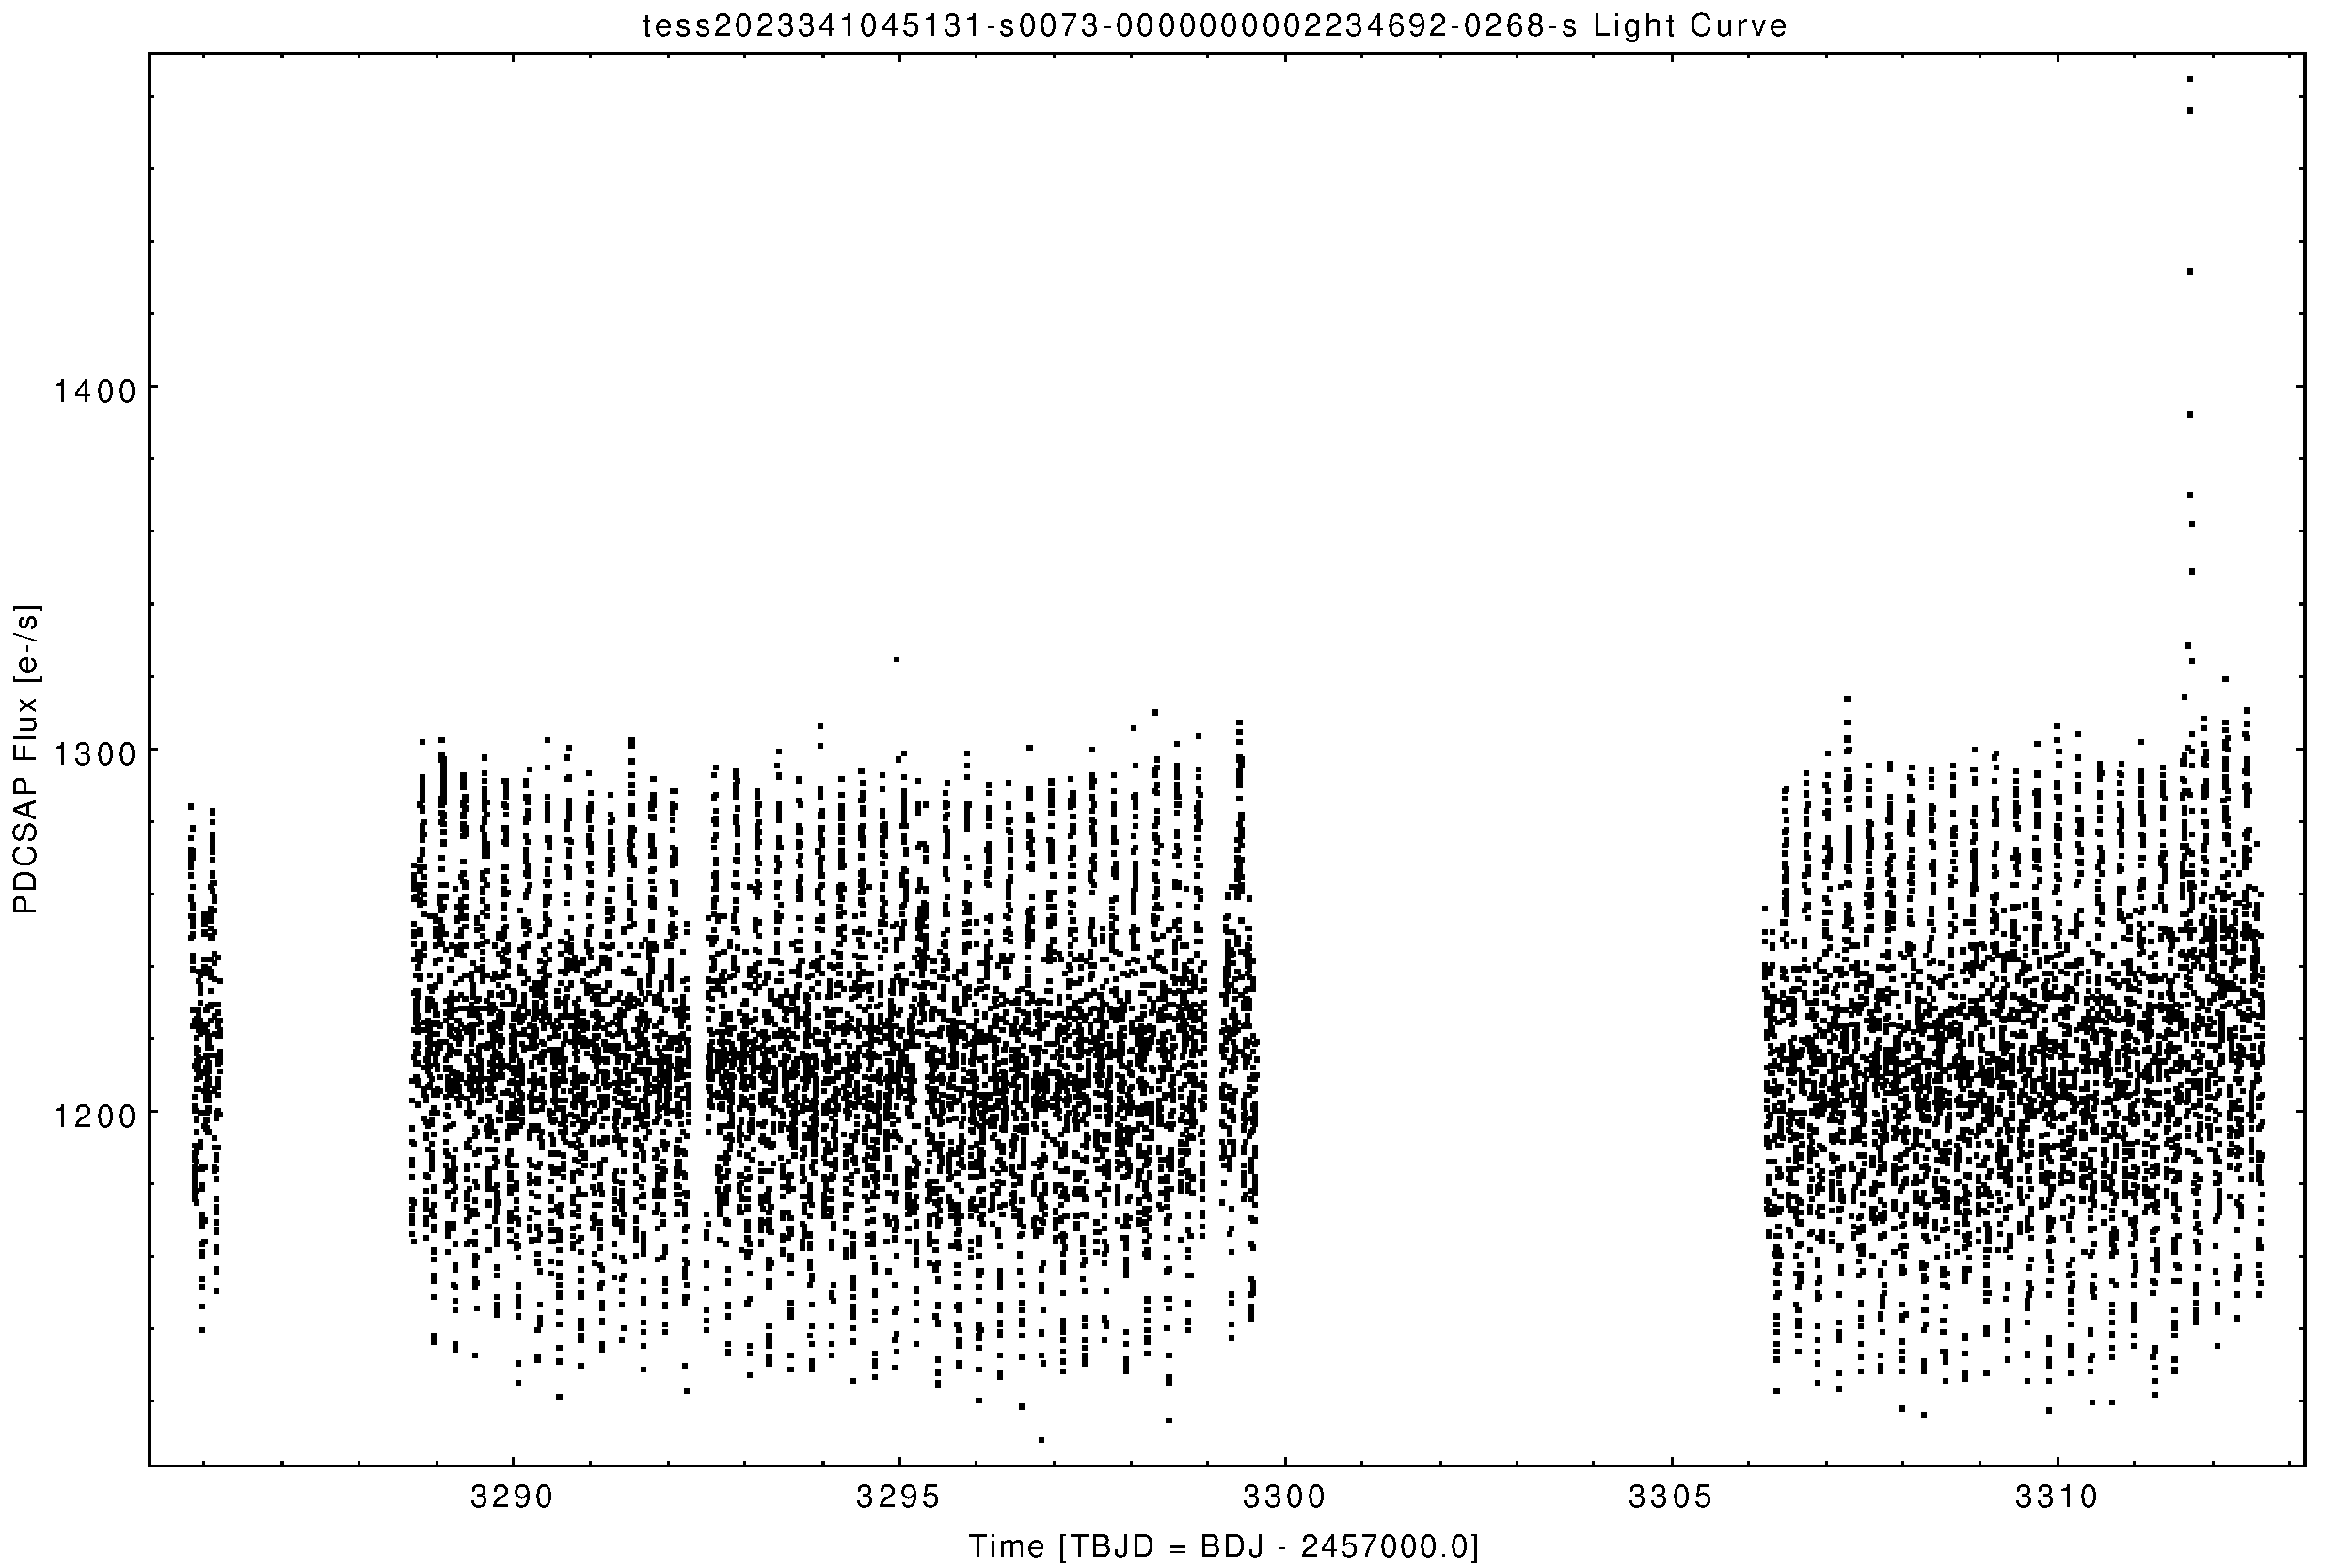
\includegraphics[width = 1\textwidth]{
      lightcurves/tess2023341045131-s0073-0000000002234692-0268-s.pdf}
    \caption{tess2023341045131-s0073-0000000002234692-0268-s light curve}
\end{figure}
\end{document}
